%% Use the standard UP-methodology class
%% with French language.
%%
%% You may specify the option 'twoside' or 'oneside' for
%% the document.
%%
%% See the documentation tex-upmethodology on
%% http://www.arakhne.org/tex-upmethodology/
%% for details about the macros that are provided by the class and
%% to obtain the list of the packages that are already included. 
 
\documentclass[french]{spimubphdthesis}

%%--------------------
%% The TeX code is entering with UTF8
%% character encoding (Linux and MacOS standards)
\usepackage[utf8]{inputenc}
 
%%-------------------
%% You want to use the NatBib extension
\usepackage[]{natbib}

%%--------------------
%% Include the 'multibib' package to enable to
%% have different types of bibliographies in the
%% document (see at the end of this template for
%% an example with a personnal bibliography and
%% a general bibliography)
%%
%% Each bibliography defined with 'multibib'
%% adds a chapter with the corresponding
%% publications (in addition to the chapter for
%% the standard/general bibliography).
%% CAUTION:
%% There is no standard way to do include this type of
%% personnal bibliography.
%% We propose to use 'multibib' package to help you,
%% for example.
%\usepackage{multibib}
 
%% Define a "type" of bibliography, here the PERSONAL one,
%% that is supported by 'multibib'.
%\newcites{PERSO}{Liste de mes publications}
 
%% To cite one of your PERSONAL papers with the style
%% of the PERSONAL bibliography: \citePERSO{key}
%% To force to show one of your PERSONAL papers into
%% the PERSONAL bibliography, even if not cited in the
%% text: \nocitePERSO{key}
 
%% REMARK: When you are using 'multibib', you
%% must compile the PERSONAL bibliography by hand.
%% For example, the sequence of commands to run
%% when you had defined the bibliography PERSO is:
%%   $ pdflatex my_document.tex
%%   $ bibtex my_document.aux
%%   $ bibtex PERSO.aux
%%   $ pdflatex my_document.tex
%%   $ pdflatex my_document.tex
%%   $ pdflatex my_document.tex
 
%%--------------------
%% Add here any other packages that are needed for your document.
%\usepackage{eurosim}
%\usepackage{amsmath}
 \usepackage[]{natbib}

\usepackage{minitoc}

\usepackage{hyperref}

\usepackage{booktabs}
\usepackage{lscape}
%tableau 
\usepackage{multirow}
% subfloat figure
%\usepackage[]{subfig}
\usepackage{subcaption}
\usepackage{tikz}
% eps file
\usepackage{epsfig}
\usepackage[outdir=./]{epstopdf}

\makeatletter
\renewcommand\paragraph{\@startsection{paragraph}{4}{0pt}%
                                      {-3.25ex plus -1ex minus -.2ex}%
                                      {1.5ex plus .2ex}%
                                      {\normalfont\normalsize}}
\renewcommand*\l@paragraph{\@dottedtocline{4}{11.1em}{5em}}
\makeatother
\setcounter{secnumdepth}{4}
\setcounter{tocdepth}{4}
\setcounter{minitocdepth}{4}

\let\subsubsubsection\paragraph
\renewcommand{\theparagraph}{\thesubsubsection.\alph{paragraph}}

\dominitoc

%%--------------------
%% Set the title, subtitle, defense date, and
%% the registration number of the PhD thesis.
%% The optional parameter is the subtitle of the PhD thesis.
%% The first mandatory parameter is the title of the PhD thesis.
%% The second mandatory parameter is the date of the PhD defense.
%% The third mandatory parameter is the reference number given by
%% the University Library after the PhD defense.
\declarethesis[is the one]{This is the one}{17 septembre 2017}{42}
 
%%--------------------
%% Set the author of the PhD thesis
\addauthor[david.strubel.pro@gmail.com]{David}{Strub}
 
%%--------------------
%% Add a member of the jury
%% \addjury{Firstname}{Lastname}{Role in the jury}{Position}
\addjury{Incroyable}{Hulk}{Rapporteur}{Professeur à  la Desert State University }
\addjury{Super}{Man}{Examinateur}{Professeur à l'Université de Smallville}
\addjury{Bat}{Fofi}{Directeur de thèse}{Professeur à l'Université de Gotham City}
 
%%--------------------
%% Change style of the table of the jury
%% \Set{jurystyle}{put macros for the style}
%\Set{jurystyle}{\small}
 
%%--------------------
%% Set the English abstract
\thesisabstract[english]{This is the abstract in English abstract  of the thesis. }
 
%%--------------------
%% Set the English keywords. They only appear if
%% there is an English abstract
\thesiskeywords[english]{Keyword 1, Keyword 2}
 
%%--------------------
%% Set the French abstract
%%\thesisabstract[french]{Ceci est le résumé en français}
 
%%--------------------
%% Set the French keywords. They only appear if
%% there is an French abstract
\thesiskeywords[french]{Mot-cl\'e 1, Mot-cl\'e 2}
 
%%--------------------
%% Change the layout and the style of the text of the "primary" abstract.
%% If your document is written in French, the primary abstract is in French,
%% otherwise it is in English.
%\Set{primaryabstractstyle}{\tiny}
 
%%--------------------
%% Change the layout and the style of the text of the "secondary" abstract.
%% If your document is written in French, the secondary abstract is in English,
%% otherwise it is in French.
%\Set{secondaryabstractstyle}{\tiny}
 
%%--------------------
%% Change the layout and the style of the text of the "primary" keywords.
%% If your document is written in French, the primary keywords are in French,
%% otherwise they are in English.
%\Set{primarykeywordstyle}{\tiny}
 
%%--------------------
%% Change the layout and the style of the text of the "secondary" keywords.
%% If your document is written in French, the secondary keywords are in English,
%% otherwise they are in French.
%\Set{secondarykeywordstyle}{\tiny}
 
%%--------------------
%% Change the speciality of the PhD thesis
%\Set{speciality}{Informatique}
 
%%--------------------
%% Change the institution
%\Set{universityname}{Universit\'e de Bourgogne}
 

%%--------------------
%% Clear the list of the laboratories
\resetlaboratories

%%--------------------
%% Add the laboratory where the thesis was made
%\addlaboratory{Laboratoire Waynes Industry}

\addlaboratory{Laboratoire \'Electronique, Informatique et Image}

%%--------------------
%% Clear the list of the partner/sponsor logos
\resetpartners

%%--------------------
%% Add the logos of the partners or the sponsors on the front page
%\addpartner[image options]{image name}

\addpartner{pdf/le2ilogo}
\addpartner{pdf/cnrslogo}
\addpartner{img/utp-logo}
%%--------------------
%% Change the header and the foot of the pages.
%% You must include the package "fancyhdr" to
%% have access to these macros.
%% Left header
%\lhead{}
%% Center header
%\chead{}
%% Right header
%\rhead{}
%% Left footer
%\lfoot{}
%% Center footer
%\cfoot{}
%% Right footer
%\rfoot{}
 
%%--------------------
% Declare several theorems
\declareupmtheorem{mytheorem}{My Theorem}{List of my Theorems}

%%--------------------
%% Change the message on the backcover.
%\Set{backcovermessage}{%
%	Some text
%}
\newcommand{\tabsimuposeVrep}{% camera pose satelitte
\begin{tabular}{l|ll}
\textbf {Parameters }             		 &\textbf{Value }                                &  \\ \cline{1-2}
\cellcolor[HTML]{F2F2FF}{$z$}        	 & \cellcolor[HTML]{F2F2FF}{[}0.5;1;1.5{]}       &  \\
\cellcolor[HTML]{FFFFFF}$\gamma$         & \cellcolor[HTML]{FFFFFF}portrait or landscape &  \\
\cellcolor[HTML]{F2F2FF}Size of the area & \cellcolor[HTML]{F2F2FF}150x140 px       	 &  \\
\cellcolor[HTML]{FFFFFF}Maximum size of camera projection & \cellcolor[HTML]{FFFFFF}30x22 px & \\
\cellcolor[HTML]{F2F2FF}Number of waypoints & \cellcolor[HTML]{F2F2FF}22        		 &  
\end{tabular}
}
\newcommand{\tabsimuposeIUTcube}{% camera pose satelitte
\begin{tabular}{l|ll}
\textbf {Parameters }             			&\textbf{Value }                              	 &  \\ \cline{1-2}
\cellcolor[HTML]{F2F2FF}{$z$}        		& \cellcolor[HTML]{F2F2FF}{[}0.5;1;1.5;1.75{]}   &  \\
\cellcolor[HTML]{FFFFFF}$\gamma$        	& \cellcolor[HTML]{FFFFFF}portrait or landscape  &  \\
\cellcolor[HTML]{F2F2FF}Size of the area 	& \cellcolor[HTML]{F2F2FF}380x310 px       		 &  \\
\cellcolor[HTML]{FFFFFF}Maximum size of camera projection & \cellcolor[HTML]{FFFFFF}42x54 px & \\
\cellcolor[HTML]{F2F2FF}Number of waypoints & \cellcolor[HTML]{F2F2FF}75       				 &  
\end{tabular}
}

\newcommand{\tabsimuposeTorcy}{% camera pose satelitte
\begin{tabular}{l|ll}
\textbf {Parameters }             			&\textbf{Value }                              	&  \\ \cline{1-2}
\cellcolor[HTML]{F2F2FF}{$z$}        		& \cellcolor[HTML]{F2F2FF}{[}1;1.5;1.75{]}      &  \\
\cellcolor[HTML]{FFFFFF}$\gamma$        	& \cellcolor[HTML]{FFFFFF}only portrait 		&  \\
\cellcolor[HTML]{F2F2FF}Size of the area 	& \cellcolor[HTML]{F2F2FF} 278x214 px        	&  \\
\cellcolor[HTML]{FFFFFF}Maximum size of camera projection & \cellcolor[HTML]{FFFFFF}35x52 px & \\
\cellcolor[HTML]{F2F2FF}Number of waypoints & \cellcolor[HTML]{F2F2FF}25       				&  
\end{tabular}
}



\newcommand{\tabsimuposeCalvisson}{% camera pose satelitte
\begin{tabular}{l|ll}
\textbf {Parameters }             			&\textbf{Value }                              	 &  \\ \cline{1-2}
\cellcolor[HTML]{F2F2FF}{$z$}       	 	& \cellcolor[HTML]{F2F2FF}{[}1;1.5;1.75{]}       &  \\
\cellcolor[HTML]{FFFFFF}$\gamma$        	& \cellcolor[HTML]{FFFFFF}portrait or landscape  &  \\
\cellcolor[HTML]{F2F2FF}Size of the area 	& \cellcolor[HTML]{F2F2FF}1113x848 px       	 &  \\
\cellcolor[HTML]{FFFFFF}Maximum size of camera projection & \cellcolor[HTML]{FFFFFF}69x104 px & \\
\cellcolor[HTML]{F2F2FF}Number of waypoints & \cellcolor[HTML]{F2F2FF}110       			  &  
\end{tabular}
}

\newcommand{\tabsimuposeFley}{% camera pose satelitte
\begin{tabular}{l|ll}
\textbf {Parameters }            		 &\textbf{Value }                           	  	&  \\ \cline{1-2}
\cellcolor[HTML]{F2F2FF}{$z$}       	 & \cellcolor[HTML]{F2F2FF}{[}0.6;0,8;1{]}        	&  \\
\cellcolor[HTML]{FFFFFF}$\gamma$       	 & \cellcolor[HTML]{FFFFFF}portrait or landscape 	&  \\
\cellcolor[HTML]{F2F2FF}Size of the area & \cellcolor[HTML]{F2F2FF}895x502 px          		&  \\
\cellcolor[HTML]{FFFFFF}Maximum size of camera projection & \cellcolor[HTML]{FFFFFF}75x50 px & \\
\cellcolor[HTML]{F2F2FF}Number of waypoints & \cellcolor[HTML]{F2F2FF}80       			  &  
\end{tabular}
}

\begin{document}
 
%%--------------------
%% The following line does nothing until
%% the class option 'nofrontmatter' is given.
%\frontmatter

%%--------------------
%% The following line permits to add a chapter for "acknowledgements"
%% at the beginning of the document. This chapter has not a chapter
%% number (using the "star-ed" version of \chapter) to prevent it to
%% be in the table of contents
\chapter*{Remerciements}
 ma famille  et plume toufia 
%%--------------------
%% Include a general table of contents
\tableofcontents

%%--------------------
%% The content of the PhD thesis
\mainmatter
 
\part{Contexte et Problématiques}

\chapter{content/introduction/}
  
\section{Context and motivation}

Ce squelette d'écrit quelques éléments pouvant vous aider pour écrire votre ouvrage de thèse.
Un plan typique d'une thèse scientifique est également proposé. ss\cite{Wang1996} 122* 
teste cite \cite{118*}


\section{scope and challenges}
quelle son les point  bloquant  en qlq ligne 
\section{Contribution }
postionement de  camera :  problem formulation  
						   GA 
						   results 
CPPP :  decoupe du problem
		par plan
		result and solution 
\section{Organisation }

\begin{emphbox}
	do some things!
\end{emphbox}


%\chapter{chap1test}

%\chapter{\'Etat de l'art}z

\chapter{State Of Art}\label{chap:stateOfTheArt}

\minitoc

The surveillance and control domain is a wide field of research which contains a lot of aspects such as: object tracking, object recognition, 3D mapping and area coverage among others. Our work focused specifically on the latter, i.e. finding a procedure which allows to capture a minimal number of images of a given area maximizing the coverage of the area.    
This can be achieved using a set of visual sensors. Many parameters have thus to be taken into account: size and shape of the area itself, field of view of the cameras, number of cameras (or views) to name a few. The following chapter will survey the different methods and techniques proposed in the literature to solve this problem. Keeping in mind that our  final goal is to find out a technique that works both indoor and outdoor, flexible enough to handle two scenarios: (1) a set of cameras observing simultaneously the area; (2) a single camera moving along a pre-computed path to cover the area. 

\section{Camera positioning }\label{sec:camerasPositioning}

The first step for solving the area coverage problem is the camera positioning, i.e. how to estimate an optimal viewpoint selection to ensure an acceptable coverage. It is known that an efficient camera positioning is a bottleneck in many applications, as for example in the video surveillance field \cite{11*herrera2012,12*soto2009,18*ding2012,151*zhao2013,84*xu2011}, where an efficient camera positioning is essential to monitor correctly an area.  
The following section will deal with the question of: 
\begin{itemize}
\item[-]What is a good position and orientation for a camera (i.e. a good camera pose)?
\item[-]What are the purposes of the application requiring camera positioning?

\end{itemize}
These questions have already been investigated and some solutions have been proposed in the literature. 


%\subsection{Efficient pose in a camera network: challenges and objectives}
%The first point to address is defining the pose of the camera (or set of cameras). In computer vision, the pose of a camera is composed of its position in space and orientation (or viewing direction), i.e. of 3 translations and 3 rotations in a world coordinate frame. The second point to be addressed is how to define a "good" or "optimal" camera pose(s)?\\
% To do so, it is essential to identify the purposes, tasks and priorities of the application: 
% \begin{itemize}
% \item [-] What is the final goal?
% \item [-] What are the important features for the application (e.g. to track an object, to have a high-resolution mapping, etc.)?
% \item [-] What are the shooting conditions and physical constraints?
% \end{itemize}
%   All of these aspects will have an incidence on the definition and formalization of a "good camera poses". For instance, in \cite{22*zhao2008}, the purpose is to detect tags placed on people torso which forces the camera to be positioned at a certain height with a viewing direction almost parallel to the ground; on the contrary, in \cite{146*li2011}, a camera is mounted on a UAV to monitor a vast outdoor area, which forces it to have a viewing direction almost perpendicular to the ground. 
%
%%It is important to do not confuse the finality and the objectives. For example video surveillance is the finality but the coverage of an area or the target tracking, it is required to have an efficient surveillance. The coverage is one of the objectives the most interesting and the most common about cameras positioning.
%% !!!!!!!!!
%%  The objectives are different from the finality. The objectives are the most important elements to take in consideration in order to place the set of cameras. When the finality is the global application, as for example video surveillance is the finality but the coverage of an area, the target tracking is required to have an efficient surveillance. The coverage is one of the objectives the most interesting and the most common about cameras positioning.
%%!!!!!!!!!
%%The coverage can be applied on cover each side of an object (as  in [142*]). But in most of the case the coverage is applied on area ( inside or outside). 
%
%%To have a clever and efficient cameras positioning system different aspects must be studied. First, to pose efficiently a set of cameras it is useful to know what does it mean efficient for the camera pose. To do that the objective of the cameras network have to be defined clearly. 
%
%%The objectives  vary and depending than the finality the cameras position is greatly affected.
%These two articles share the same objective, i.e. to get the best possible coverage of an area, but since the constraints and secondary objectives they must comply with are different (e.g. number of cameras, resolution, luminosity, tracking, etc.), it leads to different formulation and approach. 
%
%The next section focuses on positioning the camera to maximize viewing areas. The viewing area or coverage rate of the area is directly related to the estimated position of each camera and their orientation. To get the best coverage, it is essential to find the best pose for each camera, depending on the constraints and possible secondary goals.\\
%%(!!!! The finality and thus the secondary objective greatly, have an important influence on the camera positioning.!!!!!)
%
%Camera positioning for maximizing the coverage rate has been studied these past decades, using many different approaches. The following sub-section will provide an overview of different ways of defining the coverage drawn from the literature.
%
%%The approaches was greatly influenced by finality. In fact the finality will involve a main objective and potential some other secondary objective with their constraint. In many case the coverage maximization is the main objective but the impact of the secondary objectives are not negligible. In numerous cases, the maximization of the coverage is only the first part of the problem, hence the importance of secondary objectives.
%%The following sections are dedicated on what kind of area is covered  what is exactly the coverage with the secondary objectives  associated too.
%%%Indeed to maximize the coverage rate by optimizing the cameras position has been studied this past decade, using many different approaches. \\
%%%His approach is applicable depending on the formulation of the constraints and objectives. In numerous cases, the maximization of the coverage is only the first part of the problem, hence the importance of secondary objectives.\\
%%%The following part is focused on what kind of area is covered what is exactly called coverage and with the secondary objectives associated too.
%
%\subsection{Objective: Coverage }\label{sec:FirstObjCover}
%
%Before formalising the coverage rate to be maximised, it is necessary to define exactly what is meant by coverage: is the aim to maximise the surface area of a three-dimensional object or a 2D zone whose perimeter has been circumscribed? Is there a priori knowledge of the area to be covered (its perimeter, its bounding box, etc.) or not? Is the area to be covered homogeneous or does it contain prioritized sub-areas? 
%% Among the huge possible definition more or less restrictive the more interesting to studied is discussed: 


\begin{itemize}
%-------------------------------------------------
\item Object coverage: \\
\begin{figure}[t!]
\center
\minipage{0.75\textwidth}
   \includegraphics[width=\linewidth]{img/objectCoverFrom142.png}
  \caption{Full coverage of an object in the 3D space. The coverage is made by selecting a set of adapted waypoints. The coverage must be good enough to enable reconstruction of the 3D shape of the object without any occlusion. Result here are obtained by the method of Hoppe et al. \cite{142*hoppe2012}.}\label{fig:ObjectCover142}
  \endminipage\hfill
\end{figure}
   %The definition of a coverage can be varied this is a good example. 
   In Hoppe et al. \cite{142*hoppe2012} a good coverage is defined by the ability to have full 3D reconstruction of an object (in their 3 dimensions) with no occlusion. In this work, some prior knowledge on the object is exploited such as a rough surface description (mesh). The camera follows a trajectory "around" the object and its viewing direction is oriented towards the center of the mesh (see Figure \ref{fig:ObjectCover142}). 
  Since it is a matter of covering the 3D surface of an object, in a next-best-view strategy, this application remains too far from the one we wish to implement.  It is therefore barely applicable to our problem. \\ 
   %-------------------------------------------------
   \item Path to cover: \\
   \begin{figure}[t!]
\center
\minipage{0.75\textwidth}
   \includegraphics[width=\linewidth]{img/PathToCover[81].png}
  \caption{Illustration of "path to cover" of Nikolaidis et al. \cite{81*nikolaidis2009}. The aim is to focus on covering a road (walking path) in a small room by using only 3 cameras. }\label{fig:pathToCover81}
  \endminipage\hfill
\end{figure}
   The point here is to observe the entire trajectory commonly taken by users (car, pedestrians, …). When the area to cover is a known place, the main trajectory taken by the users can be estimated or extracted \cite{27*bodor2005}. If the area to cover is a road, for instance, then the trajectory of the driver is known \cite{14*lu2011}. In this condition, the aim is to cover the common trajectory of the user as presented in  \cite{14*lu2011,27*bodor2005,30*bodor2005,81*nikolaidis2009} (see the Figure \ref{fig:pathToCover81}). The path coverage is interesting due to the restricted area to cover: not an entire area, but only a path within a given area, that can be seen as a priority sub-area. \\
   %-------------------------------------------------
   \item Coverage priority: \\
      \begin{figure}[t!]
\center
\minipage{0.75\textwidth}
   \includegraphics[width=\linewidth]{img/MapRoI165.png}
  \caption{Map of an area to cover with crucial sub-area (region of interest), the normal sub-area  and obstacle. This map is an example of area coverage  introduced in  Jiang et al. \cite{165*jiang2010}. }\label{fig:MapRoI165}
  \endminipage\hfill
\end{figure}
   A natural way of defining the coverage in a context of insufficient number of cameras, is to define as priorities.
    In \cite{84*xu2011,165*jiang2010,171*horster2006}, some pre-defined regions are set as "priority" and called respectively "region of interest", "crucial sub-area" (see Figure \ref{fig:MapRoI165}) and "importance space weighting".  In the proposed solutions  by \cite{84*xu2011,165*jiang2010,171*horster2006}, the camera poses are in priority affected to this specific and restricted region which has the effect to neglect the other parts of the area. \\
If the environment is composed of some regions of interest, there should be also "normal" sub-areas. These "normal sub-areas" should be covered, but with lower priority. Furthermore, some  sub-areas can be defined as "no interest", which mean "not to be covered". In \cite{165*jiang2010,171*horster2006} for example, the obstacles are defined as "no interest" regions with also the consequence to  be occluding area. The idea is to keep a maximum of freedom in the camera network positioning and allow the system to handle local priority and constraints.\\
%-------------------------------------------------
\item Inside or outside area:\\ 
Another important feature to define the coverage is related to indoor/outdoor scenes. The area to cover can be typically a room with walls (indoor). Each wall must be a considered as an obstacle occluding the camera field of view,  which results in having to manage the visibility of the environment according to these obstacles and to the position of the cameras. For outdoor scenes, it is often necessary to take into account the size of the environment according to the reduced field of view of the camera. This has the effect of increasing the number of required cameras (or views) and leveraging the combinatory. 

%(also in the inside area the constraint must be the restricted posibel position of the camera (the camera must be placed on the wall for exemple))
   
\end{itemize}
  
\subsection{Additional constraints} \label{subsec:AddConst}
The common points in all the examples discussed is the aim of maximizing the coverage rate. The positioning of the cameras, and its effects on the coverage rate, is thus constrained by the application itself, the context  and the type of observed scenes.\\
%!!!!!!
%The common points in all this coverage definition is the importance to maximize it, despite the other objectives. In the examples presented the coverage was always the first and for some of them the only objective. Despite the interest for maximizing the coverage some other elements has to be taken in account to have a useful cameras position depending on the finality. 
Of course, additional constraints can have also a significant impact on the camera pose. Some of the more common constraints found in the literature are listed below:\\
\begin{itemize}
\item  The numbers of cameras: \\ In many cases,  the number of cameras used for the coverage should be minimised such as in  \cite{151*zhao2013,171*horster2006,22*zhao2008}. Limiting the number of cameras is primordial to decrease the computation time and the bandwidth. It also reduces the cost of the setup \cite{82*chrysostomou2012}. Reducing the number of cameras and optimizing their poses to get an optimal coverage are closely related tasks, not necessarily competing. Too few cameras can shrink the coverage rate by leaving black-holes in some areas of the scene. Too many cameras can result in too much overlaps and unnecessary redundancies.\\

\item Object tracking: \\
\begin{mfigures}[!]{Illustration of an covered area for tracking target. Experiment  from Ding et al. \citep{18*ding2012} }{fig:Tracking18} \centering
\mfigure{width=.65\linewidth}{img/coverageTrackingDing[18]a.png}{Initial coverage for 5 cameras dedicated to detect the  input of target.}{subfig:taget18a}
\hspace{1cm} \\
\mfigure{width=.65\linewidth}{img/coverageTrackingDing[18]b.png}{The covered area when the objective have to track several targets.}{subfig:taget18b}
\end{mfigures}	
 Constraints can arise by the objective of detecting and localising a given target \cite{18*ding2012,12*soto2009,23*liu2009,39*wu2011,40*sohrabi2000,22*zhao2008}. In such a case, camera poses must be estimated in order to track one or more targets, and possibly, be dynamically adapted. These applications very often requires an adaptation of the camera orientation (viewing direction) more than its position. This is the reason why previous work used PTZ cameras (Pan, Tilt and Zoom) as in \cite{18*ding2012,38*liu2010,12*soto2009} (see Figure \citep{18*ding2012}).
Keeping a full area covered and at the same time tracking efficiently one or more targets can be contradictory. The solution is then the result of a trade-off between coverage and tracking, as in \cite{18*ding2012} and \cite{38*liu2010}.
 In Liu et al. \cite{38*liu2010}, target tracking in a wide area is decomposed in two steps: detection and localization. Each of these steps is performed independently on each camera. Area coverage is essential to detect the targets, less for localization as the priority is, in this step, to track a target previously detected within the covered area. In the entire camera network used, one camera may be in detection mode while another is in location mode. Obviously, by adding target tracking as a constraint, camera poses and coverage are usually less efficient because of the sub set of cameras  assigned to the tracking.  \\

\item  Luminosity and environmental setup:\\ Intrinsic image quality is also a constraint that can guide area coverage. The quality of an image can result in sufficient brightness or an almost uniformly distributed histogram. In other words, the captured images must be such that they guarantee a usable signal. For example, Reddy et al. \cite{33*reddy2012} addressed first the coverage problem of a complex area and in second time,  target localization. In order to decide which target must be tracked, the quality of the image is taken into account to avoid dark areas where the target is hardly detectable. In this case, the tracking and coverage trade-off discussed in the previous paragraph is  ruled by the image quality. \\

\item  Energetic cost:
\\ Authors suggests to estimate camera positioning or path planning by minimizing a cost function that represents the energy consumption, such as in  \cite{38*liu2010,42*bulusu2001}. For instance, in Lui et al. \cite{38*liu2010}, the  objective is to cover most of an area to detect whether a target is entered in the scene or not. Secondly, the target is tracked by smart and autonomous cameras of the network. The camera set  is randomly distributed in the area and the coverage problem represents, in this case, the selection of the best cameras in order to detect the target. The selection of the cameras is estimated by both maximizing the area coverage and minimizing the energy consumption. The consumption can be consequently reduced by restricting the number of cameras set in detection mode. Indeed, the cameras are more or less power-consuming depending on the activated mode (which can be "detection", "tracking" or "sleep"). If we consider now path planning, the energy cost can be represented by the distance between two cameras or views and energy minimization is equivalent to finding the shortest path \cite{191*di2016,218*meiting2007}.  
\\
\item Multi coverage:\\
 Among the numerous possible constraints, the multi-coverage is interesting (as for example in \cite{149*mavrinac2013,151*zhao2013,152*wang2009,174*zhang2016,175*medhi2013}). It can be seen as a coverage problem where one or a few specific sub-areas must be covered by a minimum of $k$ cameras at the  same time, that is why it is also called $k$-coverage. Multi-coverage does not necessarily mean priority: a sub-area which have to be covered by several cameras is not necessarily a sub-area which must be covered in priority (more details in Section \ref{sec:zoneOfInterest}). However, mobilizing multiple cameras in a given sub-area means that fewer cameras can be used to cover the rest of the overall area. This effect can be compensated by adding cameras, if allowed. Contrarily, full-coverage of the area and k-coverage of some sub-areas will conflict and lead to a trade-off. 
 %This secondary objective in the case of limit will generate a conflict between the full coverage of the area and the $k$-coverage requirement even more with a restricted number of cameras. 
\\ 
\item  Resolution:\\ In order to keep or increase the quality of the captured images, a minimum resolution threshold or value can be fixed and used as a constraint \cite{27*bodor2005,33*reddy2012,171*horster2006,152*wang2009,43*erdem2006}. The focal length, the size of the pixel grid or the camera-target distance can serve as a measure for the resolution. However, in many applications, it is easier to adapt the distance than changing the focal length (which can be fixed and affect the calibration) or, of course, changing the size of the pixel grid. In most of the previously cited works, the distance from the target to the camera along the optical axis is therefore used as a measure for the resolution.\\
%The resolution is also model as the acceptable the depth of field.
Full coverage will tend to move the cameras at the farther distance (or higher elevation) in order to maximize the field of view. Resolution constraint will impose the cameras to be positioned at a certain range of distance or elevation. Full coverage and resolution constraint will lead to a trade-off between guaranteeing most of the area to be covered and a sufficient image resolution. The trade-off is particularly beneficial when the number of cameras is more important than the optimal need, in this case, the distance will be reduced and the resolution subsequently increased. \\
   In \cite{33*reddy2012} the problem has been formalized by using a Gaussian function in order to define the proper distance between the cameras and the target to keep an acceptable resolution for the application. \\
Here, the depth of view is used to define the range of distances. The focus point and the aperture of the camera will define the optimal distance and range in which the target is optimally focused \cite{193*fu2014}. Constraining the positioning with the depth of view can be seen somehow as a constraint on the resolution itself. 

\end{itemize}

The constraints are numerous and varied, we just introduced a few of them which seems interesting to us and related to our work. Among them, some are closely related and can be interconnected, they can even be combined as in \cite{33*reddy2012}, where the targets coverage, luminosity, resolution, are all associated to find the best camera positions maximizing the area coverage and the tracking target with good visibility condition. \\
One interesting point to study is the impact of these constraints on the full coverage itself as we have seen that they introduce a trade-off between their own particular goal and the main goal of area coverage but also between themselves. No need to say thus, that the constraints have to be chosen carefully and accordingly weighted as in any multi-objective problems. 


\subsection{Art gallery problem} \label{sec:AGP}
%Once the objectives defined the next step, is to know how to represent the problems. To do that manly 2 different class  of problems have to be studied. The first is from the geometrical problem called  the Art galery problms.

%The previous section was focus on the objectives definition as well as the finality around the sensors and cameras position

%Until now the problem was presented in term of objectives and constraint in order to be used in a concrete situation.

The Art Gallery Problem (AGP) is a theoretical and historical problem closely related to the camera positioning. The AGP is commonly cited  in the literature as a source of the problem for camera positioning (for full coverage). It is also commonly used to estimate the complexity of the task (notably due to the room shape) and  as starting point to find an appropriate solution. 
The problem of cameras positioning can be formulated as the AGP paradigm (as example \citep{44*chvatal1975,53*packer2008,149*mavrinac2013}). For these reasons, the AGP has to be well understood before going further.

%Until now the problem of coverage was studied to place cameras. The use of cameras (fix or mounted on mobile robot) are the limited field of view  and  depth field of the sensor. An interesting paradigm closely related is to use human guards  instead  of the set of cameras.  This paradigm is called the Art Gallery Problem (AGP). The AGP is an interesting  paradigm with propose some efficient solution. 

In the following sections a definition of the AGP is given with a brief history. After a more general introduction to AGP, we will describe some interesting solutions found in the literature and discuss their limitations.

%The problem of camera positioning is a tricky problem. The positioning of the set of cameras depend on many factor. To solve this problems is importatant to know more about the relat
% %finality of the camera networks and the formulation the camera pose will be affected.\\
%% Once the objectives defined ( see section \ref{sec:camerasPositioning}) the next step, is to know how to represent the problems. To do that manly 2 different paradigms have to be studied.
% The first is from the geometrical problem called the Art Gallery Problem (AGP) formulation is commonly and historically borrowed as is presents in the following section with a fast definition of the problems, the solution used and the limit of this paradigm.


	\subsubsection{Definition of the paradigm} \label{sec:AGPdef}
	\begin{figure}[t!]
\center
\minipage{0.65\textwidth}
   \includegraphics[width=\linewidth]{img/AGP3.png}
  \caption{Illustration of the AGP. The gallery is covered by  4 guards ($x_1;...;x_4$) for a polygon  composed by $n$ vertice ($v_1;...;v_n$).}\label{fig:AGP}
  \endminipage\hfill
\end{figure}
	The art gallery problem is a geometrical problem introduced by Victor Klee in 1973. The problem was the estimation of the number and the position of useful guards to cover an art gallery. 
The particularity of an art gallery is the complexity of the room shape, with many walls to place the paintings. The shape complexity of the room make the estimation of guards number even more difficult.\\
In order to formulate properly the problem, the room is assimilated as a polygon $P$, composed of $n$ vertices ($v_1; v_2;…v_n$). The vertices are linked by $n$ edges ($v_1 v_2;…; v_{n-1} v_n$) to make the shape of the Polygon $P$ (or room).

A guard $x$ is inside the room $x \in P$. A guard $x$ can cover or see any point $y \in P$ if the segment $xy$ is not intersected by one of the boundaries (walls) of the polygon $P$, in order to have $ xy \subseteq P$.
The polygon $P$ is considered as fully covered when for any position of the point $y$ in the polygon, at least one guard can see it .\\
A guard $x$ can have a $360^\circ$ field of view to cover all around him, with no depth of field limitation (except the wall obstacles). Clearly that means the guard can see and monitor the entire room from one side to the other side if there is no obstacles around to occlude its vision. For example, if the shape of the room is a triangle, quadrilateral or another simple polygon, at any position taken by one guard, this guard can monitor all the area despite the size of the art gallery (see Figure \ref{fig:AGP}). 

When the polygon is more complex, it is necessary to estimate the minimum number $g$ of guards $x$ and the position of the guards in polygon $P$. 
 The set of minimum number of guards are listed in $X$. Where $X$ contains the useful $x$ to fully cover the polygons $P$, with $g$ the minimums number of guard in order to have a set of points $X=\{x_1…x_i…. x_g\}$. So that every point $y$ in $P$  are cover by at least on guard $x$ of the set of $X$. \\
The AGP in addition to estimating the numbers of guards,  is also interested in finding the optimal position of this restricted number of guards. 
These two questions can be solved at the same time by using one of the solutions proposed.


	\subsubsection{Solutions }
	
	The advances on the AGP since its formulation in 1973 are numerous. The following paragraphs present some of the main proposals and contributions..\\
	 The first, and one of the most important, is the proof given by Chvàtal in 1975 \cite{44*chvatal1975}.  The proposed polygon must be covered by a minimum of guards, the proof of Chvàtal links the minimum number of guards $g$ to the number of vertices $n$. 
A polygon composed by $n$ vertices need in the worst case a minimum number of guards equal at $n/3$. The Chvàtal proof is based on the triangulation of the polygon. The triangulation is made based on the vertices of the polygon.\\
	 % For a polygon composed by $n$ vertices in the worst case the minimum guard necessary to cover it, is $X=n/3$.
	     The proof given by Chvàtal is also confirmed by the work of Fisk  few years later (1978). The work of Fisk is also based on triangulation and colouring node. It is probably the easiest way to understand and also give a solution to estimate the pose of each guard. It is recommended to begin by the Fisk proof before the Chvàtal one, despite the chronology order as it is recommended in \cite{219*orourke1987}. The book of O'Rourke et al. \cite{219*orourke1987} is an early work about the AGP with the formulation, proofs and advancement of the field clearly explained. \\
After the important work of Chvàtal which enable the estimation of the minimum number of guards in the worst case consequently fix a limit to the AGP. Thus, the research has been oriented toward the optimal guard positioning. The goal is to find the best algorithms to solve the AGP for all kind of polygon while reducing the complexity in time (reducing the $O(...)$).\\
%Once the proof of the minimum number in the worst case founded the objective became to find an optimal guard position for all kind of polygon in reasonable time. \\
In perspective, the work of Toussaint and Avis (in 1981) is the reference and propose a solution working in $O(n log n)$. This work has been followed and upgraded until the solution of Couto, Resend and Souza  2011 \cite{224*couto2011}. The solution  finally proposed reduce the complexity to $O(n^3)$ in the worst case. 

%It is a short overview of the AGP solution but also the solution proposed are very specific to the AGP and cannot be re-use for problem little different.

	
	\subsubsection{Limit of AGP and camera coverage relation}

The AGP can be considered as a reduction of the best camera poses estimation to maximize the coverage of a complex area. Based on the algorithms developed to solve the AGP and the strong relation between AGP and the cameras positioning (for maximum coverage problem), loigically,  some proposed algorithms have been developped. They try to extend the AGP to the  problem of camera positioning as example in \cite{221*fleishman2000,33*reddy2012,43*erdem2006}.\\
%The problem of positioning cameras for maximum coverage is quite close then the AGP. The AGP is a reduction of the camera positioning for a total coverage of a complex areas. The camera positioning is the logical continuation of AGP and once the AGP is solved , the problem can be extended as is for example show in \cite{221*fleishman2000,33*reddy2012,43*erdem2006}.
The algorithms developed for AGP cannot be applied directly on the problem of cameras positioning for maximum coverage. The main reasons are the cameras limitations such as the field of view and the depth of field (see \cite{82*chrysostomou2012,170*yabuta2008}). The cameras limitations makes  unreadable the algorithm proposed to solve the AGP; because the AGP is considering the guard with no limitations for the depth of field and field of view. Due to these differences, the geometric model of AGP may not be applicable for perspective cameras.

Also another reason that could make the AGP solution not applicable for the camera positioning is the diversity of cameras in the same system (as perspective cameras with different focal length or associate to non-perspective cameras such as omnidirectional camera).
 The AGP may have many guards, they are all interchangeable. The interchangeability is due to the guards ability (or skill) to monitor the area. Contrarily, it is possible for a camera network to have different kind of cameras with different lenses. 
Finally the  perfect assumption for the AGP formulation create important weakness when it is time to replace the guards by cameras. These weaknesses make the algorithms form AGP not adapted for our problem, as it is shown in \cite{81*nikolaidis2009,171*horster2006}.
%This weakness in the AGP formulation associate to the limited field of view  make the solution form AGP note adapted as  is showed in \cite{81*nikolaidis2009,171*horster2006}.\\Due to this limitation, the solution developed for AGP are not applicable. 

However, some part of the AGP formulation and especially some proofs are still of importance, as the proof of Chvàtal \cite{44*chvatal1975} or the NP-hard complexity proof. 
In fact, the AGP formulation as a NP-hard problems is available in the book of O’Rourke section 9.2\cite{219*orourke1987}. NP-hard means that the problem cannot be solved in a deterministic manner with a reasonable time. 
In order to demonstrate the AGP  NP-hard, the first part to be considered is the reduction of the  problem to another well-known problem for this complexity. The relation is made by reducing the AGP with a polygon composed by  holes to another standard problem: in the demonstration, the 3SAT is used to be exact. 
The 3SAT is a restriction of the SAT problem with atleast 3 literals in each clause (example of  1 clause with 3 literals $(x\lor \neg y \land z)$) , the SAT has to satisfy a boolean expression written with only AND $\land$, OR $\lor$, NOT $\neg$) by assigning the appropriate value to the variable of the boolean expression (True or False).\\
Once the AGP is reduced to 3SAT (see \citep{227*tovey1984}) and because 3SAT is an NP-complete problem, the AGP is  also considered as NP-complete or  NP-hard but under conditions:   the room have to be composed of holes. In addition, another work of Lee and Lin 1986 proved the complexity of AGP \textit{without hole} also by reducing the AGP to another well known problem (for more explication see the book of O’Rourke  section 9.3 \cite{219*orourke1987}).
Despite the limit of AGP, numerous articles are based on it to formulate the problem as in \cite{43*erdem2006,53*packer2008}. For example in \cite{43*erdem2006} a similar approach to AGP is used in order to estimate the occluded regions. 
As explained earlier the cameras positioning can be reduced as an AGP \cite{53*packer2008}, notably by removing most of the constraints due to the camera properties (as depth of field and field of views). 

In the literature numerous articles uses the AGP as reference to explain the complexity of the problem of camera positioning, for example \cite{26*moeini,44*chvatal1975,149*mavrinac2013,151*zhao2013}. The problem of camera positioning for maximum coverage is at least NP-hard or NP-complete as stated above. 
The complexity of the problem will have an impact on the solution tested  to solve and optimize it.\\
Another impact of AGP in the problem of camera positioning is the shape of the rooms. In \cite{170*yabuta2008,171*horster2006,33*reddy2012,43*erdem2006}, the shape of the room to cover is similar to the definition of an art gallery (in AGP). The art gallery room is a complex polygon composed by many vertices which may occlude the view (as explain in Section \ref{sec:AGPdef} and as in the Figure \ref{fig:AGP}). This phenomenon can be imputed to the link made between the number of vertices and the effective number of guards to cover it. 
In addition, the occlusion formulation made for the AGP is commonly used.
The occlusion in AGP is defined  by  a segment $xy \not\subset P$   where $x \in P$ is the guard position $y \in P$ is a point in the room $P$. 
Moreover the usage of a complex room inspired by AGP is therefore a good choice in order to verify the effectiveness of the algorithms developed for the cameras positioning in a complex environment.
%The complexity of this problem is also an important factor which makes the relation of camera positioning and AGP. \\


The AGP can be interpreted as the  historical source of the cameras positioning and give a beginning of a solution about the problem, its formulation and its complexity. Despite that, the AGP is not the only source to refer about the cameras positioning for maximizing the coverage. Some clue and algorithms can be found in other related fields. 


\subsection{Wireless sensor network }\label{sec:WSNstateOfArt}

The Wireless Sensor Network (WSN) can be, as the AGP, considered like an inspiration for the problem of cameras positioning to maximize the coverage. The WSN is an active field of research related in many aspects to camera positioning. These sections are focused on the WSN and its relation with the cameras positioning.\\ 

\textbf{What is the Wireless Sensor Network (WSN)? }

 The WSN is a distributed network of sensors or in some cases actuators. It can also be called WSAN (Wireless Sensors and Actuators Network). Each sensor of the network acts as a relay for the information to the rest of the network.  
The sensors are at the same time the nodes and the relay for the network. The node has the purpose to transmit the information to the other node. 
The information can be centralized or not :
\begin{itemize}
\item When the system is centralized, the information has to be transmitted node to node up to the centralized agent. The computation and the decision about the network is taken by the centralized agent before the transmission back to the node. 
\item Otherwise, the node is the sensor, collects information and decides to communicate with the other nodes depending on the situation (example when the target is detected in their field). The node  manage itself or with its neighborhood the information and computation before reacting in consequences. 

\end{itemize}
 
The information collected by the sensors are vast depending on the final application and the capacities of the sensors ability. 
The WSN is used in different fields for various applications such as Telecom with antenna positioning \cite{59*wang2008}, military surveillance field \cite{38*liu2010,101*topcuoglu2009}, airport surveillance \cite{37*ma2012}, video surveillance and tracking \cite{38*liu2010}, environmental monitoring \cite{42*bulusu2001} etc. 
Consequently, the sensors is able to collect numerous type of informations depending the need: temperature, movements, images, song and also some  actuator can be used as radio frequency for example.\\
 The applications of WSN are wide, especially since the WSN can be exploited in many applicative fields. The WSN tries to optimize a network of sensors in different aspects, for example \cite{39*wu2011} focus on an adapted architecture efficient enough for data transfer (here the data are images) ; otherwise in \cite{40*sohrabi2000} the WSN are dedicated to adapt the network around static nodes and energetic resources in order to keep the network connected.  \\
In our case, the most interesting aspect of the WSN, is the coverage of an area with constraints.
 The other disciplines of the WSN such as the network optimization will not be addressed in the following document. Only the problem of coverage is studied: the other discipline are not considered as the first or main objective but can be some secondary objectives after the problem of coverage which has to be taken in account for the optimization. 

\subsubsection{Sensor at 360}
%
	\begin{figure}[t!]
	\center
\minipage{0.55\textwidth}
   \includegraphics[width=\linewidth]{img/WsnSensor1.png}
  \caption{An omnidirectional sensor centred on $x$, with a radius $r$ for the range.}\label{fig:WsnSensor1}
  \endminipage\hfill
\end{figure}

	

The WSN refers commonly to sensors or actuators  with no restriction in the view angle, considered to own a $360^\circ$ field of view. The sensor field of view can be represented  as a circle in a 2D plan like in \cite{200*kulkarni2011, 174*zhang2016,150*chakrabarty2002} (as illustrated in the Figure \ref{fig:WsnSensor1}) and in some case a spherical shape for the 3D environment examples in \cite{175*medhi2013,59*wang2008}.  \\
Each sensor have a position $x$ in the area and a power range. From the sensor power,  the radius $r$ of the circle is deduced from $x$ the center (see Figure \ref{fig:WsnSensor1}). This circle gives the area covered by a sensor in the simplest case. 
The simplest case correspond to a flat area without any obstacle as shown in \cite{200*kulkarni2011,174*zhang2016} (see the Figure \ref{fig:WsnSensorNet}).  
In addition, more complex solutions can be used. A more complex solution but also more realistic is the one proposed by Wang et al. \cite{59*wang2008} where the obstacles reflief is taken into account in the process.
In Zhang et al. \cite{174*zhang2016}, more complex model have been developed where, despite of a flat ground without obstacle, each sensor is represented by a perception radius and a communication radius. The communication radius a bit bigger than the perception radius. These two radius with the same center corresponds, first to area covered by one antenna (sensors for the perception) and the second radius to the distance of emission/reception of the data (actuators for the transition).  To have an efficient coverage of the area, the antennas must be placed in order to have connections with other antenna but without too much overlap of the perceptive field.\\

The solution proposed in order to optimize the positioning of the WSN for a circular sensors can be numerous. Mostly two different ways are applied for the sensor which have circular angle of view or spherical.\\
\begin{figure}[t!]
	\center
\minipage{0.65\textwidth}
   \includegraphics[width=\linewidth]{img/sensorWSN3.png}
  \caption{Illustration fo a  simple wireless sensor network with omnidirectional sensor centred on $x$, with a radius $r$.}\label{fig:WsnSensorNet}
  \endminipage\hfill
\end{figure}
\begin{itemize}


\item	The first solution use a heuristic based on geometry construction as in  Medhi et al. \cite{175*medhi2013}. This approach gives a good coverage solution but is usually greedy and can be quickly limited due to an important number of sensors required. Moreover if some external constraints are added.  For example in Zhang et al. \cite{174*zhang2016} the greedy solution was tested and optimized by using a "partition and shifting" strategy in order to upgrade the result.
The limit of this solution is this greediness of the process. In addition, it is not applicable to the problem of cameras positioning due to the reduced field of view of a camera.  \\
\item	The second solution intends to find an efficient and quick solution to optimize initial random position, for each sensor of the network.  
This solution includes many different families of algorithms focused on optimization.
Among the family of algorithms, the evolutionary algorithms (disused in detailed in Chapter \ref{chap:EA}) is commonly used as in \cite{200*kulkarni2011,59*wang2008}, and \cite{150*chakrabarty2002}. \\
These solutions propose to optimize the position in order to maximize the coverage depending on constraints. The method of optimization have to be adapted to the problem. 
In Chakrabarty et al. \cite{150*chakrabarty2002} the integer linear programming  is chosen in order to maximize the coverage with two types of sensor. One standard with a smaller area coverage but with a smaller cost ($100m$ radius for 150\$) and the other sensors can cover a wider region ( $200m$  radius for 200\$) . The objective is to cover the region while reducing the financial cost using integer linear programming adapted to the problem of coverage optimization. \\
In \cite{59*wang2008} and \cite{200*kulkarni2011} the solutions proposed are based on two different evolutionary algorithms in order to optimize the sensors positioning. 
In Kulkarni et al. \cite{200*kulkarni2011} the camera positioning with a multi-coverage is solved by using an evolutionary algorithm called Particles Swarm Optimization (PSO). The objective is to optimize the position of the sensor in order to have an efficient coverage of the area and also enough redundancy to keep the network workable if one or few sensors fail. In Wang et al. \cite{59*wang2008}, an evolutionary algorithms is also used to optimize the position of antennas. The objectives in this paper is to give the best coverage of an area with taking in count the relief of the area. The relief make the coverage estimation of each sensor even more complex and costly in terms of time computation. The genetic algorithm is used in order to find quickly a position for each antenna of the network. 
\end{itemize}

Among the solutions proposed, the second, based on optimization of a set of sensors position  depending on the constraints is the most intersting and the more flexible to the addition of new additional constraints (and secondary objectives). \\
The following sections is dedicated to validate if these solutions are applicable to the problem of positioning a camera set  despite the camera constraints.
%The aim is to see up to what point and if it is applicable to the problem of cameras network positioning.  

	\subsubsection{Visual sensors}
	
	\begin{figure}[t!]
	\center
\minipage{0.65\textwidth}
   \includegraphics[width=\linewidth]{img/coverage[165].png}
  \caption{Illustration of  the  area coverage with visual sensors. The area  is covered at 47\%. Experiment form Jiang et al. \citep{165*jiang2010} }\label{fig:Coverage165}
  \endminipage\hfill
\end{figure}
	
%Logically, the result obtained with the Omni-directional sensors are interesting.
% These methods of  omni-directional sensors must be applied to the problem with even more constraints and objectives for the positioning of Visual Sensor Network (VSN).
Positioning visual sensor can be, by numerous aspect, closely related to AGP and the WSN.
These previous methods must be even more constrained to enable the usage of a perspective camera due to the limited field of view.  
Visual sensors embed different types of cameras and  modalities, even though the most commonly used and studied is the perspective camera such  as in \citep{149*mavrinac2013,174*zhang2016,193*fu2014,42*bulusu2001,165*jiang2010} (see Figure \ref{fig:Coverage165}). 
%The term of  visual sensor contains several types of cameras with several constraints and properties. Despite these several types of cameras, the more commonly used and studied is the perspective camera ()
  %In fact, the visual sensor or camera have a limited depth of field but also a limited field of view. 
  These constraints makes the camera positioning relatively more complex, as it is necessary from AGP point of view (see Section \ref{sec:AGP}) to pass from guards to cameras.
   Contrarily, WSN already takes into account the  limited depth of field  which  makes it more  suited  to perspective cameras.
   
Heuristic-based solutions applied to omnidirectional sensors cannot be deployed for perspective cameras (which would require the definition of new heuristics and not only an adaptation), however optimization-based solutions can be adapted to it by only adjusting the constraints. The following sections will discuss such kind of techniques and solutions. 
 
 
 
 %but also the problem is formalized as optimization problems with some solutions based on optimization and meta-heuristic. This way to present the problem is appear as the more suitable to add constraint and secondary objectives. Also the solution and the formulation for the problem of VSN are mostly the same then the problems of cameras positioning and is discussed in the following parts  \\
  

	\section{Solutions not based on evolutionary methods}\label{sec:NonEAmethod}
	
The algorithms used to estimate the pose of a camera set  in order to maximize the coverage are numerous. Two main classes can be defined: the first one, which is called "constructive", is a step-by-step positioning of the cameras, one after the other; the second one comprises the optimization-based solutions. Most of these approaches fall under either the AGP paradigm or the WSN paradigm, or even a combination of both.\\

\subsection{The constructive solution}

The camera positioning can be done by a progressive construction, i.e. a deterministic method is applied to locate iteratively one camera after another or to adjust their positions based on an initial set-up.\\
For instance, in Liu et al. \cite{38*liu2010}, a constructive solution is applied in order to select the smart cameras of a network. Each smart camera is  a node of the network transmitting information and images. The smart cameras are fully autonomous in terms of energy and decision-making (no central master). 
The nodes can be set to three different modes:
\begin{itemize}
\item[-] Sleepy mode. It is used in order to save the energy consumption. The camera is turned off which means no computation tasks are performed but the network is listened at regular intervals to wait for the wake-up call.   \\

\item[-] Detection mode. In this mode, the camera is turned on, but with a low frame rate. Just a few computations are done to detect if a target enters the field of view. Some information may be transmitted by the network. This mode consumes more energy than the previous one, however the smart cameras can still stay in this mode for a long time.\\

\item[-] Tracking mode. This mode is the more active, thus the more energy consumer. The camera is turned on with a high frame rate and numerous computations are done to track and localize the targets. Also more informations have to be transmitted by and to the network. Localizing and tracking a target is a collaborative and distributed task between several smart cameras of the network.  
\end{itemize}
The objectives in \cite{38*liu2010} are multiple, depending on the state of the cameras. The most interesting for our application is to keep under control the area as long as possible, for target detection. Numerous smart cameras are randomly distributed in the area (as an air-drop in a battlefield) and the aim would be to select the minimal number of cameras which allows to maximize the coverage by setting them in detection mode. The solution proposed by Liu et al. in \cite{38*liu2010} rely in the usage of a constructive algorithm. The network of cameras self-organize itself after a "discussion". Also each smart camera is able to estimate precisely its own localization: this is a key information to select the cameras to set up in detection mode. The solution proposed is directly inspired by the distributed network communication protocol. \\
All the sensors are in sleepy mode at first. The cameras wakes up regularly and send a call at the neighborhood: if they receive no reply, this means no other camera is awake around and the camera switches to the detection mode. If a few replies are received (the threshold must be set up), this means that the required density of the camera around is not reached yet. Thus the camera switches or keeps on detection mode. Otherwise the camera switches back on sleepy mode until the next wake-up (in this case, the density threshold is reached). Each smart camera follows this protocol but the sleeping time is inherent to each camera to avoid they all wake-up simultaneously. After a certain time, the network is well enough organized to cover the area in detection mode. The area is considered covered when the density of camera is good enough. \\
 The method introduced by Liu et al. in \cite{38*liu2010} is efficient. The solution proposed has the advantage to work in wide areas and to be dynamic. For example, if a camera does not have any more power, the network will self-reconfigure. But it suffers also from some drawbacks. First, it requires a high number of cameras with some of them being "useless" because of the sleepy mode. Also this method is really dependent on the network communication and the capability to localize accurately each camera. Finally, extracting a sub-set of cameras among a randomly distributed network (in which the cameras are static) does not give a sufficiently accurate localization to allow a appropriately satisfying coverage (see Figure \ref{fig:Coverage38}). 
	\begin{figure}[t!]
	\center
\minipage{0.65\textwidth}
   \includegraphics[width=\linewidth]{img/From38Liu.png}
  \caption{Illustration of  the  area coverage with smart cameras and a target tracking objective. The smart cameras can be in 3 modes (sleepy, detecting , locating). Experiment made in Liu et al. \citep{38*liu2010}}\label{fig:Coverage38}
  \endminipage\hfill
\end{figure} 

Another cameras pose estimation by construction is proposed by Höster et al. \cite{171*horster2006}.
The solutions proposed is based on a greedy search heuristic. The objective is to find the positions and orientations for a camera set  with a fixed pan, in the environment inspired by the AGP. \\
In \cite{171*horster2006}, a first greedy search solution has been presented before another algorithm which extend the greedy solution. The algorithms developed in \cite{171*horster2006} is called Dual Sampling.\\
The dual sampling is an incremental method. 
First step, is the initialization of the position for all the cameras. A random initialization for the position and the orientation must be appropriate.  \\
Second step, is the selection of one point of the area that is not covered yet. The area is discretized by several points, with each point that must be covered by at least one camera. Around the selected point, several positions and orientations are tested for the cameras nearby. The possible position are obtained by sampling the area around the point to cover. Finally the best cameras position and orientation is kept. The best cameras positions and orientations depends on the number of other points globally covered in the area. 
The second step is repeated and the set of uncovered control points are reduced at each iteration. This procedure is applied until the stopping criterion is reached. Which means, enough points of the area are covered. \\
The constructive solution have some inconvenient, notably in terms of efficiency. Indeed this solution is limited by the number of cameras and size of the area due to the exponential difficulty. %In fact, bigger area mean more point and more camera mean more position and orientation to test at each iteration.

In Nikolaidis et al. \cite{81*nikolaidis2009}, the cameras placement is studied to cover a basic mobile robot trajectory.
The trajectory of the mobile robot is modelled as the regions of interest, with a gradually decreasing interested from the trajectory center.\\
  The solution applied in \cite{81*nikolaidis2009} lie in performing a local optimization one camera after another with the “steepest decent method" (related to  the gradient decent). If this local optimization gives a better solution, the network of camera is modified, otherwise, the cameras stays at the same place. This operation is repeated until the convergent arrangement is obtained or if no more upgrade can be found. The result presented in the experiment done by Nikolaidis in  \cite{81*nikolaidis2009} are intresting despite the simplicity of the area and the very small amount of cameras used (maximum four). The main limitation is due to the number of steps required to optimize independently each camera of the network. Also a multitude of local optimization is not obviously the same or better than a global optimization.

Ma et al. \cite{37*ma2012} proposed a solution for the problem of finding the minimum camera barrier coverage. 
The objective of the camera barrier is to cover only the boundary of an area, to be able to detect target intrusion  within the perimeter. 
The perimeter is relatively wide and can be considered at some point as an area to cover composed by a big hole in its center.\\
 The region to cover is divided into numerous sub-regions which are inter-connected. Each sub-region must be “full-view covered”. The full-view covering is defined as follows: regardless of the direction in which the target is moving, there must be a camera to detect his/her face - in the case, for example, of a video surveillance of a building.\\
The proposed solution is based on constructive solution with adapted heuristic. The heuristic used is presented in details in \cite{37*ma2012}. The global idea is to divide the perimeter in different sub-regions and apply the method proposed to have a full-view coverage at each sub-region. 
Dividing the region into sub-regions allows to speed up the processing time of the algorithm.\\
This solution is well suited  for visual coverage of the perimeter  but much less for coverage of an entire surface, which is the case we would like to address.  
%Thesolution proposed though this efficiency in the case of barrier coverage is not rely appropriate for vast coverage area.
 The first limitation is the number of cameras used to cover the area. However, this method require a large number of cameras, this definition implies many overlaps to have the full view coverage.

The previous solutions and algorithms presented in \cite{38*liu2010, 37*ma2012,81*nikolaidis2009,171*horster2006} are based on constructive methods for the camera placement and their local optimization. The positioning of the camera network  is carried  out camera per camera successively and iteratively.  %is individually located  depending on the network with an iterative process.
% The iterative process has to chose the best position for each camera of the set. 
This method has some consequence, notably, the fast increasing number of iterations required to have a sufficiently accurate solution. The time complexity is even more problematic while increasing the size of the area and even more while  increasing the number of cameras. Also these solutions are extremely dependent on the formulation and the constraints and cannot be easily adapted to other closely related problems (new constraints  or modified objectives). The poor adaptability   of the method is mostly due to the  use of heuristics designed for very specific problems. 

\subsection{Linear programming optimization and limits}
	Different methods of linear optimization were applied and tested in the literature. Linear optimization, when based  on  a  judiciously  adapted  formulation, can be very effective on small convex areas  which remains very restrictive %In some cases, due to a well-adapted formulation, a specific shape of the area or cameras number the linear optimisation is efficient. 
 This is the reason why linear optimization is often used for comparison with more flexible and efficient methods more as a research contribution (as in \cite{,151*zhao2013,82*chrysostomou2012}). 
%The linear optimisation  has been  tested in the literature in order to have a reference point to compare the other more appropriate solutions (as example \cite{,151*zhao2013,82*chrysostomou2012}).

	%The linear optimisation has been tested to have initial result in order to have a reference point before to develop other solution .  
%	The reason ofIn some other case the method was studied but finally rejected du to this fast limitation 
	 %The linear optimisation  is finally rejected due to this fast limitation.  Indeed the linear optimization can be quickly in difficulty due to the fast increasing complexity of the problem and in many case be locked in local minima. 
	 The following section will show the interest and the limitation of the linear programming based on examples from the literature.

%%\textbf{!!!!!! partie manguante sur l'utilation des methode linear  !!!!!(voir path planning)}
% non linear	 141*akbarzadeh2013,33*reddy2012 
	 \subsubsection{Linear programming}
	 The linear programming is applicable for the linear and convex problems in order to minimize a linear and convex cost function.\\
The paper of  Erdem et al. \cite{43*erdem2006} is based on AGP and  WSN by proposing a fusion of the two paradigms. Some modifications have been proposed to impose  a  field of view limitation which is not initially included in the AGP. 
 %take into account the field of view limitation.
  On interesting aspect is how some camera properties have been modelized to fit with the problem of AGP.  \\
In \cite{43*erdem2006}, PTZ cameras are set up  with the task of zooming,  50mm or 35mm. The area to cover  and  the cameras parameters are discretized.
The solution proposed being usable  using an omnidirectional camera or considering a PTZ as an omnidirectional camera while  performing an efficient angular sweeping. The omnidirectional cameras are simulated by PTZ camera with a non-continue zoom  as in the experimentation proposed in \cite{43*erdem2006}. Where the PTZ can have two focal lengths at 50mm and  35mm. 
Finally the solution proposed is to discretize the area to cover and also the different possible parameters for a camera (as: localization, orientation, focal...). In order to have a combinatorial formulation of the problem. Thanks to this formulation close to the Binary Integer Programming (BIP) and the application of a well-known method “Branch and Bound” in order to optimize the cameras placement.  \\
This solution  proposes a  good  coverage with the minimum of cameras in a reasonable time. The main limit of the solution is due to  the  use of omnidirectional or simile omnidirectional cameras.% until, the  number of location sample, the numbers of cameras, and the number of parameters possible for the camera stay relatively  reduced.  \\

Zhao  et al. \cite{22*zhao2008} intended to find the optimal position for a camera set  in order to maximize an indoor area coverage (similar to an art gallery room). The coverage of an indoor area is not the main objective, which is tag detection in the scene. 
The solution proposed for the coverage is to adapt the number of points of interest which must be covered by the camera depending on the coverage rate. \\
The area is discretized as a grid.  The grid is composed of smartly selected points. Each point of the grid represents a potential location of the target.
Cameras are located in a few fixed positions on the walls of the room. 
% number of possible position for the camera (the boundary of the room) are defined.
The adapted grid and the restricted  camera positioning are used to limit the size of the search space (as a number of possible solution). Thanks to this limited search space a linear optimization with the BIP can be used. \\
BIP is a popular method that has been widely used such as in \cite{22*zhao2008,43*erdem2006}. In \cite{22*zhao2008}, the solution proposed is using BIP formulation, the smart sampling of the grid and branch and bound from LP\_solve libraries to optimize the camera poses.

% A Similar method is used in \cite{27*bodor2005} to find the position and orientation of a set of cameras. The goal of this paper is to find the appropriate position with maximize the resolution for a set of cameras dedicate to do tracking. The position is determined depending on a set of standard pedestrian trajectories. The camera pose try to maximize the given trajectory to have the best resolution and the entire coverage. \\
%The problem is also formulate in order to apply a linear well-known algorithm. In this case the branch and bound is applied.  

\subsubsection{Limitation of linear method}
The methods of linear optimization were applied and tested to solve the problem of camera positioning for maximum coverage. In some cases, due to a well-adapted formulation or a restricted area and camera number, this solution is efficient enough. In some other cases, the methods were studied, but finally rejected because of their relatively bad performances when the number of cameras is high, or the room size and so on, as example \cite{141*akbarzadeh2013,151*zhao2013,82*chrysostomou2012}). Indeed, linear optimization is quickly challenged, or even failed, when the complexity of the problem increases (the solution can then converge to a local minimum). 

Wang et al. \cite{181*wang2017} proposes a solution with an atypical problem formulation. The solution proposed in \cite{181*wang2017} will modulate the point sampling with respect to the room shape complexity (more points on the boundaries or obstacles and less on the center or "flat" areas). The idea is to have an area discretized with precision by using the minimum number of points. 
                               
The main advantage of this solution is to propose an area representation with enough sharpness and a minimum number of points. Less points to describe the area to cover mean also a gain in time efficiency  during the camera poses estimation (solving the cost function is faster).
Despite this interesting solution, the results presented in the experiments does not appear to be conclusive.  

The main problem of the linear optimization appears when the problem becomes too complex. The complexity can come from the formulation and also from the additional constraints. But, in many cases, the increased complexity comes from the increased size of the search space. In practice, when the objective is to place a larger number of cameras or when the number of positions and orientations is too large, linear optimization may not work. 
	 
	
\subsection{Game theory} 
	 
Among all the possible solutions, an atypical method is to apply the game theory \cite{19*li2013}. The game theory is used to optimize the viewing direction of the cameras as in \cite{12*soto2009,18*ding2012,19*li2013,25*song2008}. These articles are based on game theory to find an equilibrium (also named Nash equilibrium) between two contradictory objectives. The objectives are, on one hand, to maximize the camera resolution and, on the other hand, to perform a multi-target tracking.

Soto et al. \cite{12*soto2009} proposed a network containing a dozen of PTZ cameras. That means the position of the cameras are fixed and the solution proposed found the best orientations with the appropriate focal length to track most of the targets.  \\
 To do so, the camera are smart enough to communicate with the close neighbors and adapt the pan, tilt and zoom depending on the objectives.
The objectives have been defined by an utility function (or local cost function). The goal is to track most of the targets as possible with the better resolution. The cameras have reached the goal when they obtained a desired image resolution for all the visible targets.
 The multi-target issue can seem far from the coverage maximization we are interested in. But the number of targets may be higher than the number of cameras. The higher number of targets push the camera tracking to be an interesting solution to maximize the coverage of an area. In this case, the quality of the coverage will also depend on the number of targets and the importance of the resolution constraint.  \\
	 In \cite{18*ding2012} and \cite{25*song2008}, different experiments have been proposed with a number of targets which increases progressively.\\
	  Furthermore, the decentralized solution (as proposed in \cite{25*song2008} and \cite{18*ding2012}) is more adapted to prevent the security issues such as wrong transmission and interceptions by hostile opponents.  Obviously the security and the integrity of the system are primordial key points in the surveillance application. %The decentralization of the system allow to process directly the information.  %(or more exactly in this case for tracking)
To have the decentralized system the cameras must have some autonomy. \\
In the experiment proposed in \cite{12*soto2009} and \cite{18*ding2012,25*song2008}, each camera is smart enough to have its own tracking and control module. Also the cameras are able to communicate with each other, until a consensus is reached. The consensus is found when a Nash equilibrium is found between the two contradictory objectives. In this case it is a win win situation for both objectives.\\
So the objectives are not independently optimized, moreover the solution proposed have to optimize the objectives  simultaneously in order to reach a consensus. The consensus is  then also reached when it is no more possible to upgrade one of the objectives without downgrading the other one.\\
  In the experiments of \cite{18*ding2012,25*song2008}, the consensus is found thanks to the cameras communications. The cameras communications have to maximize numbers of target covered with the higher resolution.
 The experiment is based on numerous targets moving freely in the area. Also in \cite{18*ding2012}, one of the target must be covered in priority with a high resolution. This has an impact on the other camera positions.
 The results of the experiment as shown in Figure \ref{fig:CoverageFrom18} from \cite{18*ding2012} shows a really efficient global coverage with almost all the targets covered at every time-frame despite the movements of the targets. \\
 The advantage of these solutions is the suitable result and  the dynamic reconfiguration of the system for a reasonable size of the area and a decentralized computations. The decentralized computation of the system allows to process directly the information on each camera.\\ 
Otherwise this method has some limitations, as shown in the experiment, the area is relatively restricted and numerous cameras with a fixed position are needed. A consequence is that a sufficient and significant overlap is required. 
%The consequences is the quantity of overlap, relatively important.
 In this case the number of sensors is not perfectly optimized to cover the area. Moreover to use properly this method for maximum coverage, it requires a large number of simulated targets in the region to observe (there should be more targets than cameras).  Finally this solution is more adapted for a self-reorganization for a set of PTZ cameras.

\begin{figure}[t!]
\center
\minipage{0.905\textwidth}
   \includegraphics[width=\linewidth]{img/CoverageFrom18.png}
  \caption{Result of coverd area after the game theory optimization. The objective of the game therory is to maximize the tracking and the resolution. The results shown are from the experiment made in \cite{18*ding2012}.The images are representing the iterative sequences for the targets tracking and maximized resolution.}\label{fig:CoverageFrom18}\endminipage\hfill
\end{figure}
	
	%%%%%%%%%%%table sum up%%%%%%%%%%%%%%%%%%%%%%%%%%
	% Please add the following required packages to your document preamble:
% \usepackage{booktabs}
% \usepackage[table,xcdraw]{xcolor}
% If you use beamer only pass "xcolor=table" option, i.e. \documentclass[xcolor=table]{beamer}
%\begin{landscape}
%
%	\begin{table}[]
%\centering
%\caption{Sum up articles.}
%\label{my-label}
%\begin{tabular}{@{}lp{2.6cm}lllp{1.6cm}p{1.6cm}llp{1.3cm}p{1.3cm}p{1.65cm}p{1.6cm}p{1.3cm}p{1.3cm}p{1.4cm}@{}}
%\toprule
%\multicolumn{1}{|l|}{\textbf{ref}}               & \multicolumn{1}{l|}{\textbf{\begin{tabular}[c]{@{}l@{}}Best \\ solution\end{tabular}}} & \multicolumn{1}{l|}{X} & \multicolumn{1}{l|}{Y} & \multicolumn{1}{l|}{Z} & \multicolumn{1}{l|}{\begin{tabular}[c]{@{}l@{}}Point\\  selection\end{tabular}} & \multicolumn{1}{l|}{Pan} & \multicolumn{1}{l|}{Tilt} & \multicolumn{1}{l|}{Roll} & \multicolumn{1}{l|}{focal lenght} & \multicolumn{1}{l|}{\begin{tabular}[c]{@{}l@{}}Coverage\\  representation\end{tabular}} & \multicolumn{1}{l|}{\begin{tabular}[c]{@{}l@{}}number of \\ cameras\end{tabular}} & \multicolumn{1}{l|}{\begin{tabular}[c]{@{}p{1.65cm}@{}}Secondary objectives \\ and contraints\end{tabular}} & \multicolumn{1}{l|}{} & \multicolumn{1}{l|}{} & \multicolumn{1}{l|}{} \\ \midrule
%\rowcolor[HTML]{FFFFFF} 
%\multicolumn{1}{l|}{\cellcolor[HTML]{FFFFFF}37*} & heurisitic                                                                             & x                      & x                      & 0                      & 0                                                                               & x                        & 0                         & 0                         & fix                               & 2D                                                                                      & around 10 (per section)                                                           & barrier coverage                                                                                    & conection dependance  &                       &                       \\
%\multicolumn{1}{l|}{\cellcolor[HTML]{F2F2F2}38*} & \cellcolor[HTML]{F2F2F2}heuristic                                                      & \cellcolor[HTML]{F2F2F2}0                      &\cellcolor[HTML]{F2F2F2} 0                      &\cellcolor[HTML]{F2F2F2} 0                      & \cellcolor[HTML]{F2F2F2}\begin{tabular}[c]{@{}l@{}}random \\ dispersion (x;y)\end{tabular}              &\cellcolor[HTML]{F2F2F2} 0                        &\cellcolor[HTML]{F2F2F2} 0                         &\cellcolor[HTML]{F2F2F2} 0                         &\cellcolor[HTML]{F2F2F2} fix                               &\cellcolor[HTML]{F2F2F2} 2D                                                                                      &\cellcolor[HTML]{F2F2F2} around 600                                                                        & \cellcolor[HTML]{F2F2F2}resolution                                                                                          & \cellcolor[HTML]{F2F2F2}tracking              &  \cellcolor[HTML]{F2F2F2}                     &                      \cellcolor[HTML]{F2F2F2} \\
%\rowcolor[HTML]{FFFFFF} 
%\multicolumn{1}{l|}{\cellcolor[HTML]{FFFFFF}27*} & non-linear                                                                             & x                      & x                      & 0                      & 0                                                                               & x                        & 0                         & 0                         & fix                               & 2D                                                                                      &                                                                                   & tracking                                                                                            & resolution            &                       &                       \\ \rowcolor[HTML]{F2F2F2}
%\multicolumn{1}{l|}{ \cellcolor[HTML]{F2F2F2}43*} & \cellcolor[HTML]{F2F2F2}game                                                           & x                      & x                      & 0                      & 0                                                                               & x                        & 0                         & 0                         & x (discret)                       & omni directional (mobil pan)                                                             & around 10                                                                         & cost reduction                                                                                      & resolution            & DoF                   &                       \\
%12*                                              & game theori                                                                            & 0                      & 0                      & 0                      & 0                                                                               & x                        & x                         & 0                         & x                                 & 2D                                                                                      & around 10                                                                         & resolution                                                                                          & tracking              & multi target          &                       \\
%\rowcolor[HTML]{F2F2F2} 
% 18*                                              & game theori                                                                            & 0                      & 0                      & 0                      & 0                                                                               & x                        & x                         & 0                         & x                                 & 2D                                                                                      & around 10                                                                         & resolution                                                                                          & tracking              & multi target          &                       \\
%25*                                              & game theori                                                                            & 0                      & 0                      & 0                      & 0                                                                               & x                        & 0                         & 0                         & x                                 & 2D                                                                                      & around 14                                                                         & resolution                                                                                          & tracking              & multi target          &                       \\
%\rowcolor[HTML]{F2F2F2} 
%81*                                              & heurisitic                                                                             & x                      & x                      & 0                      & 0                                                                               & x                        & 0                         & 0                         & fix                               & 2D                                                                                      & 2 to 4                                                                            & Region of interst                                                                                   & trajectory coverage   &                       &                       \\
%22*                                              & LP-solve                                                                               & x                      & x                      & 0                      & 0                                                                               & x (16 orientation)       & 0                         & 0                         & fix                               & 2D                                                                                      & around 10 (8-11)                                                                  & tag detection                                                                                       & tag visbility         &                       &                       \\
%\rowcolor[HTML]{F2F2F2} 
%170*                                             & linear programming relaxation                                                          & x                      & x                      & 0                      & 0                                                                               & x                        & 0                         & 0                         & fix                               & 2D discret square                                                                       & around 20                                                                         & Region of interst                                                                                   &                       &                       &                       \\
%171*                                             & LP-solve                                                                               & x                      & x                      & 0                      & 0                                                                               & x                        & 0                         & 0                         & x (discret 3)                     & 2D                                                                                      & around 10                                                                         & cost reduction                                                                                      &                       &                       &                       \\
%\rowcolor[HTML]{F2F2F2} 
%181*                                             & Multistage Grid Subdivision                                                            & x                      & x                      & 0                      & 0                                                                               & x                        & x                         & 0                         & x                                 & 2D                                                                                      & 9 to 15                                                                           & Region of interst                                                                                   & big area              &                       &                       \\ \cmidrule(r){1-13} \cmidrule(l){16-16} 
%\end{tabular}
%\end{table}
%	
%\end{landscape}	
	
	
	%%%%%%%%%tab v2 %%%%%%%%%%%%%%%%%%%%%%%%%%%%%%
	 \subsection{Sum-up} 
	 In order to summarize the previous section, the Table \ref{tab:sum-up1} is proposed. It contains the main related papers. The first column is for the references, the authors name and the year of publication. The second column is dedicated to the best solution used. In fact some articles addresses few methods and only the best one is named here.
	 The next columns are dedicated to specify the optimized parameters. The \ding{52} in the X and Y columns indicates  if the solutions proposed optimize the cameras position along the X and Y axis. The position of the camera in X and Y can be randomly posed on the areas, noted as "random dispersion" in these column. Finally in the X and Y columns, the "0" indicates the case where the positions are not optimized or randomly placed.\\
	 %If  it is noted by a random dispersion is mean the cameras are randomly dispersed in the map and when the cases are filled with 0 is to indicate non optimization of the position.
	 The columns Pan, Tilt and Roll shows with a \ding{52} the solutions which enable the  optimization of the rotation of the cameras. The 8$^th$ column is used to precise if the focal length is optimized or fixed.  When the focal length is optimized but with a discrete  range of values, the annotation "(discrete)" appears. The 9$^th$ column shows the area representation. This representation is manly effective on the grid design. The 10$^th$ column shows the maximum number of cameras placed  and optimized during the experimentations presented in the articles. The last columns are dedicated to specify  the possible secondary objectives which have to be optimized.
\begin{landscape}	
	\begin{table}[]
\centering
\caption{Sum-up ref}
\label{tab:sum-up1}
 %              ref           |x|y |z| pan|      tilt| |focal  coverage     nmb   
\begin{tabular}{@{}l|p{2.4cm}  l  l  p{0.659cm}p{0.62cm}lp{1.3cm}p{1.57cm}p{1.5cm}p{1.6cm}p{1.3cm}p{1.2cm}@{}}
\toprule
\multicolumn{1}{|l|}{\textbf{Ref}} & \multicolumn{1}{l|}{\textbf{\begin{tabular}[c]{@{}l@{}}Best \\ solution\end{tabular}}} & \multicolumn{1}{l|}{X}              & \multicolumn{1}{l|}{Y}              & \multicolumn{1}{l|}{Pan} & \multicolumn{1}{l|}{Tilt} & \multicolumn{1}{l|}{Roll} & \multicolumn{1}{p{1.29cm}|}{Focal lenght} & \multicolumn{1}{l|}{\begin{tabular}[c]{@{}p{1.55cm}@{}}Coverage\\  room\end{tabular}} & \multicolumn{1}{l|}{\begin{tabular}[c]{@{}l@{}}Number\\ of \\ cameras\end{tabular}} & \begin{tabular}[c]{@{}l@{}}Secondary objectives \\ and constraints\end{tabular} &                      &               \multicolumn{1}{l|}{} \\ \midrule
\rowcolor[HTML]{FFFFFF} 
\cite{37*ma2012}   Ma 2012                     & heuristic                                                                             &  \ding{52}                                   & \ding{52}                                   &  \ding{52}                        & 0                         & 0                         & fix                               & 2D                                                                                      & $\approx 10                                                                        $                                                           & barrier coverage                                                               & conection dependance &                                     \\
\rowcolor[HTML]{EFEFEF} 
\cite{38*liu2010}    Liu 2010                            & heuristic                                                                              & \multicolumn{2}{l}{\cellcolor[HTML]{EFEFEF}\begin{tabular}[c]{@{}l@{}}random \\ dispersion \end{tabular}} & 0                        & 0                         & 0                         & fix                               & 2D                                                                                      & $\approx 600                                                                        $ & resolution                                                                     & tracking             &                                     \\
\rowcolor[HTML]{FFFFFF} 
\cite{27*bodor2005} Bodor 2005                               & non-linear                                                                             &  \ding{52}                   &  \ding{52}                                                                    &  \ding{52}                        & 0                         & 0                         & fix                               & 2D                                                                                      &                                                                                   & tracking                                                                       & resolution           &                                     \\
\rowcolor[HTML]{EFEFEF} 
\cite{43*erdem2006} Erdem 2006                               & branch and bound                                                                                   &  \ding{52}                                   &  \ding{52}                                  &  \ding{52}                        & 0                         & 0                         &  \ding{52} \newline(discrete)                       & omni directional (by pan)                                                             & $\approx 10                                                                        $ & cost reduction                                                                 & resolution           & DoF                                 \\
\rowcolor[HTML]{FFFFFF} 
\cite{12*soto2009} Soto 2009                             & game theory                                                                            & 0                                   & 0                                                                   &  \ding{52}                        &  \ding{52}                         & 0                         &  \ding{52} & 2D                                                                                      & $\approx 10                                                                        $ & resolution                                                                     & tracking             & multi target                        \\
\rowcolor[HTML]{EFEFEF} 
\cite{18*ding2012}    Ding 2012                            & game theory                                                                            & 0                                   & 0                                                                    &  \ding{52}                        &  \ding{52}                        & 0                         &  \ding{52} & 2D                                                                                      & $\approx 10                                                                        $ & resolution                                                                     & tracking             & multi target                        \\
\rowcolor[HTML]{FFFFFF} 
\cite{25*song2008}  Song 2008                              & game theory                                                                            & 0                                   & 0                                                                     & \ding{52}                        & 0                         & 0                         &  \ding{52} & 2D                                                                                      & $\approx 14                                                                        $ & resolution                                                                     & tracking             & multi target                      \\
\rowcolor[HTML]{EFEFEF} 
 \cite{81*nikolaidis2009}  Nikolaidis 2009                    & heuristic                                                                             &  \ding{52}                                   & \ding{52}                                    &  \ding{52}                        & 0                         & 0                         & fix                               & 2D                                                                                      & 2 to 4                                                                            & Region of interst                                                              & trajectory \newline coverage  &                                  \\
\rowcolor[HTML]{FFFFFF} 
\cite{22*zhao2008}    Zhao 2008                &  branch and bound &  \ding{52}                                   &  \ding{52}                                                                    &  \ding{52}        & 0                         & 0                         & fix                               & 2D                                                                                      & $\approx 10                                                                        $ (8-11)                                                                  & tag \newline detection                                                                  & tag \newline visbility        &                                  \\
\rowcolor[HTML]{EFEFEF} 
\cite{170*yabuta2008} Yabuta 2008                            & linear\newline programming \newline relaxation                                                          &  \ding{52}                                   &  \ding{52}                                                                    &  \ding{52}                        & 0                         & 0                         & fix                               & 2D\newline discrete square                                                                       & $\approx 20                                                                        $                                                                          & region of interest                                                              &                      &                                     \\
\rowcolor[HTML]{FFFFFF} 
\cite{171*horster2006}  Hörster 2006                             & branch and bound &  \ding{52}                                   &  \ding{52}                                                                  &  \ding{52}                        & 0                         & 0                         &  \ding{52} \newline(discrete)                     & 2D                                                                                      & $\approx 10                                                                        $ & cost reduction                                                                 &                      &                                     \\
\rowcolor[HTML]{EFEFEF} 
\cite{181*wang2017}  Wang 2017                             & multistage grid subdivision                                                            &  \ding{52}                                   &  \ding{52}                                   &  \ding{52}                        &  \ding{52}                         & 0                         &  \ding{52} & 2D                                                                                      & 9 to 15                                                                           & region of interest                                                              & big area             &                                     \\ \bottomrule
\end{tabular}
\end{table}
\end{landscape}	
	%%%%%%%%%%%%%%%%%%%%%%%%%%%%%%%%%%%%%%%%%%%%%%%%%%
	
	
	\section{Solution based on evolutionary  methods} \label{sec:SolutionBasedonEA}
	
	The solutions discussed here, formulate the problem of camera positioning for a maximum coverage (as in the section \ref{sec:NonEAmethod}) from various points of view. Until now the formulations and solutions commonly used have not been approached yet.
In numerous works the cameras positioning for maximum coverage is assimilated to a problem of optimization. Due to the complexity of the problem (as introduced in the AGP section \ref{sec:AGP}), the linear optimization or heuristic-based  may not be appropriate.  
Other solutions could be the application of some stochastic methods with an appropriate meta-heuristic. Among the various possibilities the Evolutionary Algorithm (EA) often used. 
The following sections, are focused on the different algorithms  based on the EA. The EA family are commonly used in the literature to optimize a set of cameras for maximum coverage depending on different secondary objectives.

\subsection{Among the EA algorithms}
In this subsection different algorithms to solve the problem of camera positioning are discussed. The algorithms presented attempts to optimize the coverage depending on different specific constraints with different formulation adapted to the constraints.

The work of Zhao et al. \cite{151*zhao2013} presents few solutions to optimize the position of the camera set . Among the solutions proposed, a greedy algorithm with a local optimization, an integer programming with a solver, a sampling algorithms and the Simulated Annealing (SA) from the EA family have been compared. Also the SA is used to customize the sampling mechanism in order to propose a new customized solution. 
In Zhao et al. \cite{151*zhao2013}, the problem is formalized as a BIP (binary integer programming).
  The goal is to find among a restricted number of possible positions and orientations the best pose for a set of cameras. The best pose for the camera set  should cover the area, despite of the obstacles and the regions of interest. \\
Among the solutions proposed, the greedy algorithm has a good approximate solution, as long as the number of cameras is relatively low. The problem of the greedy algorithm and the integer programming solver is to have an important risk to get stuck in a local optimum (local minima). This risk increases proportionally with the size of the environment. Otherwise, the sampling technique with the SA is more adapted to the problem with time constraints and offer a satisfactory solution.\\
The solution proposed have some limitations: the major drawback is due to the experiment proposed. In fact, the experiment is made in a very small room with only few poses possible for each camera. Consequently, the solution proposed can appear better than a real situation and could be quite worse in a bigger area (in terms of computation time  and pose optimization). The more interesting aspect in this work \citep{151*zhao2013} is the usage of the SA from the EA family which allows to have an efficient coverage much faster than the integer programming solver for a similar result. 

In the recent work of Akbarzadeh et al. \cite{141*akbarzadeh2013}, the cameras positioning for outdoor area has been designed as an optimization problem with few algorithms tested. Among the algorithms investigated, the SA and GA (Genetic Algorithm) both from the EA Family are the more promising. 
The work of Akbarzadeh et al. \cite{141*akbarzadeh2013} is interesting in many points. \\
The problem formulation is one of the interesting point. The goal is to cover an outdoor area with  multi-coverage ($k-$coverage  discussed later in the  section \ref{sec:zoneOfInterest}), the relief of the terrain and obstacles may generate potential occlusions. 
Due to several reliefs of the considered maps, the cameras are always posed at the same distance from the ground (size of a tripod). Consequently the altitude of the cameras is automatically deduced from the relief. 
 Moreover, depending on the position and orientation of the cameras, the relief can be source of occlusions for the cameras and has to be taken in account.
%The cameras are always pose at the same distance then the floor despite the altitude and depending on the position  and orientation of the cameras the  occlusion generate by the obstacle and the relief has been computed. 
%All these elements combined make the problem formulation relatively complete and realistic.
%Trea is composed by some region with a  multi coverage constraints . 
%Due to the relief of the ground the cameras may not be pose always at constant altitude. The solution proposed is to  place the  camera at fix distance then the ground floor despite the altitude. 
 %The cameras are always pose at the same distance then the floor despite the altitude and depending on the position and orientation of the cameras the occlusion generate by the obstacle and the relief has been computed.
All these elements combined make the problem formulation rather complete and realistic.\\
 Among the solutions studied in \cite{141*akbarzadeh2013}, the non-linear has been tested with a quasi-Newton optimization method (called BFGS see in \cite{141*akbarzadeh2013} section C), the SA and the CMA-ES (Covariance Matrix Adaptation Evolution Strategy) from the EA family with some mechanisms similar to a Genetic algorithm (see in \cite{141*akbarzadeh2013} section D) have been tested too.
The result of the comparison gives a clear advantage to the algorithms from the EA family in term of coverage rate with a fix number of cameras but also in term of time computation. 
 The SA gives a close coverage rate (sometime slightly better) than the CMA-ES and also the SA has a better computation time. Otherwise the CMA-ES is more efficient in average with a reasonable computation time close to SA. The advantage of the CMA-ES appears more important in the bigger area. The quasi-newton and other algorithms tested are far away in terms of time and coverage, compared to the EA solutions which are more appropriate in this case. This work shows \cite{141*akbarzadeh2013} the efficiency of the EA algorithm in a vast and realistic environments.
 
 Chrysostomou and Gasteratos \cite{82*chrysostomou2012} presented an optimization system for maximum coverage with several constraints for two closely related problems. First of  all, the goal is to cover an indoor area inspired by the AGP with a minimum of cameras.  The minimum is fixed depending  on a required coverage threshold rate. Secondly, the goal is to maximize the coverage for a fix number of cameras. These two problems are relatively close and just few elements have to be adapted to pass from one to another.\\
The coverage of the area is related to the camera visibility and few constraints have been proposed to control it, such as the visibility, viewing angle, field of view, resolution, viewing distance, and occlusions. The solution proposed to optimize the positions, orientations and some of the camera parameters (as the focal length), is to apply an algorithm from the EA family called Bee Colony. The Bee Colony is inspired by the Ant colony algorithm and associated to the bee exploration in the nature. The Bee Colony is in this paper \cite{82*chrysostomou2012} the more efficient of the two problems formulation (minimum of cameras and maximum of coverage with a fixed number of cameras) after a brief comparison with a GA and a branch and bound algorithms. \\
The experiment proposed is relatively limited. Only one room has been tested with only one test per algorithm, which is not relevant for stochastic algorithm (due to the importance of randomness). Despite that, the results proposed are encouraging. 

The works presented in this section has the common point to apply different algorithms from the EA family to optimize the problem by maximizing the coverage for camera positioning. The algorithms from the EA family appear well adapted to the problem. To go further in the EA some specific branch such as the GA have to be studied.

\subsection{Solution used Genetic Algorithm or close related}

 Among the solutions applied from the EA to optimize the coverage area, the GA or algorithms closely related have been studied, as in the following section with some examples.
 In the solutions proposed such as \cite{82*chrysostomou2012,33*reddy2012,141*akbarzadeh2013}, the GA has been applied as a comparator. The GA and solution strongly inspired by the GA  are not only used as a comparator, but it can appear more efficient as in \cite{83*van2009,101*topcuoglu2009,165*jiang2010,152*wang2009}.


In Van et al. \cite{83*van2009} the problem of camera positioning for video surveillance is studied. A building with several floors is examined and should be covered by a set of camera. Subsequently, the environment has to be considered in the three dimensions (3D) with the ceiling occlusion. The solution proposed is to fix the altitude of the cameras for each level of the building and considering each level as one independent room to  optimize. 
The optimization is based on a basic GA with a customized crossover and mutation in order to fit the problems. 
For the crossover, a swap is done between two cameras from different sets. % For the crossover a swap between two cameras from two sets of camera position (chromosomes)
 For the mutation, a Gaussian distribution is used to mutate some parameters of the cameras in a set. The GA is used with an elitists selection. All these parameters of the GA are essential to have an appropriate optimization adapted  to the problems and to understand the performance of it (for more details about the GA and these parameters see the next Section \ref{sec:GAdetail}).  \\ 
Finally the area is covered with 32 cameras (for 3 levels) with relatively good coverage, few black hole and an acceptable level of overlapping. In this case, the GA is well appropriate and works efficiently.

In Jiang et al. \cite{165*jiang2010} the solution for the coverage problem in a wide area with regions of interest and obstacles have been optimized using a standard GA. In \cite{165*jiang2010}, the GA has been tested for a wide area with numerous camera orientations. The goal is to find the best orientations to maximize the coverage for a camera set randomly placed in the space. The experiment has been performed in a vast area $400X300m^2$ with 60 cameras.
 All the cameras are embedding similar characteristics i.e. the same depth and field of view. The number of cameras is not enough to control the full area and  choices must be made among the different regions of interest. The GA proposed in this article offers the best result with around 47\% of coverage, with a minimum of overlapping. \\
The solution proposed with the GA is interesting and work well to optimize the orientation of the cameras in  a relatively big and complex area. The main element missing in the solution proposed is an experiment with a number of cameras supposedly enough to fully cover the area. 

In Wang et al. \cite{152*wang2009} a variant of the classical GA has been used. The Multi-Agent Genetic Algorithm (MAGA is from \cite{223*zhong2004})) has been developed by the fusion of two algorithms, the GA and the multi agents systems. The main advantage of this algorithm is that it is supposed efficient on the optimization for a huge number of dimensions (Zhong et al. estimate the efficiency range around 20 to 10 000 dimensions). In this case, the number of dimensions means the number of parameters to optimize for a given problem.\\
MAGA is used in \cite{152*wang2009} to optimize the area coverage. The area to cover is a 3D space area and most of the volumetric space has to be covered.  Unlike the other articles, the cameras have to be positioned in the 3 dimensions and the orientation as well. The constraints of volumetric space associated with the optimization of the position, orientation and cameras property, increase greatly the size of the search space (also  the number of dimension to optimize).  
Despite this interesting solution, the experiment proposed are not enough consistent to properly assess it, despite that, the MAGA appears promising in term of potential increasing search space and solution quality. 

The solution proposed by Topcuoglu et al. \cite{101*topcuoglu2009}  is a Hybrid Evolutionary Algorithms (HEA).  The HEA is based on the GA with different modifications, notably on the operators. For instance, the crossover is redesigned in order to have two different parts of it. 
One of the parts is a local crossover and the other is a more \textit{classical} crossover.  The local crossover (called Proximity Based Crosover in  Topcuoglu et al. \cite{101*topcuoglu2009}) is a crossover modified to have just a small amount of genome modified. This extends to a crossover with slight modifications and consequently  a proximity between the solution and its offspring. 
The HEA proposed in this article is relatively close to another EA algorithms called the Mimetic algorithms. 
The solution applied in \cite{101*topcuoglu2009} is  presented with different experimentations dedicated to maximize the visibility and minimize the cost of the sensors network. The experiments compare a simple random selection to the HEA. The result of this experiment shows a real efficiency in terms of minimizing the number of useful sensors and maximizing the total utility, where the utility is related to the  other objectives. \\

From the point of view of these articles, the GA appears appropriate for the optimization of numerous cameras in  a vast area as shown in \cite{165*jiang2010}. The GA optimization can be a good starting point to develop a new method by tuning and customizing the numerous parameters as in \cite{101*topcuoglu2009,152*wang2009}  or \cite{83*van2009}. Also, despite the example presented,  the GA is relatively under-exploited according to its customizability and efficiency.


\subsection{Solution used Particle swarm optimization or closely related}	

\begin{figure}[t!]
	\center
\minipage{0.65\textwidth}
   \includegraphics[width=\linewidth]{img/Xu2011from84.png}
  \caption{Illustration of  the  area coverage by a set of cameras randomly scattered (a). The cameras orientation has been optimized to maximize the  area coverage (b). Experiment made by Xu et al. \citep{84*xu2011}}\label{fig:Coverage84}
  \endminipage\hfill
\end{figure} 

To maximize the coverage under various constraints the EA family is commonly used with different algorithms. One of those is the Particle Swarm Optimization (PSO) as refered in \cite{84*xu2011,8*zhou2011,33*reddy2012,143*maji2015,193*fu2014,194*fu2010,200*kulkarni2011}. In this following section, the usage of PSO and similar algorithms is discussed for the problem of coverage optimization. 

 In Xu et al. \cite{84*xu2011}, the PSO is used to optimize the orientation of several cameras (around 150).
The cameras have been randomly positioned in the area. All the cameras have the same properties and cannot change position, but may adjust orientation to any directions (PTZ cameras). The area is designed in 2D and the viewing direction is described with only one rotation in pan (around  the z axis).  
Finally the PSO is used to optimize the viewing directions in order to have the best coverage. The PSO optimize the cameras to reach a coverage around 65\% after 1000 iteration and 20 particles for each iteration.
The benefit between the initial random dispersion  and the optimized viewing direction (with PSO) is  around 12 points of percentage. The initial coverage (before the optimization) in the experiment was around 53\% after the random dispersion (see the result in Figure \ref{fig:Coverage84}. In this case, the PSO provides a relatively quick optimization and more suitable solution.

In Fu x et al. \cite{194*fu2010}, the same problem as in \cite{84*xu2011} is discussed: the optimization of the orientation for an important camera set  (100 cameras) using PSO. The difference is the number of parameters to optimize. In \cite{194*fu2010}, the viewing direction is not only optimized on pan but also on the tilt axis.  
The PSO is compared with other algorithms such as the SA. Finally the PSO outperforms the other solutions experimented in this article despite an important number of parameters to optimize (100 cameras with 2 parameters per camera).

In Zhou et al. \cite{8*zhou2011}, the objective is to cover an indoor area inspired by the AGP to detect targets. The room is represented by a set of possible target positions. The coverage of the target is optimized for a fixed number of cameras. 
 The experiments made in \cite{8*zhou2011} show the ability of PSO in term of efficiency and speed compares to a hierarchical method. The proposed hierarchical approach is a greedy constructive heuristic (see more in \cite{8*zhou2011} section III). The experiment is made in a basic square room described by a grid of 81 possible targets location which all have the same importance and have to be covered. \\
The result of the experiment in \cite{8*zhou2011} showed the slight advantage of the hierarchical method. In fact, the hierarchical method gives a better solution, but requires more computation time.
Otherwise the PSO provides an efficient solution close to the hierarchical method. The solution proposed by the PSO is also time efficient, between 2 to 6 times faster than the hierarchical method.  The PSO combines result efficiently and fast computation time, consequently PSO appears more adapted to a realistic solution. Conversely the experiment proposed can be considered as limited due to the  poor number of possible target locations in a simple room and the low level of choice for the cameras poses. 
An experiment in a bigger environment will probably show an even more important gap between the PSO and the Hierarchical method.

Zhou et al. \cite{8*zhou2011} and Reddy et al. \cite{33*reddy2012} proposed a similar solution for a similar problem formulation. The goal is to maximize the coverage depending on some target priority which must maximize the resolution using PSO.
Moreover the solution proposed in \cite{33*reddy2012} has been also taken into account the visibility parameters as depth of field and light intensity. All these constraints affect greatly the coverage results. Finally the experiments shows the efficiency of PSO for a small environment with few camera (around 7 cameras) for a multi objectives problem. The advantage in \cite{33*reddy2012} is the addition of more objectives and constraints compared to \cite{8*zhou2011}. Moreover the area has a better discretization which allows the confirmation of the efficiency of PSO for the coverage with multi-objectives in a small room.

Similarly in Fu y \cite{193*fu2014}, the PSO is used to optimize the problem of maximum coverage. 
 The camera poses must cover the totality of a small square room.
The orientation of the camera has to be optimized in pan and tilt. In addition, all the cameras have an identical focal length. It is a relatively basic objective with few common constraints. 
 The interesting part of this article \cite{193*fu2014} is the usage of PI-PSO knwon as Probability Inspired binary PSO. 
 To use this algorithm, the problem has to be adapted. This adaptation gives an original formulation based on a combinatorial problems. Despite the atypical formulation, the solution proposed is greedy in term of cameras in order to cover a small space without obstacles. 
 
 In the recent work of Maji et al.\cite{143*maji2015}, the finality is different but the problem can be considered similar to the problem of cameras positioning. 
The objective is to position several transistors in a rectangular Printed Circuit Board (PCB).
The transistors must have a rectangular shape with different sizes and ratios. 
  Despite the apparent simplicity due to the rectangular shape for the chips, some potential additional constraints, as the relation dependence between chips, or the strict non-overlapping of the transistors, makes the problem of positioning transistor becomes more complex. The solution is to optimize the positions and orientations of the chips on the board using EA. The  PSO is chosen and more particularly the Craziness based PSO (CR-PSO). The interest of the CR-PSO is the variety of possible solutions introduced during the optimization compared to a classical PSO. The variety introduced during the optimization process by the CR-PSO  helps to pass over the several local minimas. 
  The more interesting aspect is to use a PSO in a similar problem as camera positioning which was commonly handled with a linear convex optimization as in \citep{62*vijayan1991} and  based on the work on the floor planning defined Boyd and Vandenberghe in their book Convex optimization \cite{boyd2004convex}(8.8 page 438).  
  
The solutions proposed based on PSO are promising. The PSO or closely related methods have numerous advantages as shown in the previous sections.
 The main advantages lie in the efficiency and the fast optimization, as well as the fast implementation. In fact, the PSO is  relatively easy to implement and just few parameters need to be set-up to obtain an efficient result. The simplicity of the implementation is due to the numerous frameworks developed in all languages and the low numbers of parameters to set-up. Among the  few parameters to set-up mainly the number of particles and the global inertia have an important impact (see more about PSO later in the Section  \ref{sec:PSOdetail}).
  On the other side, the PSO is not really efficient to optimize a lot of parameters at same time (compared to other EA). The PSO can quickly be limited due to the increasing size and complexity of the area.
   Due to this limit the PSO has been customized as in \citep{143*maji2015}  and \citep{194*fu2010}. \\
The popularity of the PSO is mostly due to the association of the quick implementation, fast computation and efficient enough optimization for various problem as coverage optimization.
 
 \subsection{Sum-up} 
 In order to summarize the previous section, the Table \ref{tab:sum-upEA} is proposed; which contains the relevant articles.
 The first column  is dedicated to the references, the author names and years and
  the second is dedicated to the best algorithms. In these articles most of the time, several solutions have been tested. The second column shows the best algorithm among the algorithms tested. The third column notifies if the tested algorithms are from the EA  family. The 4$^{th}$,  5$^{th}$ and 6$^{th}$ columns precises if the algorithm proposed optimize respectively on x,y and z coordinates the position of the cameras. In some cases the position on x and y are not optimized  but randomly distributed. The 7$^{th}$,  8$^{th}$ and 9$^{th}$ columns notifies if the algorithm proposed optimize respectively on pan, tilt and roll rotations of the cameras (if no optimization, the orientation is fixed). The 10$^{th}$ column is dedicated to mention if the focal length is optimized or fixed. The column for coverage representation specifies whether the area to cover is designed in  2D or 3D (11$^{th}$ column). In some cases, the 2D representation of the area is enriched (noted with a "+" or "+relief"). The 12$^{th}$  column shows if the experiments proposed are indoor or outdoor (in, out). The 13$^{th}$  column is dedicated to the maximum number of cameras tested in the experiments.  
 The last columns are  dedicated to list the main secondary objectives and constraints. 
  
 
 
 
%%%%%%%%%%%%%%%%%%%%%%%%%tableau%%%%%%%%%%%%%%%%%%%%%%%%%%%%%%%%%%%%
%\begin{landscape}
%	\label{tab:sum-up2}
%\begin{table}[]
%%%               ref  | soluce |EA soluc|x|y|z| pan    |   tilt     |roll  | focal  |coverage|in out |nmb|
%\begin{tabular}{@{}  l|p{1.6cm} p{1.7cm} l  l p{0.659cm} p{0.612cm}p{.659cm} p{1.11cm} p{1.5cm} p{1.57cm}p{0.9cm}p{1.6cm}p{1.3cm}p{1.2cm} p{1.2cm}@{}}
%\toprule
%\rowcolor[HTML]{F2F2F2} 
%\textbf{ref}                                      & \multicolumn{1}{l|}{\cellcolor[HTML]{F2F2F2}\textbf{\begin{tabular}[c]{@{}p{1.59cm}@{}}Best \\ solution\end{tabular}}} & \multicolumn{1}{l|}{\cellcolor[HTML]{F2F2F2}\begin{tabular}[c]{@{}p{0.9cm}@{}}Other\\ EA  \\ solution\end{tabular}} & \multicolumn{1}{l|}{\cellcolor[HTML]{F2F2F2}X} & \multicolumn{1}{l|}{\cellcolor[HTML]{F2F2F2}Y}& \multicolumn{1}{p{0.659cm}|}{\cellcolor[HTML]{F2F2F2}Z}&\multicolumn{1}{l|}{\cellcolor[HTML]{F2F2F2}Pan}& \multicolumn{1}{l|}{\cellcolor[HTML]{F2F2F2}Tilt}& \multicolumn{1}{l|}{\cellcolor[HTML]{F2F2F2}Roll}& \multicolumn{1}{p{1.119cm}|}{\cellcolor[HTML]{F2F2F2}Focal length} & \multicolumn{1}{l|}{\cellcolor[HTML]{F2F2F2}\begin{tabular}[c]{@{}p{1.55cm}@{}}Coverage\\  represen-tation\end{tabular}} & \multicolumn{1}{p{1.56cm}|}{\cellcolor[HTML]{F2F2F2}Indoor outdoor} & \multicolumn{1}{l|}{\cellcolor[HTML]{F2F2F2}\begin{tabular}[c]{@{}p{0.9cm}@{}}Number\\ of \\ cameras\end{tabular}} & \multicolumn{3}{l|}{\cellcolor[HTML]{F2F2F2}\begin{tabular}[c]{@{}l@{}}Secondary \\objectives \\ and contraints\end{tabular}}                                                                \\ \midrule
%\rowcolor[HTML]{FFFFFF} 
%\multicolumn{1}{l|}{\cellcolor[HTML]{FFFFFF}\cite{101*topcuoglu2009}\newline Topcuoglu  2009} & HEA\newline GA                                                                                                         &  \ding{52}                                                                     &  \ding{52} & x                                              & o                                              &  \ding{52}                                                & o                                                 & o                                                 & fix                                                       & 2D                                                                                                              & out                                                          & 10 to 200                                                                                                 & maximizing information                                                                                                      & minimizing total cost         & cost reduction                  \\
%\rowcolor[HTML]{EFEFEF} 
%\multicolumn{1}{l|}{\cellcolor[HTML]{EFEFEF}\cite{33*reddy2012}}  & PSO                                                                                                            & o                                                                     &  \ding{52} &  \ding{52}                                              & o                                              &  \ding{52}                                                & o                                                 & o                                                 & fix                                                       & 2D                                                                                                              & in                                                           & $\approx$ 10                                                                                              & tracking                                                                                                                    & \multicolumn{2}{l}{\cellcolor[HTML]{EFEFEF}light intensity}      \\
%\rowcolor[HTML]{FFFFFF} 
%\multicolumn{1}{l|}{\cellcolor[HTML]{FFFFFF}\cite{8*zhou2011}}   & PSO                                                                                                            & o                                                                     &  \ding{52}                                              &  \ding{52}                                              & o                                              &  \ding{52} & o                                                 & o                                                 & fix                                                       & 2D                                                                                                              & in                                                           & 1 to 20                                                                                                   & tracking                                                                                                                    & resolution                    &                                  \\
%\rowcolor[HTML]{EFEFEF} 
%\multicolumn{1}{l|}{\cellcolor[HTML]{EFEFEF}\cite{82*chrysostomou2012}}  & Bee \newline Colony                                                                                                     &  \ding{52}                                                                     &  \ding{52}                                              &  \ding{52}                                              & o                                              &  \ding{52}                                                &  \ding{52}                                                 & o                                                 & (2)                                                  & 2D                                                                                                              & in                                                           & $\approx$ 10                                                                                              & cost reduction                                                                                                              & resolution                    &                                  \\
%\rowcolor[HTML]{FFFFFF} 
%\multicolumn{1}{l|}{\cellcolor[HTML]{FFFFFF}\cite{83*van2009}}  & GA                                                                                                             & o                                                                     &  \ding{52}                                              &  \ding{52}                                              & o                                              &  \ding{52} & o                                                 & o                                                 & fix                                                       & 2D+                                                                                                             & in                                                           & $\approx$ 32                                                                                              & min overlap                                                                                                                 & multi level                   &                                 \\
%\rowcolor[HTML]{EFEFEF} 
%\multicolumn{1}{l|}{\cellcolor[HTML]{EFEFEF}\cite{84*xu2011}}  & PSO                                                                                                            & o                                                                     & \multicolumn{3}{p{0.89cm}}{\cellcolor[HTML]{EFEFEF}random \newline dispersion}                                                                                    &  \ding{52}                                                & o                                                 & o                                                 &  \ding{52}                                                         & 2D                                                                                                              & out                                                          & 50 to 600                                                                                                 & \multicolumn{2}{l}{\cellcolor[HTML]{EFEFEF}region of interest}                                                                                              &                                 \\
%\rowcolor[HTML]{FFFFFF} 
%\multicolumn{1}{l|}{\cellcolor[HTML]{FFFFFF}\cite{141*akbarzadeh2013}} & CMA-ES                                                                                                         &  \ding{52}                                                                     &  \ding{52}                                              &  \ding{52}                                              & relief                                         &  \ding{52} &  \ding{52}                                                 & o                                                 & fix                                                       & 2D + \newline relief                                                                                                     & out                                                          & 10 to 110                                                                                                 & relief                                                                                                              & \multicolumn{2}{l}{\cellcolor[HTML]{FFFFFF}region of interest}   \\
%\rowcolor[HTML]{EFEFEF} 
%\multicolumn{1}{l|}{\cellcolor[HTML]{EFEFEF}\cite{143*maji2015}} & CR-PSO                                                                                                         &  \ding{52}                                                                     &  \ding{52}                                              &  \ding{52}                                              & o                                              & 0                                                & o                                                 &  \ding{52}                                                 &  \ding{52}                                                         & 2D \newline rectangle                                                                                                    &                                                              & $\approx$ 15                                                                                              & Shape proportion                                                                                                            & dependency                    & rectangular chips shape          \\
%\rowcolor[HTML]{FFFFFF} 
%\multicolumn{1}{l|}{\cellcolor[HTML]{FFFFFF}\cite{151*zhao2013}} & SA*                                                                                                            &  \ding{52}                                                                     &  \ding{52}                                              &  \ding{52}                                              & o                                              &  \ding{52}                                                & o                                                 & o                                                 & fix                                                       & 2D                                                                                                              & in                                                           & 6 to 30                                                                                                   & tracking                                                                                                                    &                               &                                  \\
%\rowcolor[HTML]{EFEFEF} 
%\multicolumn{1}{l|}{\cellcolor[HTML]{EFEFEF}\cite{152*wang2009}} & MA-GA*                                                                                                         & o                                                                     &  \ding{52}                                              &  \ding{52}                                              &  \ding{52}                                              &  \ding{52}                                                &  \ding{52}                                                 & o                                                 &                                                           & 3D                                                                                                              & in                                                           & \textless30                                                                                               & Visible FoV                                                                                                                 & \multicolumn{2}{l}{\cellcolor[HTML]{EFEFEF}cuboid obstacle}      \\
%\rowcolor[HTML]{FFFFFF} 
%\multicolumn{1}{l|}{\cellcolor[HTML]{FFFFFF}\cite{165*jiang2010}} & GA                                                                                                             & o                                                                     & \multicolumn{3}{p{0.659cm}}{\cellcolor[HTML]{FFFFFF}random  \newline dispersion}                                                                                    &  \ding{52}                                                & o                                                 & o                                                 & fix                                                       & 2D                                                                                                              & in                                                           & $\approx$ 60                                                                                              & \multicolumn{2}{l}{\cellcolor[HTML]{FFFFFF}region of interest}                                                                                              &                                  \\
%\rowcolor[HTML]{EFEFEF} 
%\multicolumn{1}{l|}{\cellcolor[HTML]{EFEFEF}\cite{193*fu2014}} & PSO                                                                                                            & o                                                                     &  \ding{52} &  \ding{52} & 0                                              &  \ding{52} (4)                                            &  \ding{52}                                                 & o                                                 & fix                                                       & 2D                                                                                                              & in                                                           & 15 to 25                                                                                                  & resolution                                                                                                                  & focus                         &                                 \\
%\rowcolor[HTML]{FFFFFF} 
%\multicolumn{1}{l|}{\cellcolor[HTML]{FFFFFF}\cite{194*fu2010}} & PSO                                                                                                            & o                                                                     &  \ding{52}                                              &  \ding{52}                                              &  \ding{52}                                              &  \ding{52}                                                &  \ding{52}                                                 & o                                                 & fix                                                       & 2D                                                                                                              & out                                                          & \textless150                                                                                              &                                                                                                                             &                               &                                 
%\end{tabular}
%\end{table}
%\end{landscape}
%%%%%%%%%%%%%%%%%%%%%%%%%%%%%%%%%%%%%%%%%%%%%%%%%%%%%%%%%%%%%%%%%%%%%%%%%%%%%%
\begin{landscape}
	\label{tab:sum-upEA1}
	
\begin{table}[]
\caption{Sum-up of the solution based on evolutionary method for maximize the coverage.}
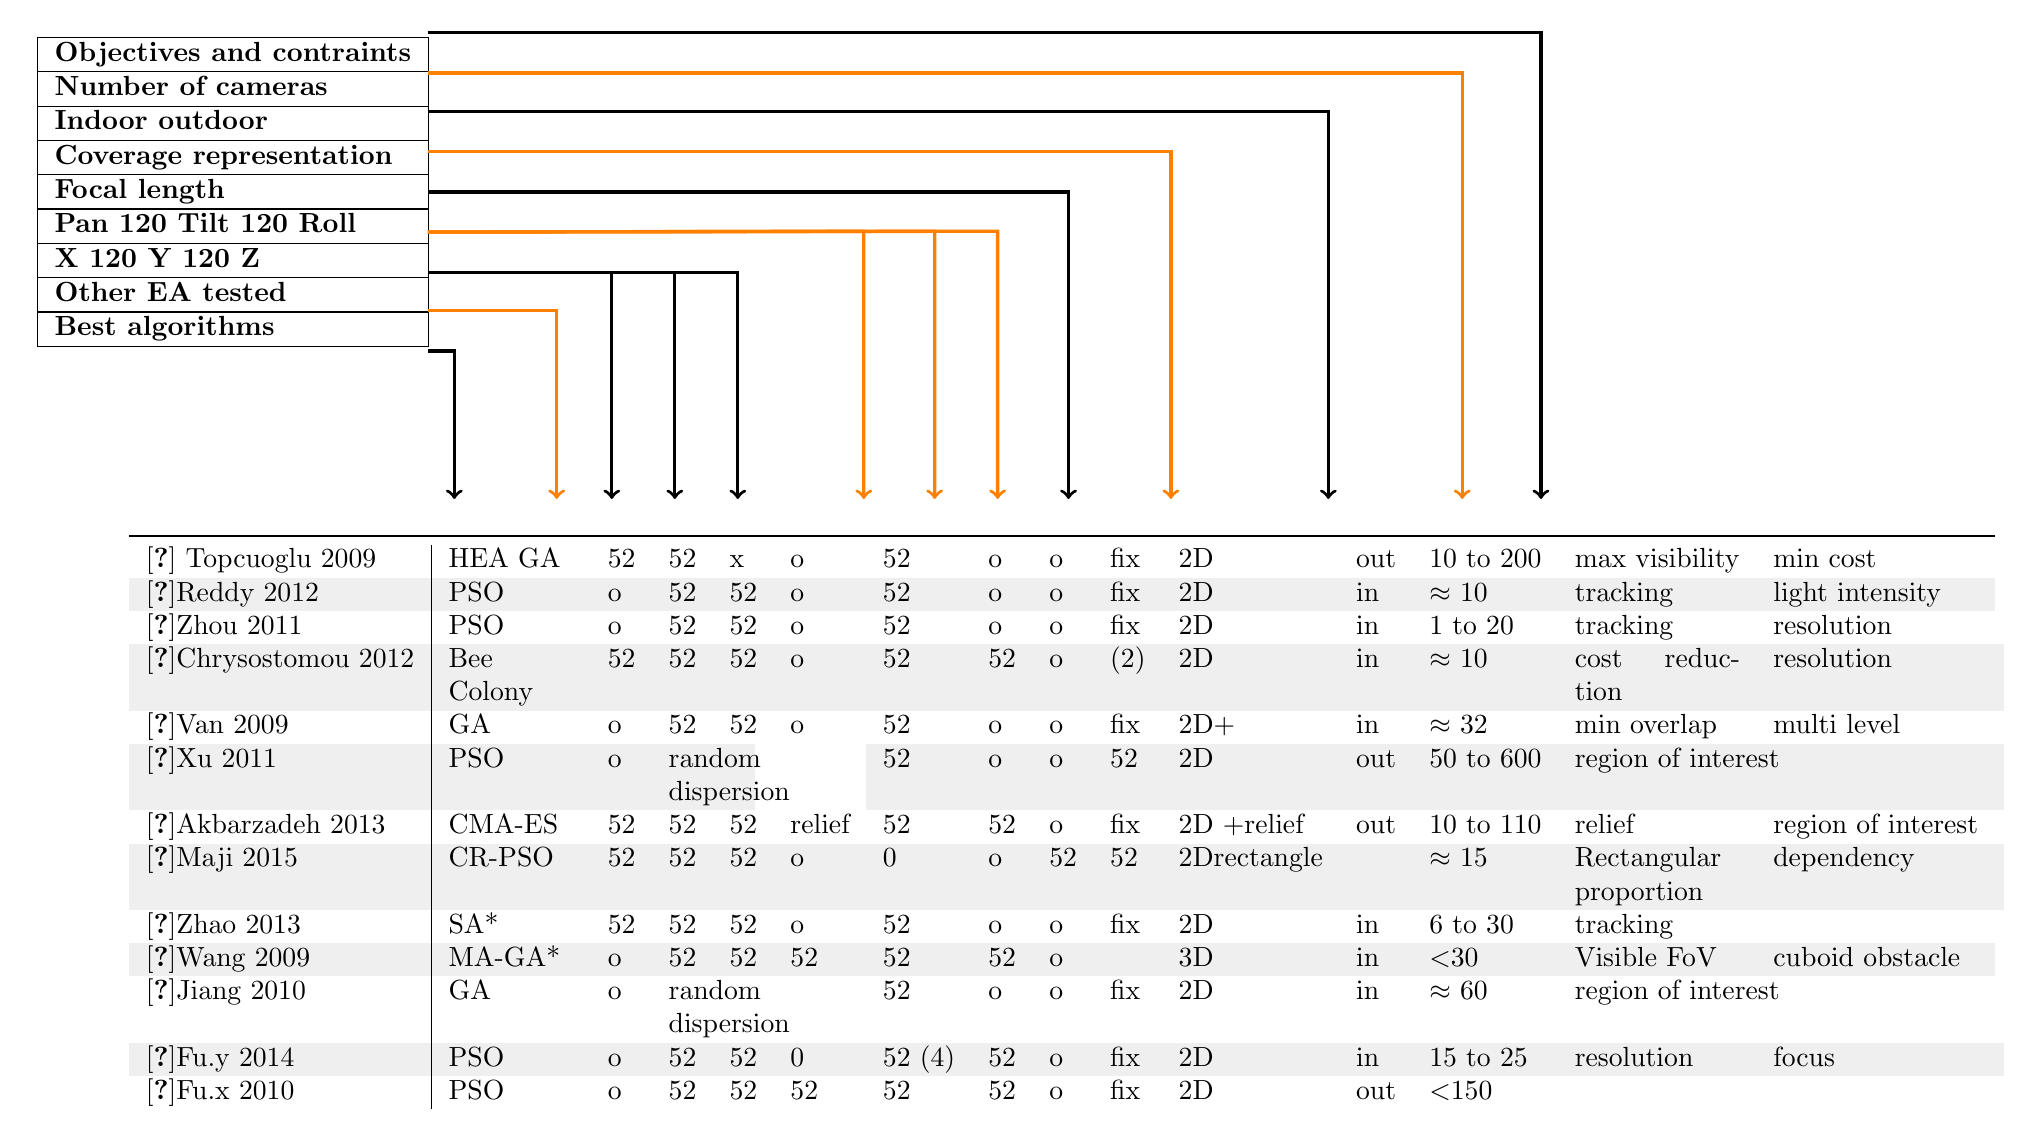
\begin{tikzpicture}[left]
\node (a) at (-0,-0)
{

\begin{tabular}{|l|}
\hline
 % \textbf{Reference} \\ \hline
%   \textbf{Best algorithms}   \\\hline %\vdots
%  \textbf{Other EA  tested}  \\\hline
%   \textbf{X \ding{120} Y \ding{120} Z}\\ \hline
%      \textbf{Pan \ding{120} Tilt \ding{120} Roll }\\ \hline
%         \textbf{Focal length }\\ \hline
%          \textbf{Coverage representation }\\ \hline
%          \textbf{Indoor outdoor }\\ \hline
%           \textbf{Number of cameras }\\ \hline
   \textbf{Objectives and contraints}  \\ \hline
    \textbf{Number of cameras }\\ \hline
    \textbf{Indoor outdoor }\\ \hline
    \textbf{Coverage representation }\\ \hline
    \textbf{Focal length }\\ \hline
    \textbf{Pan \ding{120} Tilt \ding{120} Roll }\\ \hline
    \textbf{X \ding{120} Y \ding{120} Z}\\ \hline 
    \textbf{Other EA  tested}  \\\hline   
    \textbf{Best algorithms}   \\\hline
\end{tabular}
};

\node[yshift=-5.91cm,xshift=22.5cm] (b) at (a.south) 
{
%%               ref  | soluce |EA soluc|x|y|z| pan | tilt |roll | focal |coverage|in out |nmb|
\begin{tabular}{@{} l|p{1.6cm}    l      l l l   l    l      l     l      l         l      l p{2.1cm}p{2.3cm} p{-0.9cm}@{}}
\toprule
\rowcolor[HTML]{F2F2F2} 
%\textbf{ref V2}                                      & \multicolumn{1}{l|}{\cellcolor[HTML]{F2F2F2}\textbf{\begin{tabular}[c]{@{}p{1.59cm}@{}}Best \\ solution\end{tabular}}} & \multicolumn{1}{l|}{\cellcolor[HTML]{F2F2F2}\begin{tabular}[c]{@{}p{0.9cm}@{}}Other\\ EA  \\ solution\end{tabular}} & \multicolumn{1}{l|}{\cellcolor[HTML]{F2F2F2}X} & \multicolumn{1}{l|}{\cellcolor[HTML]{F2F2F2}Y}& \multicolumn{1}{p{0.659cm}|}{\cellcolor[HTML]{F2F2F2}Z}&\multicolumn{1}{l|}{\cellcolor[HTML]{F2F2F2}Pan}& \multicolumn{1}{l|}{\cellcolor[HTML]{F2F2F2}Tilt}& \multicolumn{1}{l|}{\cellcolor[HTML]{F2F2F2}Roll}& \multicolumn{1}{p{1.119cm}|}{\cellcolor[HTML]{F2F2F2}Focal length} & \multicolumn{1}{l|}{\cellcolor[HTML]{F2F2F2}\begin{tabular}[c]{@{}p{1.55cm}@{}}Coverage\\  represen-tation\end{tabular}} & \multicolumn{1}{p{1.56cm}|}{\cellcolor[HTML]{F2F2F2}Indoor outdoor} & \multicolumn{1}{l|}{\cellcolor[HTML]{F2F2F2}\begin{tabular}[c]{@{}p{0.9cm}@{}}Number\\ of \\ cameras\end{tabular}} & \multicolumn{3}{l|}{\cellcolor[HTML]{F2F2F2}\begin{tabular}[c]{@{}l@{}}Secondary \\objectives \\ and contraints\end{tabular}}                                                                \\ \midrule
\rowcolor[HTML]{FFFFFF} 
\multicolumn{1}{l|}{\cellcolor[HTML]{FFFFFF}\cite{101*topcuoglu2009} Topcuoglu  2009} & HEA GA                                                                                                         &  \ding{52}                                                                     &  \ding{52} & x                                              & o                                              &  \ding{52}                                                & o                                                 & o                                                 & fix                                                       & 2D                                                                                                              & out                                                          & 10 to 200                                                                                                 & max visibility & min cost         &                    \\
\rowcolor[HTML]{EFEFEF} 
\multicolumn{1}{l|}{\cellcolor[HTML]{EFEFEF}\cite{33*reddy2012}Reddy 2012}  & PSO                                                                                                            & o                                                                     &  \ding{52} &  \ding{52}                                              & o                                              &  \ding{52}                                                & o                                                 & o                                                 & fix                                                       & 2D                                                                                                              & in                                                           & $\approx$ 10                                                                                              & tracking                                                                                                                    & \multicolumn{2}{l}{\cellcolor[HTML]{EFEFEF}light intensity}      \\
\rowcolor[HTML]{FFFFFF} 
\multicolumn{1}{l|}{\cellcolor[HTML]{FFFFFF}\cite{8*zhou2011}Zhou 2011}   & PSO                                                                                                            & o                                                                     &  \ding{52}                                              &  \ding{52}                                              & o                                              &  \ding{52} & o                                                 & o                                                 & fix                                                       & 2D                                                                                                              & in                                                           & 1 to 20                                                                                                   & tracking                                                                                                                    & resolution                    &                                  \\
\rowcolor[HTML]{EFEFEF} 
\multicolumn{1}{l|}{\cellcolor[HTML]{EFEFEF}\cite{82*chrysostomou2012}Chrysostomou 2012}  & Bee \newline Colony                                                                                                     &  \ding{52}                                                                     &  \ding{52}                                              &  \ding{52}                                              & o                                              &  \ding{52}                                                &  \ding{52}                                                 & o                                                 & (2)                                                  & 2D                                                                                                              & in                                                           & $\approx$ 10                                                                                              & cost reduction                                                                                                              & resolution                    &                                  \\
\rowcolor[HTML]{FFFFFF} 
\multicolumn{1}{l|}{\cellcolor[HTML]{FFFFFF}\cite{83*van2009}Van 2009}  & GA                                                                                                             & o                                                                     &  \ding{52}                                              &  \ding{52}                                              & o                                              &  \ding{52} & o                                                 & o                                                 & fix                                                       & 2D+                                                                                                             & in                                                           & $\approx$ 32                                                                                              & min overlap                                                                                                                 & multi level                   &                                 \\
\rowcolor[HTML]{EFEFEF} 
\multicolumn{1}{l|}{\cellcolor[HTML]{EFEFEF}\cite{84*xu2011}Xu 2011}  & PSO                                                                                                            & o                                                                     & \multicolumn{3}{p{0.89cm}}{\cellcolor[HTML]{EFEFEF}random \newline dispersion}                                                                                    &  \ding{52}                                                & o                                                 & o                                                 &  \ding{52}                                                         & 2D                                                                                                              & out                                                          & 50 to 600                                                                                                 & \multicolumn{2}{l}{\cellcolor[HTML]{EFEFEF}region of interest}                                                                                              &                                 \\
\rowcolor[HTML]{FFFFFF} 
\multicolumn{1}{l|}{\cellcolor[HTML]{FFFFFF}\cite{141*akbarzadeh2013}Akbarzadeh 2013} & CMA-ES                                                                                                         &  \ding{52}                                                                     &  \ding{52}                                              &  \ding{52}                                              & relief                                         &  \ding{52} &  \ding{52}                                                 & o                                                 & fix                                                       & 2D + \newline relief                                                                                                     & out                                                          & 10 to 110                                                                                                 & relief                                                                                                              & \multicolumn{2}{l}{\cellcolor[HTML]{FFFFFF}region of interest}   \\
\rowcolor[HTML]{EFEFEF} 
\multicolumn{1}{l|}{\cellcolor[HTML]{EFEFEF}\cite{143*maji2015}Maji 2015} & CR-PSO                                                                                                         &  \ding{52}                                                                     &  \ding{52}                                              &  \ding{52}                                              & o                                              & 0                                                & o                                                 &  \ding{52}                                                 &  \ding{52}                                                         & 2D \newline rectangle                                                                                                    &                                                              & $\approx$ 15                                                                                              & Rectangular proportion                                                                                                            & dependency                    &         \\
\rowcolor[HTML]{FFFFFF} 
\multicolumn{1}{l|}{\cellcolor[HTML]{FFFFFF}\cite{151*zhao2013}Zhao 2013} & SA*                                                                                                            &  \ding{52}                                                                     &  \ding{52}                                              &  \ding{52}                                              & o                                              &  \ding{52}                                                & o                                                 & o                                                 & fix                                                       & 2D                                                                                                              & in                                                           & 6 to 30                                                                                                   & tracking                                                                                                                    &                               &                                  \\
\rowcolor[HTML]{EFEFEF} 
\multicolumn{1}{l|}{\cellcolor[HTML]{EFEFEF}\cite{152*wang2009}Wang 2009} & MA-GA*                                                                                                         & o                                                                     &  \ding{52}                                              &  \ding{52}                                              &  \ding{52}                                              &  \ding{52}                                                &  \ding{52}                                                 & o                                                 &                                                           & 3D                                                                                                              & in                                                           & \textless30                                                                                               & Visible FoV                                                                                                                 & \multicolumn{2}{l}{\cellcolor[HTML]{EFEFEF}cuboid obstacle}      \\
\rowcolor[HTML]{FFFFFF} 
\multicolumn{1}{l|}{\cellcolor[HTML]{FFFFFF}\cite{165*jiang2010}Jiang 2010} & GA                                                                                                             & o                                                                     & \multicolumn{3}{p{0.659cm}}{\cellcolor[HTML]{FFFFFF}random  \newline dispersion}                                                                                    &  \ding{52}                                                & o                                                 & o                                                 & fix                                                       & 2D                                                                                                              & in                                                           & $\approx$ 60                                                                                              & \multicolumn{2}{l}{\cellcolor[HTML]{FFFFFF}region of interest}                                                                                              &                                  \\
\rowcolor[HTML]{EFEFEF} 
\multicolumn{1}{l|}{\cellcolor[HTML]{EFEFEF}\cite{193*fu2014}Fu.y 2014} & PSO                                                                                                            & o                                                                     &  \ding{52} &  \ding{52} & 0                                              &  \ding{52} (4)                                            &  \ding{52}                                                 & o                                                 & fix                                                       & 2D                                                                                                              & in                                                           & 15 to 25                                                                                                  & resolution                                                                                                                  & focus                         &                                 \\
\rowcolor[HTML]{FFFFFF} 
\multicolumn{1}{l|}{\cellcolor[HTML]{FFFFFF}\cite{194*fu2010}Fu.x 2010} & PSO                                                                                                            & o                                                                     &  \ding{52}                                              &  \ding{52}                                              &  \ding{52}                                              &  \ding{52}                                                &  \ding{52}                                                 & o                                                 & fix                                                       & 2D                                                                                                              & out                                                          & \textless150                                                                                              &                                                                                                                             &                               &                                 
\end{tabular} };
\draw [->,very thick] 		  (-0.135,2.02) -- (14,2.02) -- (14,-3.9); % constraint
\draw [->,very thick][orange] (-0.135,1.51) -- (13,1.51) -- (13,-3.9); % nmb cam
\draw [->,very thick] 		  (-0.135,1.02) -- (11.3,1.02) -- (11.3,-3.9); %in out
\draw [->,very thick][orange] (-0.135,0.51) -- (9.3,0.51) -- (9.3,-3.9);% coverage representation
\draw [->,very thick] 		  (-.135,0.0) -- (8,0) -- (8,-3.9); % focal lengh
\draw [->,very thick][orange] (-.135,-0.51) -- (7.1,-0.5) -- (7.1,-3.9); % roll
\draw [->,very thick][orange] (-.135,-0.51) -- (6.3,-0.5) -- (6.3,-3.9); % tilt
\draw [->,very thick][orange] (-.135,-0.51) -- (5.4,-0.5) -- (5.4,-3.9); % pan
\draw [->,very thick] 		  (-.135,-1.02) -- (3.8,-1.02) -- (3.8,-3.9);  %z
\draw [->,very thick] 		  (-.135,-1.02) -- (3.0,-1.02) -- (3.0,-3.9); % y
\draw [->,very thick]		  (-.135,-1.02) -- (2.2,-1.02) -- (2.2,-3.9); % x
\draw [->,very thick][orange] (-.135,-1.51) -- (1.5,-1.51) -- (1.5,-3.9); %EA tested
\draw [->,very thick] 		  (-.135,-2.02) -- (0.2,-2.02) -- (0.2,-3.9); % best Al
\end{tikzpicture}
\end{table} \label{tab:sum-upEA}
\end{landscape}



%%%%%%%%%%%%%%%%% exemple double  table arrow%%%%%%%%%%%%%%%%%%%%%%%%%%%%%%%%%%%%%

 
%%%%%%%%%%%%%%%%%%%%%%%%%%%%%%%%%%%%%%%%%%%%%%%%%%%%
%\subsection{Field of view}
%
% optical and the occlusion
%
%cover an area with certain amount of sensors. This number of position can be estimate as follow.\\   
%Each camera defined m focusing of optimize the solution and return a acceptable solution.
% 


%####################TODO############################
\section{Coverage path planning}\label{sec:CppLiterattur}

The coverage path planning  has for objective to design  the more efficient path to cover an area. The path has to cover all or  at least most of the area using  the shortest path. \\
The solutions highlighted in the literature until now was about placing numerous cameras or robotics cameras (as PTZ cameras and smart camera) for vast area composed by multiple obstacles.
The solutions proposed until now remains reliable only to monitor a vast area continuously with several cameras. 
The disadvantage of positioning a camera set appears quickly with the cost in computation time. The expensive cost is due to the several cameras and the communication network required to centralize the collected images. All the images must be collected in a real time. \\
In fact, in some applications, the area needs to be controlled periodically. The periodic control of the area does not require an installation for the set of fixed cameras. Until now the installation was composed by a set of immovable cameras unlike the solution presented in section see Section \ref{sec:SolutionBasedonEA} and \ref{sec:NonEAmethod}).
 The periodical control requirement can be illustrated with some example : the cartographies of the area is need just one time and can be completed with one fly over the area roughly bounded as in \citep{66*galceran2013,164*valente2013}, forest fire detection which requires a periodic fly over specific and vast region as in \cite{237*casbeer2006}, the hoovering robots which needs to cover all the room with possibility some on-line computation \citep{218*meiting2007,216*luo2002,215*lee2010,196*yang2004}  and the agriculture.
 About the agriculture application, a UAV needs to fly over the field few times in a year in order to control by photography the hydration, the maturity and anything else of the field as in \citep{164*valente2013,203*zarco2008,63*chao2008,105*long199,167*barrientos2011,177*lelong2008}. %\textbf{revoir les ref et trié un peu}.
For all these applications, the area must be covered but does not need a coverage of all the area instantly and continuously. The solution commonly proposed is the usage of only one sensor mounted on a mobile robot. The Mobile robot need to be adapted to the task and the environment, as flying  \citep{105*long1991}, driving \citep{30*bodor2005,213*roberts2008}, swimming \cite{66*galceran2013}.\\
 The mobile robot with the sensor moves in the space to cover all the area. In this case, the objective is to determine the best path for the mobile robot to cover  the area. The best path is dependent on the constraint of each problem. However, the common point in theses papers is to obtain the shorter path.
The following section is focused on finding the best Coverage Path Planing (CPP) for a sensor mounted on a mobile robot. 
In most cases,  the sensor is a perspective camera. To estimate the best CPP, different algorithms and methodologies have been applied in the literature to solve various problems.

  The following sections are focused on the different algorithms and methodologies applied to optimize the CPP problem. First, the watchman route problem is introduced to highlight the origin of the CPP problem and the relation with the cameras positioning for optimal coverage. In a second time, the more popular solutions are discussed.
 
%hovering robot
% In some case some domestic robots as  the hovering robot   or similar  must also to 213*


%-------------------------------------\\
% Grenzdorffer, G., Engel, A., Teichert, B.: The photogram-metric potential of low-cost UAVs in forestry and agriculture. Int. Arch. Photogram. Rem. Sens. Spatial Inform. Sci.
%31(B3), 1207–1214 (2008) 
%
%Zarco-Tejada, P.J., Berni, J.A., Suarez, L., Fereres, E.: A new era in remote sensing of crops with unmanned robots.
%SPIE Newsroom, pp. 2–4 (2008)
%
%Kazmi, W., Bisgaard, M., Garcia-Ruiz, F., Hansen, K.D.,
%la Cour-Harbo, A.: Adaptive surveying and early treatment
%of crops with a team of autonomous vehicles. In: European
%Conference on Mobile Robots, pp. 253–258 (2011) 


\subsection{AGP  to watchman route problem}\label{sec:WRP}


Before exploring the solutions proposed for the CPP, it is essential to understand the role of the Watchman Route Problem (WRP). The WRP is closely related to the CPP and the WRP has impacted the research about the CPP. 
The following sections are focused on the definition of the WRP, the proposed solutions in order to solve it, and finally, a brief discussion is drawn about the WRP .
 
\subsubsection{Definition of the watchmen route problem }

 \begin{mfigures}[!]
{Watchman route problem answer illustration. }{fig:WRPillust} \centering
\mfigure{width=.4\linewidth}{img/WRPillustration.png}{}{subfig:WRPi}
\hspace{1cm}
\end{mfigures}	
The Watchman Route Problem is introduced for the first time by Chin and Ntafos in 1987 \cite{54*chin1988}. The problem of the WRP can be summarized in one sentence :

\textbf{"How to calculate a shortest route contained inside a polygon such that any points inside this polygon is visible from at least one point of the route?"}.  

The guard has to cover an area represented by a polygon (see the illustration of the problems in Figure \figref{fig:WRPillust}). The guard is considered as \textit{perfect} with no restriction in the field of view (the guard can see at $360^\circ$) and no restriction in the depth field (the guard can see from on extremity of the room to another. The guard can see the opposite wall excepted if an obstacle occludes the view). The guard abilities are directly inspired by the AGP (see \ref{sec:AGP})
The shape of the polygon is primordial and affect greatly the possible solutions and the complexity to solve the WRP.
The WRP problem is by many aspects closely related to the AGP. The AGP (see Section \ref{sec:AGP}) is commonly considered as the root of the WRP.
 In fact, the WRP is not only focused on standing position, but on finding an optimal path. The path has to be optimized to cover all the points which compose the polygon  and the path has to be as shorter as possible.
 
% A common way to build a path with as to cover a polygon can be to search the waypoints  which compose the path. Once the waypoints found the next step is to compute a path passing by all the previously founded waypoints. 
 The next section will introduce the possible methods and algorithms applicable to solve or atleast optimize a solution for a WRP.
 


%polygone impact on the complexity
%AGP -> WRP  

% source : An Approximate Algorithm for Solving the Watchman Route Problem Fajie Li and Reinhard Klette
 
\subsubsection{Solutions} 

The WRP problem can be solved under some conditions. The solutions to solve it are applicable only if the polygon is simple. A polygon is considered as simple, when the boundary of it are composed of continue straight lines that do not intersect between them. To close this definition, it is important to precise the simple polygon does not have any hole (see Figure \figref{fig:simplePoly}). 
 \begin{mfigures}[!]
{Few examples to illustrate the simple polygon shape. }{fig:simplePoly} \centering
\mfigure{width=.4\linewidth}{img/SimplPolygonA.png}{Example of simple polygons.}{subfig:SimplePoly}
\hspace{1cm}
\mfigure{width=.4\linewidth}{img/SimplPolygonB.png}{Example of complex polygons.}{subfig:nonSimplePoly}
\hspace{1cm}
\end{mfigures}	

To solve the WRP, few algorithms were developed. The algorithms proposed in the literature enables  successively better algorithm  to solve the problem. The first interesting algorithm for the WRP with a simple polygon is the early work of Tan et al \cite{234*tan2001}. Tan et al.\citep{234*tan2001}  proposed an algorithm for a fast computation time. The solution proposed works with a simple polygon composed by $n$ vertices and its complexity belongs to polynomial time $O(n^5)$. \\
Others contribution about WRP were then proposed. Dror et al. \cite{233*dror2003} proposed a better time complexity. In fact, in \cite{233*dror2003}, the considered solution with a simple polygon is working in $O(n^3 log n)$ complexity.  The deterministic solution applied is also usable in closely related problems of the WRT as the zoo-keeper problem and safari problem which makes this contribution versatile and generic.
Two other algorithms \citep{234*tan2001,233*dror2003}, are usable only in the case of simple polygons to deliver the optimal solution which is the shortest path for a full room coverage. 

To have a more general solutions for WRP, the proposition lie in having an efficient algorithm working also with complex polygons. A possible solution could be to look for an efficient approximation by optimizing the position of the guards and their respective paths. An efficient approximation means a path acceptably short. In fact the path computed can not be certified as the "best path" but only as the shorter found.

Several efficient approximations have been proposed such as in \citep{235*faigl2010} and \citep{53*packer2008}. 

In Packer \citep{53*packer2008},  the algorithm proposed is based on splitting the problem into two sub-problems. The first sub-problem consider the search of a set of points which can be good enough to cover all the area despite a restricted visibility range. These points are called waypoints.  
Once the set of waypoints to cover all the polygons are found, the second sub-problem consider the creation of a path passing by all these points. 
 This second sub-problem is similar to a classic Travelling Salesman Problem (TSP). The TSP tries to answer the questions asked by a travelling salesman "\textbf{What is the shortest path passing by each city only one time and return to the starting city?}".
  In the TSP, the cities are the nodes on the interconnected map and the roads are the connections between them. The TSP is a well known NP-hard and NP-complete problem when applied in  some conditions, as described in \citep{236*karp1972}. \\ 
Finally the solution used for the TSP can be applied for the second sub-problem of WRT.
Subsequently, TSP can be applied for the second sub-problem of WRT solution proposed by Packer \citep{53*packer2008}.

%a similar method than the one proposed by faigl in [235*] has been proposed to approximate the shorter path as possible. To approximate the shorter path the problem of WRP is also split in two sub-problem. The first sub-problem is considered as similar then the AGP and use the method form AGP to find the waypoints. The second sub-problem is also compared as TSP.

In Faigl  \citep{235*faigl2010}  a similar method to the one proposed by Packer \citep{53*packer2008} has been proposed to approximate the shorter path. The problem is also split into two sub-problems. The first is to optimize the position of the waypoints and the second is to schedule the position in order to create a path planning (directly inspired by the TSP). 
%the algorithm proposed is based on splitting the problem into two sub-problems. The first sub-problem is to find a set of point with can be good enough to cover all the area despite a restricted visibility range. These points are called waypoints for the following sections. 
 Furthermore, the solution proposed by Faigl in \citep{235*faigl2010} is applicable to a watchman with a restricted visibility range i.e. equivalent to a $360^\circ$ field of view with a \textit{restricted depth of field}. This restriction affects greatly the waypoints positioning. Due to this constraint, more waypoints needs to be placed to cover an area.
 Once the set of waypoints for the polygon coverage is found, the second sub-problem is to create a path passing by all these waypoints.  The algorithms proposed  to perform such task are also inspired by the solution given for the optimization of the TSP.
 %This second sub-problem is similar then a classic Travelling Salesman Problem (TSP). The TSP  try to answer the question ask by a travelling salesman "What is the shortest path passing by each city only one time and return to the starting city?". In the TSP, the city are the node on the interconnected map with the road as the connexion. The TSP is well known as NP-hard and NP-complete in some condition as described in [236*]. \\ 
%Finally the solution used for the TSP can be applied for the second sub-problem of WRT.
% The TSP and the algorithms proposed to optimize it are discussed more in detail later \ref{par:TSPPathPlan} \\
%In Packer [53*] similar solution than the one proposed by faigl in [235*] has been proposed to approximate the shorter path as possible. To approximate the shorter path the problem of WRP is also split in two sub-problem. The first sub-problem is considered as similar then the AGP and use the method form AGP to find the waypoints position. When the  waypoints are placed in the polygon the second sub-problem which is to schedule the waypoints to have a shorter path as possible. 



%from https://link.springer.com/content/pdf/10.1007%2F978-3-642-31155-0.pdf
%compexity $O(n^4 log n)$ :\\
%Dror, M., Efrat, A., Lubiw, A., Mitchell, J.S.B.: Touring a sequence of polygons.
%In: Proc. 35th Symposium on Theory of Computing, pp. 473–482 (2003)\\
%Tan, X.: Fast computation of shortest watchman routes in simple polygons. Information Processing Letters 77(1), 27–33 (2001) \\ 

%linear approximation :  Tan, X.: A linear-time 2-approximation algorithm for the watchman route problem for simple polygons. Theoretical Computer Science 384(1), 92–103 (2007)

%Polygons with holes the problem is NP-hard : 54*\\
 %  Dumitrescu, A., T oth, C.D.:Watchman tours for polygons with holes. Computational Geometry: Theory and Applications  (2012)

 %An $O (log n)-approximation$ for Rectilinear polygons are also known as orthogonal polygons.:Mata, C.S., Mitchell, J.S.B.: Approximation algorithms for geometric tour and network design problems. In: Proc. 11th Symposium on Computational Geometry, pp. 360–369 (1995)

\subsubsection{Limit and consequences}

The methods proposed to solve the WRP are really interesting and gives a good solution in some specific conditions. These conditions make his methods special cases.
 In fact the optimal solution, i.e. the shortest path which covers all the area (polygon), are usable only if the polygons observe some rules. The polygon must be simple and take into account the guard ability (no viewing constraints).  \\
When the polygon is more complex, the optimal solution cannot be reached. The methods applied to solve the WRP for complex area are promising. Especially the problem splitting into sub-problems. Despite this interesting aspect, the solutions proposed are most of the time limited due to the area representation. This representation associated to the geometric methodologies to find the waypoints gives a crucial importance to the number of vertices inducing also the number of cameras. \\
A large  number of vertices imply  consequently that the first sub-problem may be difficult and time-consuming to solve.
Consequently this method is not the more appropriate for vast and complex outdoor areas which would require  numerous vertices to describe.
 The biggest limit of the WRP is the ability of the watchmen. Indeed, in the original problem, the watchmen are considered having a perfect visibility. The solution proposed solving the WRP are not usable with the accumulation of new visibility constraints. 
In Faigl \citep{235*faigl2010}, the WRP started to be extended by adding a constraint on the visibility. In this condition the problem is slightly modified to shift from self-organizing map to  coverage path planning. But despite this addition of a restricted  depth of field, the proposed solution based on geometric heuristic do not allows the accumulation of more constraints.

The AGP then WRP extensively impacted the vision, the design of cameras coverage problem  and coverage path planning field.  Among the solutions discussed in the previous section, numerous articles are based and/or refers to the AGP and WRP. Our work is consequently inspired by those formulations and will propose to extend it.



 


%tout comme l'agp a était une source d'inspiration pour  le positionnement de camera  le wmp est lui aussi une source d'inspiration pour  le cpp 
%The CPP 
%The origin of CPP can be found on the Watch Men Problem (WMP). The next
%
%The Watch Men Problem (WMP) is directly derived form the AGP. 
%
%As the importance of AGP for the problem of camera positioning  the Watch men problem 
%53* parcker eli :  propose a solution  to solve the watchmen problem based on the result optianined by the AGP \\ 
%54* Chin : complexity proof of NP-hard  for the watchmen problem by reduction of TSP + article fondateur
%

\subsection{CPP solutions}



To optimize the CPP problems many solutions were proposed. The different algorithms and methodologies proposed are discussed in the following sections. The methodologies proposed can be organized in several branches. 
The most important branch to optimize the CPP corresponds to the usage of sweep associate to a cellular decomposition.
%60* =  une découpe en zone  rectangle et utilisation  de la triangulation pour le positionment de waypoint  puit tsp.
%
%217*= utilisation du GA  pour la conexion entre polygone simple (1er étape découpe de la zone  en  polygone en fonction des obstacle - 2e  crée un graphe qui  reli les différant sous partie ( polygone) GA  -3 choisir le sweep le plus )
%
%61* 62*= floor planning

\subsubsection{Cellular decomposition and sweep} \label{sec:CPPcellDecompSol}
\begin{mfigures}[!]{Illustration  of  simple cell decomposition with sweep.}{fig:CellDecp} \centering
\mfigure{width=.4\linewidth}{img/CellDecop.png}{}{}

\end{mfigures}	
To solve the CPP problem, the most common solution is considered to be the cellular decomposition. The cellular decomposition is by some aspects inspired by the methodologies presented in the WRP.
To recall one of the interesting solution for the WRP, the methodology starts by splitting the problem in two sub-problems and optimize those independently. The first sub-problem solve the search of the best waypoints and the second sub-problem corresponds to finding the shortest path passing by all the waypoints (like the TSP).
 The Cellular decomposition also split the problem of CPP in two sub-problems. The first sub-problem is focus on the decomposition of the complex area in several cells. Each cell has to be a simple polygon (basically a rectangle or latter any quadrilateral polygon). Inside each cell a sweeping has be applied in order to cover all the area (see Figure \figref{fig:CellDecp}). The second sub-problem is to find the path which can connect each simple polygon. The problem has to take in account, the sweep start and end to find the global optimized shorter path. Where the global optimized shorter path take in account the sweep trajectory of each simple polygon and the path between the simple polygons.
 
 Finally the cellular decomposition is made by decomposing the complex area, choosing the appropriate sweep and finding the shortest path to connect the cells. 
 
 \paragraph*{Decomposition}\label{par:decomposition}

 The decomposition in cells has for objective to split a complex area in several sub-areas. Each sub-area has to be simple in term of shape in order to apply a sweep. 
Since the 90s, numerous algorithms have been developed for the cellular decomposition. Among the algorithms for cellular decomposition, 3 types of decomposition were deduced as shown in the survey of Choset  \cite{214*choset2001} and  Galceran and al \cite{66*galceran2013}. 
\begin{itemize}
	\item Approximate: 
		An approximate decomposition is based on discretization of the area. The free space of the area is represented by a set of cases (grid). Each case of the grid has to be covered by a mobile robot. A case is considered completely covered if the robot is on the associated position. Which means that the frequency of the grid is defined by the covered area of the mobile robot. 
		The approximate decomposition by cases is convenient to describe the area but is greatly limited due to the low sampling frequency of the gird and the limited amount of possible trajectories.\\
	 
	\item Semi approximate: 
	 \begin{mfigures}[!]
{Illustration of a semi approximate decomposition outcome from the survey  of Choset \citep{214*choset2001}. The 4 figures illustrates the trajectory of the robot over the time.}{fig:choset214SemiAprox} \centering
\mfigure{width=.95\linewidth}{img/Choset214SemiDecomp.png}{}{subfig:WRPi}
\hspace{1cm}
\end{mfigures}	
 The semi approximate decomposition is partly based on the discretization of the space. The idea is to create a set of large cells. The width of the cells is fixed and the height is relative to the area boundaries (see in \citep{214*choset2001}). 
	 The semi approximate cell decomposition allows to have cells with two parallel sides with a fixed size (right and left) and  the  two other sides adapted to the boundaries (up and down. See the illustration  of a semi approximation in Figure \figref{fig:choset214SemiAprox}).  The width  of  the cells are chosen accordingly to half of the focal length of the camera mounted on the mobile robot. The area is covered by following the boundaries of the cells with sweep to cover cells  after cells.
	 The advantage of the semi approximate decomposition is the ease to describe a vast area and the low computation time required. Additionally, this decomposition can be made on-line by the robot and do not requires a high level of knowledge of the area. 
	 The disadvantage is the non-optimization of path due to the cells decomposition. The simplicity  of this decomposition  can generate case where the robot have to cover many times the same place. The semi approximate cellular decomposition do not allow to have a well optimized path planning. \\
	 
	 %%%%% add fig from238* fig8 to --> from214
	\item Exact cellular decomposition: 
	The exact cellular decomposition describe the area by creating juxtaposed geometrical regions. The size of the regions (or cells) are not depending on the robot ability contrarily to the previous decomposition. The large size of the cells allows the  mobile robot to do back and forth motion to cover all the cells (also called sweep as in Figure \figref{fig:sweepSpiral}).  The cells have to be ordered to conserve an efficient and short path going through all the cells. 
The global path distance have to be reduced by an appropriation of the path passing through cells.
	The exact cellular decomposition became popular and numerous algorithms have been proposed. The proposed algorithms  can be a faster decomposition or a deduction of more appropriate shape depending on the basic rectangular cells. 
	Among the numerous exact cellular decomposition propositions: the trapezoidal decomposition for its simplicity and historic importance, the Boustrophedon decomposition  and  Morse-based Cellular Decomposition can be cited for their importance in the construction of other exact cellular decomposition. These algorithms and other are clearly summarized in the survey of Carreras and Galceran \citep{66*galceran2013}. 
	The exact cellular decomposition has been still studied since the survey of  Carreras and Galceran  \citep{66*galceran2013} and upgraded, as in \cite{144*torres2016}, proposing a decomposition for concave or multiple polygons.
	
\end{itemize}




% survey = 66* 214*
% CPP experimentation (164* 167*)
% 
%119* 214* 215* 146*  144* 164* 167* 190*=cellule decomposition \\ 

 
 \paragraph*{Sweeps} \label{par:sweep}
	The back and forth or sweep is an essential element of the CPP by cellular decomposition. The sweep has to cover the entirety of the cells. The cells are splitting the area in relatively simple polygons (as shown in the paragraph \ref{par:decomposition} and  the Figure \figref{fig:CellDecp}). The sweep needs to be adapted to the shape of the cells and also must start and finish in a appropriate position taking into consideration the path to the next cells.
	For that the starting point and the ending point of the sweep are crucial for the global path planning.
	In Torres et al. \cite{144*torres2016},  the sweep is function of a direction and can go clockwise or counter-clockwise to have a start and end in the appropriate position for the transition. 
	 This enables to have 8 different applicable sweeps at each cells depending on the most appropriate start and finish; according to the computed path. The sweeps are adapted depending on : 
	 \begin{itemize}
	 \item The turn sides ( clockwise or counter-clockwise)
	 \item The directions (horizontal or vertical)
	 \item The finishing  positions (start and stop from the same side or opposite side)
\end{itemize}	
	 The sweep can be also alternatively switched for a spiral as proposed in Jimenez et al. \citep{217*jimenez2007}. The proposed sweep and spiral  are adaptable depending on the context. The sweep can have two directions and for the spiral two turn sides (clockwise or counter-clockwise).  The different sweeps and spirals are illustrated in the Figure \figref{fig:sweepSpiral}. 
	  \begin{mfigures}[!]{Illustration of the different sweeps and spirals.}{fig:sweepSpiral} \centering
\mfigure{width=.55\linewidth}{img/SweepSpiral.png}{}{}
\end{mfigures} 

	To have an adapted sweep, the footprint has to be defined depending on the camera ability and the objectives. In \cite{144*torres2016}, the size of the sweep is dependent on the area covered by a camera and a considered sufficient amount of overlaps for the 3D reconstruction (see also\citep{191*di2016}). In Li et al.  \citep{146*li2011}, the footprint of the camera with a small pan is considered. Due to the pan, the camera projection is not a rectangle but a trapezoid. Consequently the sweep size is adapted by taking the larger side of the trapezoid for the sweep dimension.
	Also for the grid decomposition, the sweep size is directly related to the coverage ability of the mobile robot (as example in \citep{215*lee2010,195*choi2009}).  % also 216*+48  215*  195* +55 218*+12  use a sensing camera at the front).
	
	One extra element necessary for the sweep can be in some cases the external element such as the wind. In \citep{215*lee2010,190*hsu2014},  %!![190*] !! 
	the external condition are taken into account in the cost function and it influence the sweep.
	
	
	To summarizes the sweeps requires to be adapted to the area and the relation between cells. To choose the appropriate sweeps the following element have to be considered:
	\begin{itemize}
		\item The size of sweep  have to be defined depending on the ability of the camera (footprint size).
		\item The direction (horizontal or vertical).
		\item The  starting and finishing  position (start and stop from the same side or opposite side)
	\end{itemize}
To  obtain the more appropriate sweep, it is primordial to know before the cells scheduling. The cells scheduling are a crucial part of the path planning.

	% The foot print, 
	 %the type of sweep ( sweep or spiral), the direction (horizontal or vertical), the finishing  position (start and stop form the same side or opposite side) the size of the footprint has to be defined depending then the ability of the camera. 
	
	%215* 190* generic cost depending then external condition  and  using spiral or sweep
	 
	 %144*  size to the sweep adapted  depending then the footprint of the camera on the ground floor  with propose lot of overlap useful for the 3D reconstruction.  the sweep  is function then a direction  and can go  clockwise or counter-clockwise to have  a start and end in the appropriate position for the transition. 
	 %This allow to have 8 different sweep applicable at each cell depending then the more apropriate start and finish depending  then the turn side ( clockwise or counter-clockwise), the direction (horizontal or vertical)  and the finishing ( start and stop form the same side or opposite side).  
	% 217*  propose  sweep and spiral with  different direction  for the sweep and two turn side for the  spiral

	%195* spiral sweeping for on-line coverage (for hoover application)
	 
%	209* comparative between cellular decomposition with sweep and a global spiral on the complex shape. (master these)
	
	
    
 
 %décompostion celulurai avec étude sur le remplisage sweep ou  spyrale pour  des zone concave our convex 
%Ost, G.: Search Path Generation with UAV Applications Using Approximate Convex Decomposition, Masters Thesis. Linkopings universitet, Sweden (2012)

 
 \paragraph*{Path planning} \label{par:TSPPathPlan}
 
The aim of the path planning is to find the short path going through all the cells. Finding the best path planning passing by all the waypoints or in this case all the cells, is a complex problem  which can be formulated as a TSP. The path planning became even more complex in the case of exact cellular decomposition or for any decomposition which requires a sweeping inside each cells. Indeed, in this case, the goal is to have the shortest path planning with taking into account each sweep and transition between cells. In the previous paragraph \ref{par:sweep}, the different sweeps and spirals have been detailed. The start and the end of the sweep are the crucial elements to consider during the path planning computation.
 Obviously, to find the best scheduling between each cells, the algorithm induces by the TSP are commonly used.     
 
 When the area is decomposed in cells, the goal is to schedule the right-of-way from one cell to another in order to create an efficient path. The scheduling of the cells can be optimized by using the paradigm of TSP with the same algorithms to have an acceptable path planning. 
The TSP is a well known problem and is deeply studied from long time ago. First is essential  to remember the TSP is an NP-complete and NP-hard problem as prooved in Karp in \cite{236*karp1972}. 

To optimize the TSP, numerous algorithms have been tested and some of them have been specially applied to schedule the cells to have the shortest path. In  An et al. \cite{60*an2013}, two algorithms were tested before developping a third. The algorithms used are based on branch and bound. The algorithm developed in \cite{60*an2013} is called Novel Previous-Next Waypoints Coverage Constraint (PNWCC). The algorithms presented in \cite{60*an2013} proposes at same time a schedule of each cells as well as a smooth trajectory without sharp edges usable for non holonomic driving robots. 

In the survey of Carreras et Galceran \citep{66*galceran2013}, the solutions proposed to solve the TSP are asked to compute an exhaustive walk trough the adjacency graph. These solutions are workable only for computingg small adjacency graph. The GA is popular to optimize the TSP and is commonly used to evaluate the influence of parameters as in \citep{68*muhlenbein1989} \citep{80*serpell2010}. About the CPP problem, the GA is also used to optimize the TSP part as in Jimenez et al. \citep{217*jimenez2007}, where the GA is applied to find an optimized schedule retrospectively of an exact cellular decomposition of a complex polygon. \\
The GA is announced to be appropriated to obtain an optimized solution for the TSP. 
In some situations, a  TSP is not realistic and some external constraints can be added such as the wind effect, turbulence, or holonomy constraint as in \citep{56*davies2006,102*ware2016,66*galceran2013}). The addition of external constraints may leads to more complex scheduling  of the cells. 
 
 
%236* proof of NP complet and NP-hard

%60* use of TSP = any TSP algorithm can be used  as the branch and bound algorithm. or best choice is to use  the Hearest Neighbor algorithm  and finally propose a Novel PNWCC solution with propose a path without  sharp edges usable for non holonomic driving robots.
%66* TSP  solver with a  several methode. 
%217* use of TSP  solved with GA (CPP)217*  GA  for the TSP

%102* TSP with external constraint (wind)
 
%68* asyncorne parallel GA for TSP
%80* GA mutation rate for TSP 
%139* GA config for TSP
%172* TSP GA   Use of GA multi goal for  schedule the charge on  m machine and n job  

%XX 56* evitement d'obstacle et trachectioire 
%XXX 214* reference of the problem 
%XXX 164*  use TSP 


%%%%%\subsubsection{Other solution for CPP}
%%%%%	216* 218* 215* 196*= robot roulant hoover \\
%%%%%	
%%%%%	191* 190* 211* 212* = low enregie cpp\\
%
%In choset et al 214*  some heuristic and randomized solution has been presented.    
%one of the basic heuristic is to follow the boundary of the area to cover. (R.A. Brooks, A robust layered control system for a mobile robot, IEEE J. Robotics Autom. (1986)   et
%  E. Gat and G. Dorais, Robot navigation by conditional sequencing, in: Proc. IEEE Int. Conf. on
%Robotics and Automation, San Diego, CA (May 1994) pp. 1293–1299. )
%
%	\begin{itemize}
%	\item Liu, Y., Lin, X., Zhu, S.: Combined coverage path planning for autonomous cleaning robots in unstructured environments. In: Proc. World Congress on Intelligent Control and Autom., pp. 8271–8276 (2008) 
%
%	\item Luo, C., Yang, S.X.: A bioinspired neural network for
%real-time concurrent map building and complete coverage robot navigation in unknown environments. IEEE
%Trans. Neural Netw. 19(7), 1279–1298 (2008) == PDF TNN2008  cite 132  neural network pour  robot aspirateur  avec construction de la map  et complet couverture  
%	
%	\item Oh, J.S., Choi, Y.H., Park, J.B., Zheng, Y.F.: Complete coverage navigation of cleaning robots using
%triangular-cell-based map. IEEE Trans. Ind. Electron. 51(3), 718–726 (2004) == pdf navigation-robot.pdf   robot roulant construction de son univer ajout de direction possible
%
%	\item 214* = propose 2 heuristic  et randomize 
%	\end{itemize}
	
	
%	177*= multi spectral\\
%	119* 214* 215* 146* 66* 144* 164* 167* 190*=cellule decomposition \\
%	146* 147* = optimization de trajectoire local cpp\\
%	196* =neural Network \\
%	195* 189*= ???
%
%%\subsubsection{ ??sensor positioned in electronic circuit ??}
%%\subsection{Robot application}
%	%\subsubsection{hover robot}
%	%\subsubsection{submarine}
%	
%	
%	!!!!!!!!!!!!!!!!!!!!!!resource!!!!!!!!!!!!!!!!!!!!!!!!!!!!\\ 
%	from 190
%
%\subparagraph{Probelm du CPP par Genetic Algo GA }	
%\begin{itemize}
%	\item Jimenez, P.A., Shirnzadeh, B., Nicholson, A., Alici, G.: Optimal area covering using genetic algorithms. In: Proc. IEEE/ASME Int. Conf. Advanced Intelligent Mechatronics, pp. 1–5 (2007)
%	
%	\item Wang, M., Tan, S., Yan, L.: Complete coverage path planning of wall-cleaning robot using visual sensor. In: Proc. Int. Conf. Electronic Measurement and
%Instruments, pp. 159–164 (2007)
%
%	\item Zhang, G., Ferrari, S., Qian, M.: An information
%roadmap method for robotic sensor path planning. J. Intell. Robot. Syst. 56(1–2), 69–98 (2009)
%	\end{itemize}
%
%
%\subparagraph{CPP  résolution par  neural Network pour certain une gestion dinamique de obstacle  }	
%\begin{itemize}
%	\item Lee, T.K., Baek, S.H., Oh, S.Y., Choi, Y.H.: Complete coverage algorithm based on linked smooth spiral paths for mobile robots. In: Proc. Int. Conf. Control, Automation, Robotics and Vision, pp. 609–614 (2010)
%
%	
%	\item Yang, S.X., Luo, C.: A neural network approach to complete coverage path planning. IEEE Trans. Syst. Man Cybern. 34(1), 718–725 (2004)
%
%
%
%	\item Luo, C., Yang, S.X., Stacey, D.A., Jofriet, J.C.: A solution to vicinity problem of obstacles in complete coverage path planning. In: Proc. IEEE Int. Conf. Robotics
%and Automation, pp. 612–617 (2002)
%
%\item Qiu, X., Song, J., Zhang, X., Liu, S.: A complete coverage path planning method for mobile robot in uncertain environments. In: Proc. World Congress on
%Intelligent Control and Automation, pp. 8892–8896 (2006)
%
%
%\item Qiu, X., Liu, S., Yang, S.X.: A rolling method for 
%complete coverage path planning in uncertain environments. In: Proc. IEEE Int. Conf. Robotics and
%Biomimetics, pp. 146–151 (2004)
%
%\item Luo, C., Yang, S.X., Stacey, D.A.: Real-time path planning with deadlock avoidance of multiple cleaning
%robots. In: Proc. IEEE Int. Conf. Robotics and Automation, pp. 4080–4085 (2003) 
%
%	\end{itemize}
%
%\subparagraph{survey  sur la décomposition  linaire }
%	\begin{itemize}
%	\item Choset, H.: Coverage for robotics-a survey of recent results. Ann. Math. Artif. Intell. 31, 113–126 (2001)
%	
%	\end{itemize}
%	
%	\paragraph{66*  points clé}
%	coverage path planning in the 3D space (UAV and Subamrine)\\ 
%	cellular decomposition :  requantangle cellul  ;  trapezoidal decomposition ; Boustrophedon Decomposition; Morse-based Cellular Decomposition ; online Morse-based Boustrophedon Decomposition ; Landmark-based Topological; slice Decomposition ;On-line Topological Coverage Algorithm ;Contact Sensor-based Coverage of Rectilinear Environments;Grid-based Methods;Grid-based Coverage using the Wavefront Algorithm;Neural Network-based Coverage on Grid Maps
%Coverage 
%		\paragraph{214* choset}
%		heurisitc and randomized approche :  propose a solution  on multi robot repultion system to spread the  robot  in the space and  use   a random motion  as strategie to explore the area[5,27]. \\(T. Balch and R.C. Arkin, Communication in reactive multiagent robotic systems, Autonom. Robots 1995) , unknown obstacles of arbitrary shape, Algorithmica 2 (1987) 403–430. ;:;\\ D. MacKenzie and T. Balch, Making a clean sweep: Behavior based vacuuming, in: AAAI Fall Symposium, Instationating Real-World Agents (1996). )
%		
%		\paragraph{Semi-approximate}
%		Hert and Lumelsky : propose a system based on cell decomposition  and   boundary folowing 
%		
%		\paragraph{multi robots}
		
		\subsubsection{Other solutions}
		
		Among the algorithms developed for the CPP, some interesting methods have to be studied.		
		Some algorithms has been discussed in Choset \cite{214*choset2001} as approximate solution (see Section \ref{par:decomposition}). 
		
%	!!!	Despite this classification the decomposition of the area is not the really effective and the algorithms used must be highlight. Among it the solution based on regular grid discretization which this  comparatively to cellular decomposition high sampling frequency. As discussed earlier in this case the cell decomposition is made based on the coverage ability of the  mobile robots as  well detailed in \citep{218*meiting2007}.
%		Thanks to this relatively fine grid decomposition the number of case and the regularity of its the TSP paradigm is not the more appropriate and other solution may used to optimize the path planing of the mobile robots.
%		This solution is relatively popular for the plan the hoover robot path as in  \citep{216*luo2002,196*yang2004,215*lee2010,218*meiting2007}.
%		The idea is to have an algorithms which not tried to optimize globally the path planning but have an adapted local decision with maximize the global path plan. !!
		 The approximate cellular decomposition was briefly approached in the previous Section \ref{par:decomposition}. The approximate cellular decomposition was considered  not interesting due to the low sampling frequency of the grid. Conceptually, the works of \citep{216*luo2002,196*yang2004,215*lee2010} are going further by using a higher sampling frequency of the area to cover. The  solution based on regular grid discretization may be compared to  approximated cellular decomposition with a high sampling frequency as in \citep{218*meiting2007}.
		  Due to the relatively fine grid decomposition which engender an increased size of the cases number, the algorithms to optimize the path  passing by all the cases of the grid has to be adapted . Consequently,  new navigation strategy has been developed. 
		
		In Luo et al. \citep{216*luo2002}, the goal is to have a complete coverage by visiting all the cases of a grid. To visit all the cases of the grid, a neural-neighborhood analysis and neural dynamic programming approaches are adapted to have an efficient CPP for the robots. In Simon et Luo \citep{196*yang2004}, they proposes an similar method with a neural network solution for dynamic and non planar area.
		
		The work of Lee et al. \cite{215*lee2010} proposes another solution based on smooth spiral path. The idea is to propose to follow the boundaries of the room in order to fully cover and use a smoothed spiral to cover the area. The solution proposed is compared to other methods. The main advantage of these method is the on-line ability and the smoothed trajectory (see also \citep{195*choi2009}).
		
		Before to conclude about some of the algorithms usable to optimize the coverage path planning the more elementary has to be discussed. In fact,  among the algorithms proposed until here the full random was not discussed. 
		In Liu et al. \cite{242*liu2008}, a really basic method is developed to cover an area with a mobile robot (hover robot) for on-line path planning in a dynamic environment. The algorithm proposed is based on random directions. The basic idea is to move forward until the detection of an obstacle (ultrasonic or bumper). When an obstacle is detected, the robot turns randomly. This solution is really basic and is based on the idea saying that if the room is not too big or not specially complex, with enough time, the mobile robot will cover all. Obviously this solution is not optimized and not suitable in many cases. 
		
		


		
		%	177*= multi spectral\\
%	119* 214* 215* 146* 66* 144* 164* 167* 190*=cellule decomposition \\
%	146* 147* = optimization de trajectoire local cpp\\
%	196* =neural Network \\
%	195* 189*= ???
%%%%%	216* 218* 215* 196*= robot roulant hoover \\
%%%%%	
%%%%%	191* 190* 211* 212* = low enregie cpp\\


%\subparagraph{CPP  résolution par  neural Network pour certain une gestion dinamique de obstacle  }	
%\begin{itemize}
%	\item Lee, T.K., Baek, S.H., Oh, S.Y., Choi, Y.H.: Complete coverage algorithm based on linked smooth spiral paths for mobile robots. In: Proc. Int. Conf. Control, Automation, Robotics and Vision, pp. 609–614 (2010)
%
%	
%	\item Yang, S.X., Luo, C.: A neural network approach to complete coverage path planning. IEEE Trans. Syst. Man Cybern. 34(1), 718–725 (2004)
%
%
%
%	\item Luo, C., Yang, S.X., Stacey, D.A., Jofriet, J.C.: A solution to vicinity problem of obstacles in complete coverage path planning. In: Proc. IEEE Int. Conf. Robotics
%and Automation, pp. 612–617 (2002)
%
%\item Qiu, X., Song, J., Zhang, X., Liu, S.: A complete coverage path planning method for mobile robot in uncertain environments. In: Proc. World Congress on
%Intelligent Control and Automation, pp. 8892–8896 (2006)
%
%
%\item Qiu, X., Liu, S., Yang, S.X.: A rolling method for 
%complete coverage path planning in uncertain environments. In: Proc. IEEE Int. Conf. Robotics and
%Biomimetics, pp. 146–151 (2004)
%
%\item Luo, C., Yang, S.X., Stacey, D.A.: Real-time path planning with deadlock avoidance of multiple cleaning
%robots. In: Proc. IEEE Int. Conf. Robotics and Automation, pp. 4080–4085 (2003) 
%
%	\end{itemize}

\chapter{EA}\label{chap:EA}

\minitoc


%%%%%%%%%%%%%%%%%%%%%%%%%%%%%%%%%%%%%%%%%%%%%%%%%%%%%%%%%%%%%%%%%%%%%%%%%%%%
%%%%%%%%%%%%%%%%%%%%%%%%%%%%%%%%%%%%%%%%%%%%%%%%%%%%%%%%%%%%%%%%%%%%%%%%%%%%
%%%%%%%%%%%%%%%%%%%%%%%%%%%%%%%%%%%%%%%%%%%%%%%%%%%%%%%%%%%%%%%%%%%%%%%%%%%%
\section{Chronologies of the evolutionary algorithm }
%\chapterintro
%The genetic and biology has given rise to the evolutionary algorithm family in computer science.  
\chapterintro*{T}he evolutionary algorithm (EA) is a big family of algorithm and they included many meta-heuristic used in the field of optimization and artificial intelligence.\\
 The evolutionary algorithm are inspired by the biologic mechanism for design meta-heuristics. The origin of the inspiration can be varied as  the genetic, insect work, animal behavior, … (see Table  \ref{tab:EAlist}). \\
 The biologic inspiration are not the only elements use to define the evolutionary algorithms. All the algorithms in this family are dedicate to optimize iteratively a population of solutions. 
 The EA family are not deterministic and use a randomised function in order to evolve. \\
 To summarize the EA have most of this attribute : 
\begin{description}
\item Bio inspired. 
\item Use random (not fully deterministic).
\item Based on population. 
\item Evolve a set of solutions to optimise a problem.
\end{description}
These characteristics are not the strict definition for all the EA. They are rather the most common element of the major part of the vast EA family. The EA family include several  sub-categories as in Table \ref{tab:EAlist}. In the following  part the EA is approach more in details,  first a brief historic of the EA. 
 
 
 \begin{table}
   \begin{tabular}{ | m{0.35\linewidth} | m{0.35\linewidth} |  }
     \hline
      \Emph{Inspiration or group}   & \Emph{ Algorithm}    \tabularnewline \hline 
	  Based on memorization. & Neural network 				  	    \tabularnewline \cline{2-2}	
	  						 & 	Learning classification		 		\tabularnewline \hline 
	  Animal inspired and swarm algorithms & Particle swarm optimization (PSO) \tabularnewline \cline{2-2} 
	  				  		 & Bee colony 					  	    \tabularnewline \cline{2-2} 
	  				  		 & Ant colony 					 	    \tabularnewline \cline{2-2}  
	  				  		 & Mimetic algorithm			  	    \tabularnewline \cline{2-2}  
							 & Shuffle frog					  	    \tabularnewline \hline  
	Swarm algorithms		 & Addaptatif dimensional search  	    \tabularnewline \cline{2-2}  
							 & simulated annealing			  	    \tabularnewline \hline  
	  Combinatorial      	 & Harmony search 				 	    \tabularnewline \hline
      Genetic  				 & Genetic programing 		 	  	  	\tabularnewline \cline{2-2}
      						 & Evolutionary programing 	  	  		\tabularnewline \cline{2-2}
      						 &	Evolutionary strategies  	  	 	\tabularnewline \cline{2-2}
      						 &	Evolutionary programing 	 	  	\tabularnewline \cline{2-2}
      						 &  Genetic Algorithm			  	    \tabularnewline \hline  
   \end{tabular} \caption{Liste of few basic EA } \label{tab:EAlist}
 \end{table}
 
%\begin{table}[!htb]
%\begin{tabular}{|l|l|l|l|l|l|}
%  \hline
%  \multicolumn{2}{|l|}{z=1 } &\multicolumn{2}{|c|}{GA}  & \multicolumn{2}{|c|}{PSO} \\  \hline
%  \multicolumn{2}{|c|}{ } & GT & NW & GT & NW\\ \hline
%  Room &  120x80 & 16 &20 & 16 & 20\\ \cline{2-6}
%     &  240x160 & 64 &70 & 64 & 70 \\ \hline
%  Room U &  120x80 & 12 &20 & 12 & 20\\ \hline
%  \multicolumn{2}{|l|}{z=2 } &\multicolumn{2}{|c|}{GA}  & \multicolumn{2}{|c|}{PSO} \\  \hline
% Room &  120x80 & 4 &10 & 4 & 10\\ \cline{2-6}
%     &  240x160 & 16 &20 & 16 & 20 \\ \hline
% Room L&  120x80 & 3 &10 & 3 & 10\\ \cline{2-6}
%     &  240x160 & 15 &20 & 15 & 20 \\ \hline
%\end{tabular}
%\caption{Design of experiment for comparing the efficiency of PSO and GA in different conditions.  (GT is Ground Truth and NW is Number of Waypoints).}\label{table:table1}
%\end{table}

%%%%%%%%%%%%%%%%%%%%%%%%%%%%%%%%%%%%%%%%%%%%%%%%%%%%%%%%%%%%%%%%%%%%%%%%%%%%%
\subsection{ Fast historic of EA }

The EA are relatively young  and do not have one fix origin. It is the result of more than a decade of research and improvement.
The premise of the EA can be the work of Robbins et al  \cite{184*robbins1951} in 1951. 
More commonly, the beginning of the EA are on the late 50s with the works of Bremermann \cite{185*bremermann1962}, Friedberg \cite{186*friedberg1958}, Box \cite{187*box1957}. They propose different algorithms base on the evolving solutions to optimize a problem.\\ 
During almost the three next decade, the research had slowly progressed and they have remained rather unknown. Mostly due to the lower computation power at this time and also to some methodological short comings of
those early approaches. \\
Instead this difficulty, the fundamental works of Holland \cite{111*Holland1962}  and Fogel  has been essential to the progress and to popularize the EA. \\
As of 90s, due to the fast increasing computation power the EA became more popular and numerous new algorithms form EA family have been designed  as listed in the Table \ref{tab:EAlist}. The application of the EA in the engineering field (examples in \cite{10in182*alander1994}) and the multiplication of the conference around EA allowed the democratization of these family of algorithms.\\
The EA  has been profit of three main and independent methodologies; evolutionary programming, evolution strategies and genetic algorithms (GA). 

\begin{itemize}
\item The evolutionary programming, especially the work of Fogel is based on the finite state machine. The goal is to predict events based on the inputs, it is one of the premises of machine learning and classification.\\ %  sur les machine  a état fini (finit state machine ) ce sera les prémise de l'aprentisage

\item The evolution strategies, especially the work of  Rechenberg (\cite{rechenberg1965}), which propose a strategies based on deterministic selection and random mutation. The goal was to solve difficult experimental problem with discrete or continuous search space. \\ 
%strategies composé de mutation aléatoire et de slection deterministe  plutot destiner au espace continue et discret

\item The genetic algorithm is the most probably the most polyvalent and diversify of the EA (in terms of algorithm mechanisms). The GA propose  an adaptive processes to optimize a solution. The detail of GA mechanism will be explained precisely in the Section \ref{sec:GA}.\\  
\end{itemize}

%finir le résumé  pour  evolutionary programing   et evolution strategie 
The GA has more particularly attracts the interest of the research with the work of Holland and  Goldberg. The popularity of the GA is most probably due to the increasing power of computation (in 80s, 90s) associate to fundamental progress and the numerous possible applications in the optimization field.

Since the late 90s the research of EA have been focused on the multi objective evolutionary algorithms MOEA   \cite{75*zhou2011, 114*Zhang2007, 140*soremekun2001}. %and MOEA/D = MOEA cut in subproblem



 
%%Wiki source 
%%Evolutionary programming was introduced by Lawrence J. Fogel in the US, while John Henry Holland called his method a genetic algorithm. In Germany Ingo Rechenberg and Hans-Paul Schwefel introduced evolution strategies.
%%a lire


%%%%%%%%%%%%%%%%%%%%%%%%%%%%%%%%%%%%%%%%%%%%%%%%%%%%%%%%%%%%%%%%%%%%%%%%%%%%
\subsection{ General formulation of  EA. }

 The EA is vast and many type of algorithms exist in this family, despite that a global formulation is proposed.\\
 Most of the EA have to optimize one or several problems using an iterative process to evolve towards a best solution. The EA can be formulated as the optimization of a parametres vector. Where each element of the vector ($\vec{x}$) is one input or a dimension to optimize. \begin{equation}
	\vec{x}= \{x_1,...x_n \} \in \omega
\end{equation}
Where $\omega$ is the search space of the problem, $n$ the number of dimension to optimize(or number of input). Each dimension of $\vec{x}$ must have a limited range (as $ \sum^{n}_{i=1} \sup x_i \leq x_i \leq \inf x_i$ ).  The search space represents all the possible solution of a problem. \\
In the case of the elements in the vector $\vec{x}$ are ordered, the search space even bigger. In this case, it is the product of each range of the vector.% ( as $ \prod^{n}_{i=1} \sup x_i \leq x_i \leq \inf x_i$ ). 
Where $||x_i||=\sup x_i -\inf x_i $ it is range size of  $x_i$ thus the size of the search is define as  $ \prod_{i=1}^{n} ||x_i||$. \\

Thus, the search space of the problem is defined by the boundary of each dimensions and the number of dimensions.  
%The association of each limitation for each dimension, define the search space of the problems( The boundary of the solution).
 Bigger is the search space, more the solution may be long to find in term of computation and power complexity.

 The goal of the EA family is to optimize inputs ($\vec{x}$ in order to have the best solution possible for the problem. Where the best solution is defined by a cost function depending than the input a vector $f(\vec{x})$. 
\begin{equation}
	\max f(\vec{x})\leq f(\vec{X})
\end{equation}
 Where  $\vec{X}$ is the global optimum solution. \\
 The cost function $f(\vec{x})$  is unique for each problem and have to be redesigned for  each problematic. 
Depending then the problem, the global solution is unknown and the best is to tends to this supposed global optimum solution. 
Optimize a solution $\vec{x}$ is not always enough to solve efficiently the problem. 
The solution proposed have to respect the constraint linked to the problem. The constraint can be various depending than the problem. As example one naive constraint is the boundary of the search space. To reach a set of $m$ constrain $E$ must be taken in consideration.
% But optimize a solution $\vec{x}$ depending on the fitness function is not enough to reach to the global optimized solution $\vec{X}$. To reach it a the set of $m$ constrain $E$ must be taken in consideration.
\begin{equation}
 \begin{split}
	\min (\sum^{m}_{j=1} e_j(\vec{x} ) )=E
    \\
	\max F(\vec{x}) \forall \vec{x} \in E 
  \end{split}
\end{equation}  
 $F$ is the final cost function, with include the constraints, to evaluate a solution $\vec{x}$ to optimize the problem. \\
The EA manage the optimization of the problem based on the cost function $F(\vec{x})$ by applying different meta-heuristic. 
The meta-heuristic use different methodologies to optimize an initial solution. The optimisation is more or less global depending than the method chosen. 
Mainly the optimization methods are based on the generate new sets of solutions. The new sets is made by evolving the previous sets of solutions. A set of solutions is also called population. %try to optimize an initial solutions based on the generation of a population of solutions. 
Where  a population is defined as $pop=\{\vec{x_1}, ...,\vec{x_p}  \}$ with $p$ is the number of individual in the population. 
%The EA are not obviously use in the convex problem 
The solution found by the EA is not mandatory the global optimum and for some type of problem (as Np-hard) it is impossible to confirm it. \\
The risk in this case is to try to optimize indefinitely. Instead to control the end of the optimization a stopping criteria  need to be taken in account.
%Instead to control the end of the optimization for do not indefinitely loop, a stopping criteria need to be taken in account. 

\subsection{Stopping criteria and convergence}
% \paragraph{Stoping criteria. // a deplacer dans le GA ou pour les algo de type GA PSO memetic ant}
 
The EA does not provide a solution to decide when is necessaries to stop the optimisation. 
To control the stopping criteria different solutions exist. The solutions proposed in the following part are mostly adapted to the algorithm like GA, PSO, mimetic and other EA working with a population to optimize.


% Therefore even if the global optimal solution is reached it is impossible to be assured of it. 
The EA algorithms are mostly efficient in the problems with many local minima. Due to numbers and size of the local minima it can be difficult to assure if a solution is the best or more exactly the global optimum. 
To know if the global optimal is reached, the method must be sure which no other solution can be the better. Therefore the solution found must be always exactly the same or equivalent in term of cost. The optimisation process must be reproducible (same input gives the same output).\\
 Only the deterministic method can insure to have a global optimum solution as a convex problem. The convex problem has only one global optimal and no local minima. \\% Using a algorithm from the EA family do not authorize such insurance due to the randomness effect proper to the EA.\\ %manly due to the impossibility to reproduce every time the same result in the same condition due to the randomness effect proper to the EA family.
  In this case, the EA looking for the better solution possible (not the optimum). That can be in some case the same then the global optimum but because of the uncertainty is impossible to call global optimal it is just the better solution founded.  
 
% methode non deterministe donc imponsible de connaitre la solution optimal donc commen sarrété.
%How to know if a solution is the better solution and related to
%In many case the optimal solution cannot be reach and a stopping criteria should be defined. Manly 3 possible way are communally use.

Based on that, how  determine when is time to stop the optimisation with EA. At some point is useless to continue the optimization (best solution founded or lock in some deep local optimum) and a stopping criteria should be defined.\\ 
Three possible way are communally used:\\
\begin{itemize}
\item The first method (called fix time criteria), is to stop the optimization after a fix numbers of iteration or time limit. The limit is measured in term of time computing, also the numbers of iteration must be fixed by the user. The interest of this method is manly to control the time of computation for the problem requiring a solution in a determined time (as a real time). The risk of this method is to stop the optimization before to have an efficient solution. \\
This solution can be mixed with other method to reduce the number of useless iteration.% for control the case where the  other method are too long.  

\item The second method (called update criteria), is to stop the optimization (before the convergence) if no better solution is found after a predefined number of iteration. This criteria can be useful for the complex problem or if many solution can have the same quality. 
The advantage of this solution is to can stop before the convergence with a close solution. The inconvenient is to stop too early, in the beginning of the optimisation due to a good initial solution.   \\
To use this stopping criteria a correct number of iteration has to  be selected. 
The number of iterations  must be sufficient to give time when the meta-heuristic is lock local minima. 
A long time lock in local minima may append mostly at the early time of the optimisation due to the too good initialisation or in the late optimisation time (when the solution is already well optimized).\\
 In contrary a stopping criteria with a too big number of iteration became use less. In the worst case, the convergence point will be reached  before the too big number of iterations.
%si la meilieur solution est pas ammélioré 

\item The third method, (convergence criteria), is to stop the optimization by waiting the convergence point. The convergence is reach when the actual population is composed by a set of solutions identical. That means the same solution has been founded by all the individuals of the population. \\
 The best solution found  push the other to evolve in the same  direction, by contagion  all the individual  of the population evolves to reach the convergence point. \\ 
 This solution found during the optimisation process is supposed to be the better. In this case, the population has been converge to an optimized solution. At least no better solution can be found during this optimization.\\
\end{itemize}
This 3 criteria are the more commune, but depending the problem other criteria can be found with more or less a priori on the problem.\\

 Moreover the stopping criteria presented can be a combined to have an efficient and flexible solution as  in the following example :\\
The mixed stopping criteria is to combine a fix time criteria and the update criteria.
The advantage of the fix time criteria is to avoid the case of an almost infinite optimisation loop append, due to an impossible convergence.%(which leave a good room for manoeuvre to reach the convergence), 
\\ %The fix time criteria is fix widely to leave the manoeuvre to reach the convergence. \\ 
Combined with the update criteria the other advantage is to can stop the optimisation before the convergence and before to reach the time criteria limit.\\
The combination of these stopping criteria assures to have always a solution optimize in a reasonable time (fast, efficient and time predictable for the worst case). 

% Tout la population a la meme solution
 
%%%%%%%%%%%%%%%%%%%%%%%%%%%%%%%%%%%%%%%%%%%%%%%%%%%%%%%%%%%%%%%%%%%%%%%%%%%%%
%\subsubsection{ Relation enter Darwin et EA  }
%
%%%%%%%%%%%%%%%%%%%%%%%%%%%%%%%%%%%%%%%%%%%%%%%%%%%%%%%%%%%%%%%%%%%%%%%%%%%%%
%\subsubsection{ Historique des EA   }


%%%%%%%%%%%%%%%%%%%%%%%%%%%%%%%%%%%%%%%%%%%%%%%%%%%%%%%%%%%%%%%%%%%%%%%%%%%%
%%%%%%%%%%%%%%%%%%%%%%%%%%%%%%%%%%%%%%%%%%%%%%%%%%%%%%%%%%%%%%%%%%%%%%%%%%%%
%%%%%%%%%%%%%%%%%%%%%%%%%%%%%%%%%%%%%%%%%%%%%%%%%%%%%%%%%%%%%%%%%%%%%%%%%%%%
\section{Darwin and the natural selection }

The theory of evolution was introduced by Darwin and inspired the computer science for developing optimization algorithms. To understand the algorithm is important to go back to the origin.
%%%%%%%%%%%%%%%%%%%%%%%%%%%%%%%%%%%%%%%%%%%%%%%%%%%%%%%%%%%%%%%%%%%%%%%%%%%%
\subsection{Darwin theroie } \label{sec:GA}

Darwin has studied the differences between individuals from the same species and tried to establish a classification of the different sub-species. It appeared some individual animals from the same species and from different countries had some small differences. These variations were studied and explained by the Darwin theories in The Origin of Species, published in 1859. 

The origin of species details what will be called the theory of evolution. 

This theory uses the concept of adaptation introduced presciently by J.B. de Lamarck, and deeply studied by Darwin. The adaptation explains the relation between the environment of the individual and the differences generated by natural selection. This observation was first made on bird, called geospiza, or finches, (chaffinch) from Galapagos archipelago. Darwin noticed the difference of their beaks (see the Fig \ref{fig:finchesFromGalapagos}). The shape of the beak was correlated of the specificity of each island. Finches with the biggest beak correspond to the island with the biggest seed. \\
This observation was formulated and explained by Darwin by the adaptation of the bird in their environment.\\ The adaptation is partially due to the natural selection. Indeed the selection is done by the reproduction of the strongest individuals.\\
The reproduction concerned 2 individuals (one male, one female). Each individual is in competition with the other individuals of the same species.  In its condition only the stronger and  the more adapted individuals   have a chance to have a progeny (an offspring). In fact generation, after generation, the more adapted individual itself reproduced and mute, while the species adapt to their environment.
In this case, the strongest finches is the one with an appropriate beak in order to eat more seed. \\


\begin{figure}[t!]
\minipage{0.85\textwidth}
   \includegraphics[width=\linewidth]{img/finchesFromGalapagos.jpeg}
  \caption{ Finches from Galapagos archipelago extract od The Origin of species by C.Darwin .}\label{fig:finchesFromGalapagos}
  \endminipage\hfill
\end{figure}

%%%%%%%%%%%%%%%%%%%%%%%%%%%%%%%%%%%%%%%%%%%%%%%%%%%%%%%%%%%%%%%%%%%%%%%%%%%%
\subsection{Biologic evolution }\label{subsec:BioEvolv}


The Darwin theory was validated, especially with the genetic progress. The progress in this field was used to study the mechanism of the natural selection and evolution. One of the important progress and confirmation of the theory is by using the analyse of DNA code.     \\
The discovery of DNA code permits to confirm the genetic proximity between  some species. Moreover the DNA permit to evaluate their evolution and code modification in the same species from different location and several generation gap. %voir eventuelement  l’évolution des petit lezar sur 20generation
Also the genetic may explained deeper and clearly the evolutionary process. 

\subsubsection{Biologic evolution process.}

In the biologies, every living element is composed by cellular. Inside each cellular  the DNA code is stoked. The DNA composes the chromosomes. The chromosomes have a central role in the definition of one individual and in the reproduction process (see the Fig \ref{fig:celTokrom}). \\
\begin{figure}[t!]
\minipage{0.85\textwidth}
   \includegraphics[width=\linewidth]{img/celTokrom.png}
  \caption{ Finches from Galapagos archipelago extract od The Origin of species by C.Darwin .}\label{fig:celTokrom}
  \endminipage\hfill
\end{figure}
As has introduced earlier, the evolution is possible by a natural selection. The selection is done by survival and reproduction ability of the better individual. Better mine more adapted to this environment, like for the geospiza the size of the beaks depending than the size of the seed from his island.
In the island with the big seed  the geopiza with the small beaks was not the more adapted and have more difficulties to find food. This weakness make the geopiza with the bigger beaks in better position to reproduce and the DNA of the individuals with biggest beak is transmit at the next generation.\\
 The understanding of the reproduction mechanism in term of succession and transfer of the natural ability is primordial. It is explained in part by crossover in the cellular state.
 %sexual reproduction 
 \subparagraph{Sexual reproduction. }
The living element for example the geospiza use sexual reproduction. The sexual reproductions assume to merge  part of the chromosome form the two individuals to create their descendants. The selection is essential in order to keep the more adapted individuals of the species. \\ 
Among the reproduction mechanism the crossover and the mutation are the one with the bigger impact.
%% crossover
\subparagraph{Crossover. }
The crossover is the action of merging the chromosome of two individuals in order to have a new child.\\
It is an essential factor to preserve the individual ability of the geospiza. But the natural section and the crossover cannot be considered as the only useful element to evolve. 
%genome
\subparagraph{Genome}
The genome is a subset of the DNA code. Communally the DNA is cut in many thousand genome where each genome can represent a specified function or ability.  
%% mutatoin 
\subparagraph{Mutation. }
%The mutation is another essential element of the evolution process. 
Instead of the crossover which allows only the ability preservation from one generation to another, the mutation introduces some “anomalys”. The anomaly can become in some case a biologic advantage.
The mutation affects only rare chromosomes of the individual. The chromosomes affected are not fully mutated but only one or two genomes are affected. \\
%The genome is a subset of the DNA code. Communally the DNA is cut in many thousand genome where each genome can represent a specified function or ability.  
The mutation changes the little piece of DNA code to introduce variety in the genetic code by the small “anomaly”.\\
Most of the time the small mutations are not consequent for the individual but generation after generation the mutation can be preserved and spread in the population. \\  



The giraffe can be taken in example:\\
 In the arid environment, the giraffe with the longest neck has more chance to survive due to this empowered to find food. The giraffe with a neck a bit longer than the other, can became more attractive for the natural selection (in this case more food mean stronger and more attractive). The natural selection pushes the best individual to reproduce together and by the crossover mechanism conserves the small advantage given. The initial mutations give at few giraffe a longest neck and by the process of natural selection associate to the crossover allows this advantage form a small mutation to become the norm. Mutation by mutation and generation after generation the giraffe  saw the average length of their neck increased. Finally the actual giraffe is the result of a long and complex evolutionary process. \\ 
The mutation can also be the source of degenerate animals but in this case the natural selection  by the reproduction (and crossover) will not allow the preservation of the individual and thereby the mutated chromosome will disappear.\\ 

\section{ Genetic algorithms}
Among the evolutionary algorithms one of those was very close to the Darwin theory by reusing the operating principle of natural selection and was also based on the genetic with the influence of the crossover and mutation (see  section \ref{subsec:BioEvolv}). This algorithm is calling Genetic Algorithm (GA) and was introduced for the first time by Holland in 1962 \cite{111*holland1962}. \\
The genetic algorithm (GA) is from the EA family but is also one of the fundamental algorithms of the EA.
The GA became popular at the late 80s and early 90s, particularly with Goldberg works \cite{112*goldberg1989}. Many details were redefined and explored in the knowledge of genetics to have a huge set-up and operator available for the GA.

\subsection{GA evolution}

Whether GA is a relatively recent algorithm, it was largely studied during many years and has progressed tremendously. To follow the evolution of the GA  the survey  written in \cite{74*srinivas1994} for the Simple Genetic Algorithm (SGA) are a good point to understand the progress before 1994. 

In this article \cite{74*srinivas1994} the author begins to explain the SGA and the significance of the natural selection with the possible modification to adduce. 
Also the GA improvement  in term of performance is discussed. The SGA is parametrizable depending then the implementation. That give a big importance of the problem formulation and the consequences on the solution.
%Also the author discusses the research that have focused on improving GA performance including the distribution and the parallelization of the GA as well as the importance to encode properly the solution and the consequence on the solution. The encoding is the methodologies used to represent the parameters of the problem to optimize.\\  % a revoir ajouté les ref  de  l'article 
 This survey is  relatively hold (from 1994) and other more recent are rather focused on the Multi Objective Evolutionary Algorithms (MOEA), which include many different shapes of Genetic algorithms customized to satisfy the multi objective problems \cite{75*zhou2011}. \\
Although the papers are concerned about the multi objectives and many references are made to highlight the recent advance on this field with different types of adaptation. The evolutionary algorithm, like the multi objectives evolutionary algorithm decomposition (MOEA/D) \cite{114*zhang2007}. To decomposed the problem into sub-problems and each sub-problems are weighted by the neighbouring relation between the sub-problems then aggregated.  \\ 

It exists many other MOEA present in this paper as Non-dominated Norting GA II ( NSGA-II) \cite{69*deb2000} this  algorithm are using an elitist selection to optimize efficiently the problem without having to sort the different solution depending to the different objective. Some other MOEA as QGA for Quantum-inspired GA \cite{ 69*deb2000,han2000,han2002}%([146@, 147@])
, Non-dominated Sorting GA  (NSGA) or BMPGA for Bi-objective Multi Population GA [191]@,  are examined on this survey\cite{69*deb2000}. \\
The GA have been studied for different objective and optimization problem. these surveys  give a fast  view of  the GA formulation and  specific customization for  GA application field, as the following example.\\
% Some of this papers about it are presented in different survey article and can give a fast view of the specific customization of the GA and the field of application.\\

% from [75]
%[146]@ K.-H. Han, J.-H. Kim, Genetic quantum algorithm and its application to
%combinatorial optimization problem, in: IEEE Congress on Evolutionary
%Computation, CEC 2000, 2000, pp. 1354–1360.
%[147]@ K.-H. Han, J.-H. Kim, Quantum-inspired evolutionary algorithm for a class of
%combinatorial optimizati
%[191]@ J. Yao, N. Kharma, P. Grogono, Bi-objective multipopulation genetic algorithm
%for multimodal function optimization, IEEE Transactions on Evolutionary
%Computation 14 (1) (2010) 80–102.

\begin{itemize}

\item In \cite{117*sheikh2008} are interested on the problem of clustering and use GA for have a non-supervised clustering and also show the different implementation and customization of GA adapted to this problem. 
\item In \cite{ 122*wang1996}, the genetic algorithm is applied to the problem of pattern recognition. This problem is a complex multi optimization problem. The GA is used to optimize the classification, the training and the research of a set of efficient features. 
\item In \cite{ 123*owais2008}, the GA is applied to security problems to control computer access in the network and prevent attacks. In this case the GA can be used to optimize the classification of the access and this way detects the legal and authorized access then the hacking attempt.   
 
\end{itemize}

GA have been well studied  and the literature about is vast. These last decade the GA  has been used for multi objective problem but  its popularity has decreased in favour of algorithm which requires less configuration or other algorithm  more oriented on learning.  
%III GA explication   
 % Ga historique 
	%	SGA
	%	MOEA GA
	%	Utilisation du GA dans différent application
   
\subsection{Ga in detail}  

%After have seen in the previous part  the origin and some reference about the evolution of the GA.
In this section, the GA will be present with more interesting advance and set-up. 
The following section will try to list the more interesting aspects of the GA mechanisms. 

% It will not be a list of all the different implementations and mechanism, rather a detailed explanation that also gives the different optimization lists already explored or the more usual ones.  
 
 The explanation will be separated in 6 sections with:
\begin{itemize}
\item [1)] 	chromosome representation 
\item [2)]	population size 
\item [3)]	cost function 
\item [4)]	selection mode 
\item [5)]	operator 
\item [6)]	setting 

\end{itemize} 

Before beginning, it is important to remember the GA is an algorithm use to optimize a solution while still on a non-deterministic initiative and therefore can not give the certitude to have the optimal solution. 

\subsubsection{Chromosomes} \label{par:Chromosomes}
As in the Biologic field the chromosomes contain the properties (with the genomes and DNA) of the individual.
A primordial issue when you want to optimize a problem involving the GA is to define properly the chromosomes role, for that different aspects must be taken into account.\\

The first aspect is related to the problem himself. The chromosome is used to design the problem and it has to represent a solution. To do so, it is important to know the problem and identify clearly what parties of the problem need to be optimized and what is the range of the research area. \\
Depending on that the coding can be direct or indirect.
\begin{itemize}
\item The direct coding is code with the genomes corresponding to the elements of the solution. Using the direct coding may simplify the output of the optimization by returning it back to an element directly proper to use.
\item  In Contrary, the indirect coding, it is not directly proper to use and need conversion to be used. One example of indirect coding is the willingness to introduce redundant genome inside each chromosomes.  The conversion must be done by a heuristic. The interest of the method is to be able  to make a strong constraint adapted to the problem as \cite{ 121*ronald1997,131*walters1995}  where it is used to solve a complex scheduling problem with many constraints. 
\end{itemize} 
 Inside this article the interest between the direct and indirect coding are presented.  \\ %indirect ex metre de la redondence dans le chromosome
The diverse aspects of the problem should be clearly defined before the element makes up the chromosome, like  the number of dimension to optimize, the boundary of each dimensions and the importance of the dimension order. 
%!!!a finir verifier et surmen réecrire!!!!
When the chromosome is defined the second phase is to choose the best coding solution. Many solutions exist to encode the chromosome like presented in \cite{131*walters1995} and \cite{123*owais2008}   but among the coding solution, 4 main categories can be considered as  basic coding type,  which are the combinatory coding, binary, the real (also alphabet) and tree coding.

\subparagraph*{Binary Coding}(\cite{ 73*wright1991, 95*miller1995,97*goldberg1985,123*owais2008, 131*walters1995}).  
\\The binary coding offers to format the chromosomes as a bit string in which every genome of the chromosome can be covert on pack of bit with can have only 2 value 0 or 1. This coding method was studied since the beginning of the GA by Goldberg et al  \cite{97*goldberg1985} and also used in other EA like PSO in \cite{87*morsly2012}. The binary coding is more efficient in the small search space or when the size of the chromosome is not too long. The advantage of the binary coding is the possibility to introduce lot of variety during the process of optimization \cite{73*wright1991}. The variety is traditionally from the mutation but in the case of the binary coding the crossover introduce variety by the potential split of the genome in 2 pack of bit.
\\
\subparagraph*{The combinatory }(\cite{ 80*serpell2010,110*eiben2003} ).
\\The combinatory coding is commonly applied in some specific problems where the goal is to order all the element. In this case, the position of the genome in the chromosome is primordial as in \cite{ 110*eiben2003}. It is characteristically used to the problem as TSP \cite{80*serpell2010} (Travelling salesman problem).  When the combinatory coding is used for problem the aim is to optimize the order the element of the chromosome. With a combinatory coding the each chromosome already has all genome of the answer. An example, the TSP the aim is to order various cities (in the problem of TSP every genome represents a city) and all the possible cities are included in the initial solution (chromosome). In this case, the problem is to optimize the combination of the element composed by the initial solution. 
One evolution of the combinatory traditional coding is to can add and remove some genome, that obviously affect the size of the chromosome, for example  when the goal is to find the shortest distance in the tree \cite{113*mais2010}. \\

\subparagraph*{Real Coding }(\cite{ 73*wright1991, 123*owais2008,131*walters1995}).   
Real coding or integer coding is considering every genome of the chromosome as a number to optimize. This number can be a real or an integer and may have an infinity of possibilities in the negative or positive. In fact, the value does not have an infinity of possibilities because the constraint by the computer and limits of the problem itself too (size of the search space). This coding is used when the search space is large and also can be efficient when many dimensions need to be optimized. But most of the time a special attention should be put to the operator, because in many cases the operator may be adapted or redesigned depending on the problem such as in \cite{68*muhlenbein1989},  which the operators are adapted to look for close neighbours.\\
\subparagraph*{Tree coding }(\cite{ 113*mais2010, 123*owais2008, 131*walters1995}).   
The tree coding use the tree representation to take care of the hierarchy but this method is not really popular and not flexible to any case. The advantage of tree coding is this ability to go farer then a combinatory representation.  An example in \cite{131*walters1995}, the tree coding is used with the GA to optimize new network telephone or gas/ water pipeline where the relation between the element are primordial. In \cite{131*walters1995} present the interest of tree coding for  the intrusion detection system. 
\\\\
The 4 coding method presented are not the only potential coding, there are the more commune and the roots of other coding   and many other have been developed and studied with direct or indirect coding to feet  with specific problem. Thereby in the literature a survey are dedicated to the encoding chromosome for the GA \cite{121*ronald1997}. The survey \cite{121*ronald1997} propose to explain and find a robust coding usable depending then the problems. 
\\

%\begin{table}
%   \begin{tabular}{ | m{0.30\linewidth} | m{0.65\linewidth} |  }
%     \hline
%     \Emph{ Reference}   & \Emph{Chromosomes interest}    \tabularnewline \hline 
%	  Walters et al 1995 \cite{131*WALTERS1995} & Use the GA for pipeline position optimization with a tree coding and a talk about the choice of the coding compared to the binary coding and alphabet coding.  				  	    \tabularnewline \hline 
%	  						 & 	Learning classification		 		\tabularnewline \hline 
%      Genetic  []			 & Genetic programing 		 	  	  	\tabularnewline \cline{2-2}
%      						 & Evolutionary programing 	  	  		\tabularnewline \cline{2-2}
%      						 &	Evolutionary strategies  	  	 	\tabularnewline \cline{2-2}
%      						 &	Evolutionary programing 	 	  	\tabularnewline \cline{2-2}
%      						 &  Genetic Algorithm			  	    \tabularnewline \hline  
%   \end{tabular} \caption{Liste of few basic EA } \label{tab:EAlist2}
% \end{table}
%The variety is introduced due to the cutting pack of bit during the crossover. 



%[131*] codage par tree of GA codage par lettre alphabétique au lieux du binaire. 
%[121*] survey codage indirecte avec redondence 
%[123*] codage binaire and tree codage .  Use GA for security   ralk about the encoding chromosome  wihe  binary  permutaiton  real tree

%Parties détailler 
%1)	Comment représenter un Chromosome (individual) \\ 
%-	Codage Binaire (utilisé au début)
%-	Codage Réel  (plus adapté au problème  de variable  continue) 
%-	Codage combinatoires (pour les problèmes combinatoires) (à vérifier) 
%-	Tree coding
%
%2)	Fonction de cout :\\
%-	Importance de la fonction et universalité (même fonction pour tout les metaH)
%-	Multi objectif 
%-	Constraints (inside the cost function)
%-	Optimisation  and time computation 
%3)	Population \\
%-	population initiale  
%-	la rapidité de convergence  et variété 
%-	 taille de la population
%4)	Mode Sélection :\\
%-	Le rôle de la sélection 
%-	Elitiste selection
%o	Fonctionnent 
%o	Adaptation pour du MOEA
%-	Roulette wheel selection 
%-	Tournament selection 
%o	Fonctionnent 
%o	Taille de la poule 
%
%5)	Operateur  et leur fonctionnement\\
%-	Cross over
%-	Mutation
%-	Rate of operateur
%
%6)	Paramétrage : \\
%-	Liste de paramètre
%-	Leur inter relation 
%-	Configuration par test 




%%%%%%%%%%%%%%%%%%%%%%%%%%%%%%%%%%%%%%%%%%%%%%%%%%%%%%%%%%%%%%%%%%%%%%%%%%%%
\subsubsection{Cost function }
	The cost function or some time called fitness function has an essential role in the optimization process.  The aim of this function is tantamount to quantify the quality of one solution. This point is primary to the GA and in most of the optimization process using meta-heuristic. The cost Function is an compass the meta-heuristic during the  optimisation. 
	The cost function is dependent then the problem and should be design or redesign depending on each specific  problem. Once the cost function is designed for a problem they can be used to test different other algorithms of optimisation with requires also a cost function. 
	Because the cost function is exactly the same that becomes easier to compare the results from different algorithms as is discussed in \cite{79*franccois2001} and also in the chapter \ref{sec:GAvsPSO}.%[GA VS PSO 5.2 ] 
	Once conceived the cost function is considered as a black box by the optimization algorithm and encloses most of the complexity of the problem. Obviously if the cost function is not designed correctly with all the constraints and the objective, the optimization will fail.\\

\paragraph*{Multi objectives}
The cost functions are traditionally made-up for  problems with only one objective, but in the recent years several solutions have been adapted for multi objective. The goal is to optimize a problem with few sub-objectives included. These sub-objectives can be at some point contradictory and a trade off must be done during the optimisation process, based on the rating made by the cost function. \\
 The cost function for multi objective problem (MOP) is discussed in the survey of Zhou et al \cite{75*zhou2011}. In Zhou et al \cite{75*zhou2011} one of the ways to solve the MOP is to adapt a classic mono objective algorithm in multi by customizing the cost function. The customization of the cost function propose a way to evaluate a solution not depending than one objective but with all of them combined in the same function instead of several cost function. 
 Also other solutions are discussed in \cite{75*zhou2011} like using coefficients for order the objective priority or by reducing the problem into several sub-problems. \\ %  reference pas naive car  ce sons celle qui seron utiliser par la suite

\paragraph*{Constraints}
The goal is to satisfy the objective(s) while taking into account the constraints. Consequently the cost function has to take care and integrate the constraints. 
 Previously in the chromosome (\ref{par:Chromosomes}) the strong constraint was established by the coding, especially by imposing limits in the real coding or using indirect coding, but it is feasible to impose some soft constraints in addition to the system by adding the rule in cost function. The rule corresponding to the constraint is helping the optimization to do the good choice not by imposing strong constraint but by affecting "bad points" or "good points" depending on the constraints. \\
 The soft constraints can appear a bit useless, but there can be a good trade-off between two contradictory objectives and some other strong constraint, also a soft constraint can be easier to implement and faster in term of time computation compared than a hard constraint.  

\paragraph*{Optimisation and time computation}

The cost function should be designed carefully and have to pay special attention to the time computing. Indeed the hight frequency call of the function may generate some heavy slowdown. \\
The cost function has a special importance in the optimization process to  the rating of all the individuals at every generation. If we consider a GA with 100 individuals (it is a common number of individuals  not to much and  generally enough ) and a convergence after 100 generation (it is good minimum in order to avoid a premature convergence), in this case the cost function will be call at minima 10 000 time. Due  to this important factor it is primordial to carefully design the cost function as is specified in \cite{70*arabas1994}.\\
It is common to have several thousands or billion calls of the cost function during the optimisation process.
  Hence the importance to have a function timeliness and economic in resource. \\
Even the cost of this function must be the most accurate, in some cases like in \cite{95*miller1995}, a complex calculation or noise can affect the reliability of the cost function which will be impacted on the quality of optimized solution but despite the noise and the weakness of the cost function the GA can optimize and give a solution. But it is advisable to have a function accurate and reliable as possible to have an efficient solution.\\
 To conclude with, the importance of the cost function is a major piece of the GA and the choice of the design of cost function associate to the chromosome representation will affect the result but also the setup of the GA and can generate some lock. \\

	
%%%%%%%%%%%%%%%%%%%%%%%%%%%%%%%%%%%%%%%%%%%%%%%%%%%%%%%%%%%%%%%%%%%%%%%%%%%%
\subsubsection{Population }
The population gathers a number N of solutions (or individuals) from the same generation. The individual can be represented into one or  more chromosomes(instead to have redundancy as in \cite{ 121*ronald1997}). Commonly each individual is composed by one chromosome. Therefore the two terms are regularly inverted in the literature.\\
At every generation most or all the population is renewed (by using the selection and operator). Indeed the population can have an effect on the convergence and the result of the EA and different strategy or set up exist. About the population 2 main points need to be studied : the first is the initial population and the 2nd is the size of the population.  
\subparagraph{Initialisation of the population.}
Initialization of the population is one of the fundamental questions may affect the convergence of the problems. There are mainly 2 common proposed solutions with one using the full random generation or  using efficient and already approved heuristic.\\

 The method is based on heuristic involved a perfect knowledge  of the problem and can not be applied  for all the problem. The advantage of using heuristic, it can give very good starting individuals at the beginning the optimizations and also used the heuristic may give a solution more respectful of the constraint of the problem, obtusely if the problem include many constraints hard to satisfy. \\
Although this advantage of using a heuristic to find the 1st generation of the population, can become a handicap and push the GA in the direction of the potential local minima. Indeed using one heuristic to build the first generation can have a population too similar with not enough variety. The variety is essential to run through all the searched space and allows do not converge too fast in a local minima (see \citep{64*matsui1999}).\\

If using a heuristic to build the initial population is not always the good solution one other solution more versatile is to use the randomness to find initial population. The  randomness generates each individual randomly in the search space. One of the advantages is the individual can be well distributed around the search space to cover most of it  if the size of the population is big enough. 
The random  distribution permits the algorithm  to cover a wide part of the search space quickly during the first generation and the spreading of the population is a good source of variety.
The random initialisation is commonly used and less often the heuristic solution.

To initialise the population, the third method is to combine the full random with the one based on heuristic. 
In this case, for examples a random solution is applied before, the heuristic is used to refine the initial solution. Otherwise different heuristics are used randomly to generate all individuals of  1st the population. Other combination are possible  see \cite{113*mais2010} for more detailed see.

\subparagraph{Population size}
An other key point is to consider the size  of the population. The size of the population and this effect on the convergence are studies in many articles \cite{64*matsui1999,70*arabas1994,71*grefenstette1986,77*shi2005,97*goldberg1985,109*cerf1995}. 
The first point is to find the appropriated size depending on the problem. Indeed if the size of the population is too small the variety of the population can be too short and the algorithm can converge too fast \cite{70*arabas1994}, instead if the population is too large the waiting time may become too long.  
Like that, chose the appropriate the size of the population is not trivial at all. To find the best size of a static population only one way, is to do several experiments and compare the results, like did it in \cite{71*grefenstette1986}.

 The population can also be adapted dynamically or auto-adapt the size of the population during the optimization. Commonly the number individuals in the population need to be important during the first generation but close to the convergence the population can be reduced for win time.
  In \cite{133*schwefel1984}, the size is fixed by probability. It can also be fixed by a linear equation or even more complex, in function of the progress of the cost function and the variety of solution see in \cite{70*arabas1994}. The population have an important part in the convergence computation, depending then if the size of the population is static, dynamic or auto adapted the convergence can be faster with more or less quality for the solution. The convergence is studied in the \cite{109*cerf1995}. But the convergence is not only link by the population size but also the selection, the coding and the operator choice are an important aspect of the GA like is showed in \cite{71*grefenstette1986,77*shi2005}.  



%	\paragraph*{Population initialisation }
%	\paragraph*{Speed convergence and variety}
%	\paragraph*{Population size}
%%%%%%%%%%%%%%%%%%%%%%%%%%%%%%%%%%%%%%%%%%%%%%%%%%%%%%%%%%%%%%%%%%%%%%%%%%%%
\subsubsection{Selection mode  }

 What is the selection mode? \\
 The selection mode is  the method  used to select in a population the individuals the most able to reproduce. It is an important key point corresponding to the natural selection in the Darwin theories. \\
The choice of the selection mode is primordial and affect greatly the quality and the speed of the optimisation process. This choice needs to be done depending than the problem. A selection mode applied on a specific problem  can be efficient (in term of answer quality and time convergence)  but  the same  selection mode applied on  a completely different problem can be inefficient for it.  The selection mode must be selected or adapted for each kind of problem. To choose the selection mode no magic  bullet, the testing of different method has to be done.\\
One of the objective of the selection mode is to keep enough variety in the population to avoid an untimely  convergence. Also too much variety in the population and especially not a the beginning may artificially delaying the convergence. A good selection mode has to trade off between too elitist selection (not enough variety) and a too permissive selection (too much variety). \\
A multitude of selection mode has been developed during the time (few of them have been listed in \cite{123*owais2008}). Make a choice among this wide list of possibility is difficult. The selection mode among the most common  or representative is  presented:    \\

\subparagraph{Elitist selection}
-	The elitist selection is more like a subgroup of selection mode. His particularity is to use a deterministic way to selected the best individual depending of the cost function the best or some of the best are selected directly for the next generation like that the best individual are preserved and no risk  to lose one good individual during the crossover, mutation and other operation. The few best individuals selected are used to engender a new generation.
  This subgroup of selection is studies as in \cite{69*deb2000,64*matsui1999}  to estimate the efficiency of convergence using this selection mode or in \cite{140*soremekun2001} applied in the multi-objective problem. It is appeared on this article the elitist selection is efficient, converge quickly and the best individual founded are preserved  for the next generation. But unseemly it may sometime converged prematurely most of the time because of this difficulty to keep enough variety wish this selection mode for that some of the elitist selection have been customized to try to preserve the variety. \\
	
\subparagraph{The roulette wheel}
-	The roulette wheel selection is at the same time one of the older selection mode used since 1989 but also one of most inspiring.  The roulette wheel  gives many methods inspired by this one like for example remainder stochastic sampling in  \cite{138*whitley1994}. The roulette wheel selection had a basic operating. Every chromosome is represented in the wheel and the size of the wedge are depended them the quality of the chromosome. This quality is computed from the fitness function.  With this technique, the chromosome with the best fitness function has the most luck (but not necessarily) to be selected. 
Once the wheel was built by the random sampling can begin to select the new individual of the generation.  The wheel turns until all the individuals are selected.  
This method helps the better chromosomes to be more represented in the next generation but also accepted to have some time more or less bad individual conserve for keeping the variety. More the GA work more the size on the wheel of the best solution will increase and help to converge. \\

\subparagraph{Tournament selection}
-	Tournament selection is one of the most used  in this last decade. It is working as a tournament. 
The first step is to create few pools with all the individuals of the actual generation. The pools are randomly create.
 When the pools are created, the tournament can begin and the best chromosome of each pool (depending to the cost function) are selected for build the next generation, with the other winner. 
 This selection by randomly build the pool, help some not good individual to continue but the best chromosomes are always used to build the next generation. The tournament selection is very efficient to keep diversity and also give a chance to have a fast convergence as is explain in \cite{64*matsui1999}. \\ 
 Obviously the size of the pool has a really big influence on the convergence as is studied in ,\cite{64*matsui1999,95*miller1995}. The conclusion of these papers about the pool size  is, bigger is  the pool (4 or 5 individuals) less diversity is kipped and the convergence goes faster, and can finish lock in a locale minima due to a premature convergence.
  In the other side the small pool (2 chromosomes) keeps the variety but the convergence can be slower. 
  Finally the size of the pool is also one other parameter to take care and the size of the pool is also strongly linked to the population size.
Among the selection mode presented tournament selection is one of the most efficient  for manage the  variety and that explain this  wide popularity to solve an engineering problem. \\ 

\begin{figure}[t!]
\minipage{0.85\textwidth}
   \includegraphics[width=\linewidth]{img/GA2selections.png}
  \caption{The 2  time for  the selection mode with the GA  mechanisme }\label{fig:GA2selections}
  \endminipage\hfill
\end{figure}
The last element to consider about the selection mode is when it is the more appropriate to use it? 
Indeed  the selection of the individual may intervene at 2 occasions (see figure \ref{fig:GA2selections}).  The first  the more conventional is  to select the parent  able to reproduce. The second is to select the children good enough for be part of the next generation. The interest of this is to be able to generate new children until the selection criteria are rich in order to have a population with acceptable children in sufficient quantity (This method is more efficient on the problem with lot of hard constraint). 


 

%idée 1 :  quesque le mode de selection  ...  
%			 c'est la method qui va etre utilisé pour choisire les individue qui pouron ce reprorduire.
%idée 3 le choix de ql selection est la plus aproprier
%			   le mode de selection impacte la qualité et la vitesse de la réponce 
%			   le mode choisie et fait en contion du problem a résoudre (pas de recette miracle) 
%
%idée 4  le mode de selection doit gardée une certaine variété  pour  avoir une convergence 
%			mais pas trop.
%			 
%idée 2  l'importantce de la selection 
%			 une population trop élitiste peu convergé prématuréméne 
%			  une selection trop peu restrictive peu empéché la convergence et l'optimisation

%idée 5  une multitude de mode de selection existe 123*
%
%idée 7 les modes de selection les plus comu et représentatif  
%
%idée6   la seleciton peut etre fait a plusier momen  64*
%			selection des parent
%			selection parmis les potentiel enfant les ql vous sourvivre 
	


%The selection mode have aim to pick-up the individual (or chromosome) the most interesting of the actual generation for build the next one.
% The individual chosen can be called parent, they reproduce to build the next generation.
%One of the difficult point is to understand who the more interesting individuals are from the actual generation. To this choice is essential because depending to the choice the quality of the answer and the convergence will be affect. 
%
%Among the goals of the selector is keep the variety and help to converge but for that is primordial to know the difference between the selections modes. Many mode was designed [123]* or adapted but some of they are more used and studied. Also the selection can be done at different time.  First for select the parent or after the crossover mutation and other operator for select the best children or even use both like is showed in [64]*.


%le role de la  selection 
%	\paragraph*{Elitist selection}
%	\paragraph*{Roulette wheel selection}
%	\paragraph*{Tournament selection}
%		\subparagraph{fonctionment}
%		\subparagraph{pool size}
%	
%%%%%%%%%%%%%%%%%%%%%%%%%%%%%%%%%%%%%%%%%%%%%%%%%%%%%%%%%%%%%%%%%%%%%%%%%%%
\subsubsection{Operators }


The operator have to aim the design of the next generation by generate the offspring. 
Once the parent able to the reproduction were selected (using the selection mode saw previously) it is time to engender a new children.
The techniques, to create a new population are numerous. Among them the more common  are the heritage (or selection), random generation, the crossover and mutation. 

\subparagraph{heritage or selection:}
The heritage or also called selection is a simple copy of the best parents to the next generation with no modification. This operator is commonly used to keep the best individual in order to do not lose the best solution if no upgrade is made by the other children. Indeed the other operator may propose degenerated children with is some time worst then their parents and the heritage  permit to conserve as is the individuals.
\\
The crossover and mutation have a more interesting mechanism. They are also the basis of many other customized operators and the understanding of the basic crossover and mutation required to use it.
 
 
\subparagraph{Crossover:} 

The crossover operator is directly inspired by the biologies. As 2 mammals reproduce to have progeny. Half of the genetic material of the two parents are used to create a child.
The crossover operator is mixing 2 individuals to create a new child. The aim of this is to merge 2 workable solutions to have one other solution potentially a bit better. To merge the 2 individuals it is existing many way like studied in \cite{113*mais2010}.
 
 \subparagraph{Mutation}
The mutation operator have to aim to add diversity by mutate some random allele of the chromosome. This mutation must be randomly choose and are useful to keep the diversity of the population. As the crossover different mutation are existing \cite{113*mais2010}. The mutation mechanism affect only rare genome in all the population. The genome mutated is randomly selected and the is will be based on random. 

\subparagraph*{Customized operators}
This 2 principals operators need to be choose carefully and in most of the case redesigned.
The redesign of the operator is essential in many occasion.
One of the first reason to redesign part of the operator is to fit well to the problem. A example is the mutation redesigned to explore the search space with a logic of close neighbour as in \cite{68*muhlenbein1989}.\\
The second reason is link to the chromosome coding. Depending then the chromosome coding chosen (binary, combinatorics, real, ...) the operator have to be adapted. An example is to modify the mutation and crossover to preserve the genomes in the real coding. The same operator can not be used for combinatoric coding or binary.\\
The third is more rare but in some case the operator have to be adapted depending then the selection mode chosen. An example is  given in  \cite{65*thierens1994} with the crossover and the mutation for a elitist selection. \\
Also one other reason to redesign the operators is to have operator fitting  to some of the hard constraint to the problem. In order to have operator able to create children respectful to some hard constraint of the problems.


%redesign some operateur (mostly  crossover  and Mutation
%idee 1 : operateur redesigne to fit the problem
%idee 2 : operateur redesigne to fit the chromosome coding (pour ne pas coupe des gene  ) 
%idee 3 : operateur doive etre adapté au mode de selection  comme le crossover  avec une selection elitiste 65*
%idee 4 : redesign a operateur  pour respecter certaine des hard constraint
% In many case the crossover need to be designed or redesigned depending to the problem. 
% In order to have an adapted crossover  the chromosome coding is primordial. Depending then if the chromosome coding is binary,real or other the the crossover must be redesigned to respect the it. Also the  crossover should be redesigned  
% Also the crossover work differently if the chromosome are code as binary or real for example and the crossover should redesign depending to the problem, the coding and some time for some specific selections like for elitist recombination [65]*. Redesigned the crossover can be useful to have crossover respect the genome or to can directly have an operator generate a solution that respect some of the hard constraint. 
% Mutation custom
%  and some of them are specific to the coding of the chromosome because like the precedent operator presented the  coding  affect the implementation of the mutation and may redesigned depending to the problems and also be redesigned do explore the search space with a logic of close neibourgh  like in [68]*.\\


\subparagraph{Operators rate}
 An other important element to take in consideration after the choice of the operator and their implementation is  rate of each of then. 
The rate of an operator correspond to the usage percentage of the operator on the chromosome, higher the rate is,  more this operator will be used at each generation generation. 
In the mutation the rate can be globally understood as a chance to one an genome to be muted. 
Finding the  best rate for every operators became a real challenge. The best solution to find the appropriate  operators and their associate rate for a specific problem no other choice to try the couple combination of operators with different rate like in \cite{73*wright1991,71*grefenstette1986,133*schwefel1984}.\\

 To conclude on the operators, they are an important factor to evolve generation after generation.  The operator have to keep the diversity  in order to have an efficient converge (not premature and not to late). The question of the diversity introduce by the operator was been studied in  \cite{80*serpell2010,95*miller1995} \cite{113*mais2010}. 
 It is appearing one good static configuration to keep diversity \cite{64*matsui1999} of chromosome is to have crossover mutation with height rate of crossover and small rate of mutation. 
But the rate of the operator can be adapted depending then the searched space, the convergence and other element. Some research was done on adapted the dynamically the rate of the operator depending too many external factor or using probability like is discussed in  \cite{110*eiben2003,133*schwefel1984,94*srinivas1994}


	
%%%%%%%%%%%%%%%%%%%%%%%%%%%%%%%%%%%%%%%%%%%%%%%%%%%%%%%%%%%%%%%%%%%%%%%%%%%%
\subsubsection{Setting and  set-up} 

The previous section introduce the different aspect of the GA and give the key to understand the different element and the mechanism of the genetic algorithm. Besides the GA explication is appear many primordial  choice  to set-up properly the algorithm. Part of their choice are interdependent and the connection between the different parameter can make the set-up tricky.
Also the GA has been studied for decades and many variant were developed over the time to make the GA more efficient. That give even more choice but no general set-up have been formulated.
To evaluate the  performance of a set-up the quality of this answer is used but also the speed of convergence in term of number of generation, and also the variety of the chromosome at each generation until the convergence. 
The variety is one of the factor useful to explain the convergence speed and the answer quality.
The variety is almost opposite of the convergence. It is when the chromosome  are all very different in the same generation but also generation after generation. A high variety is ideal at the beginning because this allows the optimization browse the search space and potentially help to jump the local minima. 
 As example if the finally solution is lock in a local minima after a to fast convergence that mean not enough variety has been introduce during the optimisation.

During the choice of the ideal parameters for GA the variety is a important element to preserved and more at the beginning of the optimisation to browse the search space.\\
 
However the GA stay complex to configure because of all this parameter to have a good answer quality in a reasonable period of convergence. Many aspect need to be adapted depending to the problem, constraint, size of the search space and … .   
Using the simple GA that mean configure a set of parameter. The parameter can be formalized as a vector like in \cite{71*grefenstette1986}. This formulation is especially  efficient test numerous setting. 
To set-up properly a GA few question need to be posed as in the table \ref{tab:GAsetting} and few setting must be test as in \cite{73*wright1991,71*grefenstette1986,133*schwefel1984}.

		
 \begin{table}
   \begin{tabular}{ | m{0.35\linewidth} | m{0.64\linewidth} |  }
     \hline
      \Emph{Inspiration or group}   & \Emph{ Algorithm}    \tabularnewline \hline 
	 Coding chromosome: & what coding choice? ( binary, combinatoric, real,...)				  	    \tabularnewline \hline 
	  Cost function.		 & How quantify the answer quality?		\tabularnewline  \hline  
	Population	: 			 & What size?  	    					\tabularnewline \cline{2-2}  
							 & What initialisation? (random or heurisitic \tabularnewline \hline  
	  Selection mode      	 & what choice of selection mode? 				 	    \tabularnewline \cline{2-2}
        				 	 & And depending then the mode chosen what set-up? \tabularnewline \cline{2-2}
        					 & As for tournament selection the size pool, the wheel repartition for roulette wheel or the number of parent selected for elitist...  	\tabularnewline \hline
      						 & What operators to use?	  	  		\tabularnewline \cline{2-2}
      	operators			 &	What implementation choice (customized operator or not)?	\tabularnewline \cline{2-2}
      						 &	What rate for each operators? 	 	  	\tabularnewline \hline
 Stopping criteria	 &	What stopping criteria to use? 									\tabularnewline \cline{2-2} & If  is  not by convergence what are the boundary?\tabularnewline  \hline  
   \end{tabular} \caption{Sumarizing the question to ask to configure the GA } \label{tab:GAsetting}
 \end{table}
%		coding : coding choice ( binary, combinatoric, real,...)\\
%		cost function    
%		population: size\\
%					initialisation\\
%		selection mode : 
%					choice of the selection mode \\
%						depending then the mode chosen the size of the pool, the wheel repartition, the number 							of parent selected...
%					
%		operators :  choice \\
%					implementation choice ( customized operator or not)\\
%					rate of each\\
%		also the stopping criteria 


%%%%%%%%%%%%%%%%%%%%%%%%%%%%%%%%%%%%%%%%%%%%%%%%%%%%%%%%%%%%%%%%%%%%%%%%%%%





\chapter{Problem modelisation}\label{chap:formulation}
% comit 21-11-2017
\minitoc

%----------- newPlane  ----------
%%%%%%%%%%%%%%%%%%%%%%%%%%%%%%%%%
%\section { The map}
%	\subsection{...}
%	\subsection{...}
%\section{Camera definition}
%
%\section{Cost Function}
%	\subsection{Constraint}
%	


%%%%%%%%%%%%%%%%%%%%%%%%%%%%%%%%%

%The following chapter is focused on the problem formulation for cameras positioning.\\
%Obviously formulation proposed in not the only one and some other have been proposed in the literature, mostly depending then the objectives. \\

The problem formulation has to translate the objective with all this problematic into a simple formulation usable for different optimization algorithms. 
The objective here is to find the position for a set of cameras or waypoints. The position of this set of waypoints has to be optimized in order to cover most of the area. The area may be a vast and complex zone.
A good formulation is essential to design an efficient cost function. The cost function is used to quantifies the quality of the solutions. It is a crucial element for the optimisation processes.\\
This chapter present  a formal definition of the problem based on the literature and  our proposed formulation. The formulation proposed is adapted to optimize the problems with evolutionary algorithm to have an efficient cameras position for maximizing the coverage, depending then many constraint as using a camera mounted on UAV.

%\section{Coverage estimation }


The following section is focused on how to estimate the covered area depending on the cameras parameters.\\

%What should be control by the video surveillance? \\
%One aim of the video surveillance is to detect some anomaly in the area for that the number of black hole need to be reduce. A black hole is zone not cover by the system of video surveillance. Estimate the part cover by the system of video surveillance is primordial to limit the size and the number of black hole. 
%To know if the area is cover by a minimum of one vision sensor, different techniques can be used.
%Indeed the coverage estimation is essential element to optimise the position of a network of cameras. But before to find the position some assumption should be done to describe our problems and explain the methodology to calculate the coverage rate of an area.
%The main purpose of our work is to estimate the position for the vision sensors network into a given area.\\
%Where the main goal is to manage the positioning of the fix number of cameras in order to maximize the visual coverage. 
%Indeed before to find the position some assumption should be done to describe our problems.\\ 


%To have an efficient optimization, the estimation of the answer are essential. Here the first element to evaluate the answer is the area coverage by a set of cameras mounted on a UAV. \\


%The problem needs to be formalized in order to clearly identify the complexity of the cameras positioning. 

To estimate efficiently the area covered by a given set of cameras some point have to be clearly defined: 
\begin{itemize}
\item The area himself. How to represent the area. 
\item The camera definition. 
\item The constraints added to the systems. \\
\end{itemize} 
 This 3 parts are discussed in the following sections. The area definition is discussed in the section \ref{sec:Grid} dedicate to the grid design. The camera definition is discussed in the section \ref{sec:CamerasCoverage} and the third part discuss about the constraints in the section \ref{sec:constraint}.\\
Finally when the problem is clearly defined all the different elements are integrated to have an efficient cost function usable for the optimisation process in \ref{sec:costFun}.

   
%;;;;;;;;;;;;;;;;;;;;;;;;;;;;;;;;;; to do ;;;;;;;;;;;;;;;;;;
%
%The term coverage denote the area visible by at least one camera. Also the area to cover represent all the parts of the area which must be control by at least one camera. \\
%
%The area definition is primordial to the coverage estimation the folowing parts is focus on it . 
%The area covered by the set of the cameras will be the based of the cost function. In the second time the cost function will be updated by adding the constraints due to the systems.\\
% 
%Therefore the problem is formulated as:
%\begin{itemize}
%\item [-] Maximization of the coverage with a fix number of cameras.
%\item [-] Minimization of the constraints.\\( as examples the complex shape of the area, the bound of the area, the altitude of the cameras,...)
%\end{itemize}

%%%%%%%%%%%a
%Due to this formulation, composed by the maximisation and minimization, the solution  have to evolve to a best  possible answer based on the cost function. Depending then the formulation of the area and the design of the cost function the ability to optimize a solution is greatly affected. 
%The positions of the cameras have to limit the number and the size of black
%holes to be exploitable. The black holes are the area not covered by the camera
%views. To do so a precise estimated of the part covered by the system of camera views is elemental.\\
%
%
%In order to estimate the coverage properly the area must be discretized. Once the area discritezed it became easier to verifies if each point of the area are coverer by at least one camera of the network.
%%%%%%%%%%%%%%a
%The coverage problem must be modelled properly. The different method to design the problem will affect the solution and the applicable resolve method. The following part will talk about it \\
%The coverage problem must be modelled properly. The different method to design the problem will affect the solution and the applicable resolve method. \\
%The first part is to estimate properly the coverage of the area. To do so many method have been developed most of them are based on the occupation grid $G$ of the area. \begin{equation}
%G=\begin{bmatrix}
% g_1 ...g_i ... g_m
%\end{bmatrix}  , m\in \mathbb{N}
%\end{equation}
%Where $m$ is the number of points in the grid.
%The occupation grid is mostly placed on the floor of the area to cover. At minima each point $g_i$ of the grid $G$ should be cover by the vision sensors. Consequently a list of points is created to listed the covered part of $G$ which are noted as $Pc$.
%\begin{equation}\label{eq:Pci}
%g_i \in Pc \mbox{ IFF } g_i \mbox{ is coverd. }
%\end{equation}
%
%The modelization of the grid is an important element and different solution has been proposed during the time with different advantage depending then the situation.\\

\section{The map}\label{sec:Grid}


%/!$\backslash$ \textbf{ ajouter une partie dedier  a [181*] qui propose une solution pour ajusté la densité en fonction  de la necesité de présision  (contour plus dense ) }

The first part is tantamount to estimate properly the area to cover. To do so many methods have been developed most of them are based on an occupation grid $G$ of the area. The occupation grid  is a sample discretization of the area with numerous points.
\begin{equation}\label{eq:Grid}
	G=\begin{bmatrix}
	 	g_1 ...g_i ... g_m
	\end{bmatrix}  , m\in \mathbb{N}
\end{equation}
Where $m$ is equal to the number of points in the grid.
The occupation grid is placed on the area to cover. At minima each point $g_i$ of the grid $G$ should be covered by a camera (as in Figure \ref{fig:cam_projOnGrid}). Consequently a list of points is set up to enumerate the covered part of $G$ which are noted as $Pc$.
\begin{equation}\label{eq:Pci}
g_i \in Pc \mbox{ IFF } g_i \mbox{ is coverd. }
\end{equation}

\begin{figure*}[t!]
		\centering
		\minipage{0.85\textwidth}
  		\includegraphics[width=\linewidth]{img/CamProjectOnGrid.png}
  
 	 	\endminipage\hfill\caption{Camera projection onto a grid. The grid $G$ is placed on the floor to discretize the area covered with numerous grid point $g_i$. The point cover by the camera $Pc$ are noted in red}\label{fig:cam_projOnGrid}
\end{figure*}
The design of the grid is an important element of the problem formulation. Different solution has been proposed during the time with different advantage depending on the situation.\\

\subsection{How to design a grid map }%Related work for the grid design
The following subsection is focused on the different  modelling the grid possibility, based on the literature. 

\subsubsection{Sampling frequency} %Sampling frequency.\\
The grid map is used to discretize the area to cover. The discretization of the area can vary and the area can get a high level of discretization or low level. The level of sampling frequency has a bearing on the problem formulation and moreover on the optimization.

\paragraph*{High sampling frequency}
The high level of discretization or high sampling frequency has some advantage and disadvantage.
 
The high sampling frequency of an area is characterized by a big amount of point $g_i$ for describing the area. The big amount mean to have an important density of point $g_i$ and consequently the value of $m$ is high. 

%\begin{equation}
%	G=\begin{bmatrix}
% 		g_1 ...g_i ... g_m
%	\end{bmatrix}  , m\in \mathbb{N}
%\end{equation}
%
%Where m is the number of point into the grid.
% \subparagraph{Advantage of the  high sampling frequency.}
%////////////high sampling advantage////
The advantage of it, is to have a better estimation of the coverage. More the area is finely discretize more the estimation of the coverage will be sharp. In \citep{171*horster2006} an example of high frequency sampling is given in order to have sharp estimation of the area. \\
The high sampling frequency allows the cameras position to be much more accurate and make a very small adjustment.

%////////////high sampling disadvantage////\\

On another side, the disadvantage to have a too high sampling frequency is the time computation. Rather to refine the solution the too high level of discretization of the area will make the optimization too long and more complex. Indeed to control the coverage, it is necessary to control if each point of the grid is covered by a camera.  
%\begin{equation} 
%	\sum^m \sum^n \mbox{test of coverage}
%\end{equation}
%Where $m$ is the number of points in the grid and $n$ the number of camera. 
That mean the number of the test to estimate the coverage of each point of the grid, for a set of cameras is $m\times n$. Where $m$ is the number of points in the grid and $n$ the number of camera. \\
 More the size of the grid is high more unity test of coverage (see in section \ref{sec:CamerasCoverage}) must be done, and that at each step of the optimization process.  Consequently the size of the grid will greatly affect the time computation.  \\
Also the high sampling frequency will affect the positioning of the cameras pose. In fact, more area is finely represented more freedom has to be done to pose and adjust each camera. 


%////////////////////////////////////

%In fact the quality of the coverage estimation affect the positioning optimization. %A bad estimation of the area coverage due to the bad level of discretization will impact the quality of the answer and the precision of the cameras position by returned a approximate coverage rate. 
\paragraph*{Low sampling frequency.}
%///////////////////advantage of the low sampling///////
At the opposite a lower sampling frequency can be a good solution to upgrade the convergence speed of the optimization process as that was presented in \cite{8*zhou2011}. In Zhou et al \cite{8*zhou2011} a small value of $m$ is chosen to have a real time solution for small area and just few cameras (up to  20). 
%////////////low sampling disadvantage////
In this other side, the low sampling frequency may generate a bad estimation of the area covered due to the too low density of points in the grid. The low density of points may give an approximated view of the area covered and some black hole can appear between the point of the grid. This black hole can be too small to be detected because of the low density of point. In this case, the optimization cannot take in account this black hole and the solution given after an optimisation will be in a real environment not good as aspect. \\



%////////////////////sumup//////////
\begin{table}
   \begin{tabular}{ |m{0.20\linewidth}| m{0.40\linewidth} | m{0.30\linewidth} |  }
     \hline
     &  \Emph{Advantage}   & \Emph{ Disadvantage}    \tabularnewline \hline 
	\Emph{High sampling frequency }			 & Best estimation of the area to cover  & Time consuming	    					\tabularnewline \cline{2-2}  
							 & Give more precision on the cameras poses& \tabularnewline \hline  
	  \Emph{Low sampling frequency }	      	 & Faster computation 	& Bad coverage estimation				 	 	\tabularnewline \hline
 
   \end{tabular} \caption{Sum-up of the low and high sampling frequancy adaventage or disadvantage. } \label{tab:samplingFrequency}
 \end{table}
% tableau auto généré   bug 
%\begin{table}[]
%\centering
%\caption{My caption}
%\label{my-label}
%\begin{tabular}{l|l|l|}
%\cline{2-3}
%\textbf{} & \textbf{Avantage} & \textbf{Disadvantage} \\ \hline
%\rowcolor[HTML]{FFFFFF} 
%\multicolumn{1}{|l|}{\cellcolor[HTML]{FFFFFF}} & Best estimation of the area to cover & \cellcolor[HTML]{FFFFFF} \\
%\multicolumn{1}{|l|}{\multirow{-2}{*}{\cellcolor[HTML]{FFFFFF}\textbf{High sampling frequency}}} & Give more precision on the cameras poses & \multirow{-2}{*}{\cellcolor[HTML]{FFFFFF}Time consuming} \\ \hline
%\rowcolor[HTML]{EFEFEF} 
%\multicolumn{1}{|l|}{\cellcolor[HTML]{EFEFEF}\textbf{Low sampling frequency}} & Faster computation & Bad coverage estimation \\ \hline
%\end{tabular}
%\end{table}
\paragraph*{Low or high sampling frequency}
Finally the too low sampling frequency, instead to win computation time, may affect the quality of coverage  estimation and consequently the answer. But, as explained the impact of a too high frequency in the solution has also some consequence as is summarized in the table \ref{tab:samplingFrequency} \\
The density of the grid has to be adjusted depending than the goal and the precision required. One of the solutions proposed in Zhao et al \citep{22*zhao2008}  is to have a progressive refinement by increasing the grid density.

%////////////progressive sampling/////
Zhao et al \citep{22*zhao2008}  despite a low density of points at the beginning, the number of points are increased slowly to have a better density and refine results. Also the increasing point frequency   is applied to refine the solution and add more cameras at each step of the optimisation to avoid the black hole and has a better coverage.  \\


%////////////camera pose estimation linked//////////////////////
\subparagraph{Camera pose precision.}
The frequency sampling is often linked to the pose precision of the camera as discussed previously. %The search space represent the domain to optimize or can be defined by the set of all possible solutions in our case the search space is all the position for all the cameras. 
Therefore increase the number of points will also increase in proportion the number of positions possible for each cameras. More the area is finely defined more is necessary to can slightly adjust the cameras positions. Consequently the possible camera position and the search space are increased to finally allow a more refine solution but also more complex to optimize.
 %The too high precision in the position of the camera will increase the complexity and some case where the value of $m$ is too high the optimization process cannot converge or find acceptable solution to the gain of the search space. \\ 


\subsubsection{ Distribution}
The distribution is an important factor to manage to design an occupation grid. The distribution is how the  points of the grid are placed on the area to cover.
Different distribution can be used, but commonly in the literature the grid pattern distribution and in a lesser extent the random distribution is applied (see Figure \ref{fig:GridVsRand}). \\
\begin{figure}[t!]
\begin{center}
\minipage{0.65\textwidth}
   \includegraphics[width=\linewidth]{img/GridVsRand.png}
  \caption{ (a)Grid with uniforme and regular distribution.\\   
(b) Random distribution.\\  
}\label{fig:GridVsRand}
  \endminipage\hfill
  \end{center}
\end{figure}
%%%%% FIGURE  random distribution  form 171*
\begin{figure}[t!]
\begin{center}
\minipage{0.65\textwidth}
   \includegraphics[width=\linewidth]{img/randomGridRef171.png}
  \caption{ (a )area  to cover.\\   
(c) Importance of the area.\\  
(b) grid representation.}\label{fig:randomGridRef171}
  \endminipage\hfill
  \end{center}
\end{figure}

 In the  \cite{83*van2009,171*horster2006} the random distribution is used to describe the area to cover. \\
In Hoster et al \citep{171*horster2006} the point of the grid are randomly distributed to describe all the area to cover. The advantage of this article is to use the random distribution in order to manage the density of points in some specific region of the area. Especially, by increasing the density of points on some specific zones of the area. The increased density allocates more importance to these zones (see Figure \ref{fig:randomGridRef171}).\\
Indeed the higher density will affect the optimization process. The area with more density will be comparatively more profitable to a low density area. In these cases, the zones with high density are covered in priority. This mechanism is even simplified due to the random distribution.

The hengel et al \cite{83*van2009} have tested the random distribution and the uniform grid pattern distribution before to conclude the grid pattern and the random distribution proposes globally the same result, when there is no priority zone in the area. Based on this observation hengel et al \cite{83*van2009} decide to use the uniform grid notably because of its simplicity of implementation.

%///////random distribution   for reduce the uniforme grid //////////
The "random distribution" is less popular but in \cite{22*zhao2008} a hybrid distribution is proposed. The idea proposed is to reduce the number of points in the uniform grid when it has a to hight density. To reduce the number of points in a random  selection is used. 



\subsubsection{ Special modelling (3D  or 2D)}
To design the occupation grid, one other element should be taken in consideration. It is the spacial modelling. After deciding the useful density and the distribution of the grid, the position in the space of the point $g_i$ need to be studied.  
In fact depending on the problem the grid can be modelled differently in order to properly cover the area to control. Commonly the occupation grid is placed on the floor and calculate visibility only in 2D  by computing the  camera projection as in  \citep{164*valente2013,150*chakrabarty2002,8*zhou2011,170*yabuta2008,171*horster2006,22*zhao2008}, but depending on the context the grid have interest do describe a 3D space.  
Hegle et al\cite{83*van2009}, calculates the visibility, where it is relevant: for example, on the upper torso or head of the possible target rather than the floor. This article  proposes a 2D grid but inside the 3D space in order to  characterize properly the volume by placing the grid at a specific height.  

In \cite{82*chrysostomou2012} the grid is formalized in the full volumetric space by numerous “control points” (as $g_i$) to control the area. The points of the grid is uniformly (or can be randomly) distributed along the axis of $x, y$ and $z$. Also in \cite{87*morsly2012} the grid are formulated in the volumetric space by using a uniform 3D grid distribution. The formulation proposed show the complexity even more important to use a 3 dimensional occupation grid and for practical reasons (mostly the inadequacy has computational power due to the increased complexity) the 3D grid is replaced by a 2D grid at a specific height to optimize the coverage. \\ 

While an occupation grid designed to estimate the volume cover along the $ x, y $ and $ z $ axes of the area already exist. His implementation is unusual due to the increasing complexity of the optimization process.  
Nevertheless some solution was discussed \citep{141*akbarzadeh2013,83*van2009} to take into account the volume of the area to cover which cannot be only limited to an occupation grid along the axes $ x $ and $ y $as a simple 2D grid.

In \cite{83*van2009} is focussed on estimating the area to cover inside a 3 levels of a building. To estimate the coverage in the building the grid was placed at each level. This solution is efficient in order to limit the number of points compares then a full volumetric description of the area. Also this design allows to keep the 3 dimensional information by adding a layer at each level of the building.  

In \citep{141*akbarzadeh2013} propose a 2D grid adapted to the relief of the area. This article are focused on covering a large outside area with an important relief. To estimate properly the area to cover a grid has been placed following the altitude of the relief as showed in Figure\ref{fig:grilleRef141}. 

%%% figurir  from 141*
\begin{figure}[t!]
\begin{center}
\minipage{0.65\textwidth}
   \includegraphics[width=\linewidth]{img/grilleRef141.png}
  \caption{ Relief grid use to discretize  an area with taking in account the relief.}\label{fig:grilleRef141}
  \endminipage\hfill
  \end{center}
\end{figure}

\subsubsection{Zones of interest.} 
Among the area to cover some zones may have a particular interest to be covered. These zones can be discriminate, by the grid design. 
The zones of interest are designate by different manner depending than the goal. Manly 3 methods can be discerned.
\begin{itemize}
	\item[-]	The multi coverage zone. 
	\item[-]	The priority zone.  
	\item[-]	Non-interesting zone.
\end{itemize}
 

\subparagraph{The multi coverage zone}
The aim  of the multi coverage zone is to have on a specific zone of the area controlled by numerous cameras.  Multiple coverage may be called $k$-coverage as in \cite{174*zhang2016}. Where refers $k$ to the number of cameras mandatory to cover the zones of interest. 
Every points of the grid $G$ should be covered at least by one camera and for some specific zone of the area by $k$ cameras.\\
 Consequently a binary list of points is created to count the covered part of $G$ which are noted as $Pc$.

\begin{equation}\label{eq:PciK}
Pc_i= \begin{cases} 1, & \mbox{if } g_i\mbox{ is covered by $k_i$ cameras} \\ 0, & \mbox{otherwise}   \end{cases}k_i \in K
\end{equation}
Where $k_i$ is the number of cameras uses to cover the point $g_i$ of the grid. $K$ is the list of $k_i$ associate to the number of points in the grid. The list $K$ is initialized at one by default, except for the zones of interest where have to be superior to one as in \cite{82*chrysostomou2012}. 

\subparagraph{The priority zones.}
The zones to cover in priority are used especially in the case where the number of cameras are not sufficient to fully cover the area. This priority of coverage can be expressed by different way. \\
In the case where the grid is uniformly distributed a weighting may be fixed on the zone of the area to cover in priority \cite{141*akbarzadeh2013,84*xu2011}. This method was implemented in \citep{141*akbarzadeh2013} to optimize the position of the camera on the road passing through the area to cover. \\
In \citep{171*horster2006} the weighting of the priority zone is made by increasing the sampling frequency of the zones thanks to random distribution  as in Figure \ref{fig:randomGridRef171}(b). Using this method the zones of interest are more dense and that push the optimization process to cover this area in priority (more density mean more interest).\\
Otherwise the priority zone in the uniform grid distribution can be formulate as: 
  \begin{equation}\label{eq:PciP}
Pc_i= \begin{cases} 1*p_i, & \mbox{if } g_i\mbox{ is covered and  $p_i$ is the weight} \\ 0, & \mbox{otherwise}  \end{cases}
\end{equation}
Where $p_i$ is the weight of the point $g_i$ on the grid $G$. $P $ is the list of $p_i$ which contain the weighting of the area associate to the points of the grid $g_i$. \\

\subparagraph{Non-interesting zone.}\label{subsec:obstacleZone}
Non-interesting zones are the zones without interest to be covered noted $U$, with the set $U$ composed of points $g_i$. These zones are not strongly prohibited. That mean the zones considering as non-interesting can be covered but their coverage or un-coverage has no impact on the estimation of the coverage of the area. In the case of random grid, distribution the non-interesting zones have a sampling frequency null as in \citep{141*akbarzadeh2013}. For uniform grid distribution in the non-interesting zones are removed to the list $Pc$. This method is currently used like in \cite{22*zhao2008,170*yabuta2008,141*akbarzadeh2013,171*horster2006,84*xu2011} . 
\begin{equation}\label{eq:setU}
Pc=G-U \mbox{ ,    }  \mbox{ }U= \{ g_i | g_i \in G, g_i \mbox{ are the non intresting points} \}
\end{equation}


Finally  these methods use to design the zones of interest are not fully independent and can be associate with the same model as in \cite{141*akbarzadeh2013,171*horster2006,84*xu2011}. The combination of all these  zones of interest can be formulated as : 
 \begin{align}\label{eq:PcFull}
Pc_i= \begin{cases} 1*p_i, & \mbox{if } g_i\mbox{ is covered  by $k_i$ and  $p_i$ is the weight} \\ 0, & \mbox{otherwise}  \end{cases}
\\ Pc=G-U \mbox{ ,    }  \mbox{ }U= \{ g_i | g_i \in G, g_i \mbox{ are the non intresting points} \}
\end{align}

   
\subsubsection{Atypical design}  

Previously the method to set-up a classical occupation grid depending on the problem has been discussed. Few other solutions more atypical have been developed. On solution coming from the field of wireless sensor network is the topologies grid. 
 The topologies grid is clearly explained in Chakraborty et al \cite{150*chakrabarty2002} the interest of these methodologies is to reduce the number of points to cover. But in this case the number of points is not related to the resolution wished  but by the sensor range. Indeed the size between the point of the grid has been defined by the size of the minimum range of the sensors. The distance of the minimum sensor range are used as nodes for a topological relation. \\
Another atypical solution is to develop a grid composed by rectangles. Each rectangle may have different size adapted to the obstacle in the area. A rectangle is considered as covered if most of the area of the rectangle is covered by the cameras as in \citep{170*yabuta2008}. This method is adapted to the area with few obstacles as is shown in the Figure \ref{fig:from170}.
\begin{figure}[t!]
\begin{center}
\minipage{0.65\textwidth}
   \includegraphics[width=\linewidth]{img/from170.png}
  \caption{ Observed regions from camera candidate.}\label{fig:from170}
  \endminipage\hfill
  \end{center}
\end{figure}

\newcolumntype{M}[6]{>{\raggedright}m{#1}}

\paragraph*{Grid sum up}

The following paragraph surmise the different way to represent the area. The area represented has to be covered by set of cameras. the grid map may be used to represent different aspect  and constraint of the problems. The map representation  take an crucial role in the area coverage. The design aborted previously  are summarized here in this table \ref{tab:mapSumUp}. This table show the  more important aspect of each grid representation  in different paper.



% \begin{center}
%   \begin{tabular}{ l | m{0.1\linewidth} | m{0.1\linewidth} | m{0.187\linewidth} | m{0.147\linewidth} | m{0.115\linewidth}   }
%     \hline
%     ref & grid pattern & grid random  & volumetric space & Sampling frequency &Zone of interest \tabularnewline \hline 
%	 \cite{8*zhou2011} zhou2011  		&	 X	 &	     & 	   						  & For real-time    & X \tabularnewline   \hline 	
%	 \cite{22*zhao2008} zhao2008 		&	 X	 &	 X   & 	   						  & Incremental	 	 & X \tabularnewline \hline     
%	 \cite{82*chrysostomou2012} chrysostomou2012 &	 X	 &	     &	3D grid					  &  				 & X \tabularnewline \hline
%       \citep{83*van2009} van2009 		&	 X	 &	 X   & 	2D grid at each level  	  &  				 &	\tabularnewline \hline
%    \cite{87*morsly2012} morsly2012	 	&	 X	 &	     &  Superposition of 2D grid  &  	Adaptable	 &	\tabularnewline \hline
%\cite{141*akbarzadeh2013} akbarzadeh2013       &	 X	 &	     & 	2D grid on relief 		  &  		 		 & X \tabularnewline \hline
%   \cite{150*chakrabarty2002} chakrabarty2002   &	 X	 &	     & 	  	 					  & Topologies sensor&	\tabularnewline \hline
%     \cite{164*valente2013} valente2013
%     &	 X	 	&	     &overlap by shifting of z  &  				 &	\tabularnewline \hline
%      \cite{170*yabuta2008} yabuta2008     &	 .	 & 	     &		  					  &For zone 
%     															segmentation 	 & X \tabularnewline \hline
%      \cite{171*horster2006}    &	  	 &	 X   & 	  	 					  &  		 	 	 & X \tabularnewline \hline
%      \cite{174*zhang2016}      &	  	 	&	     & 	 	 					  & 				 & X \tabularnewline \hline
%           
%   \end{tabular}
% \end{center}
%	 


\begin{table}[!h]
\label{tab:mapSumUp}
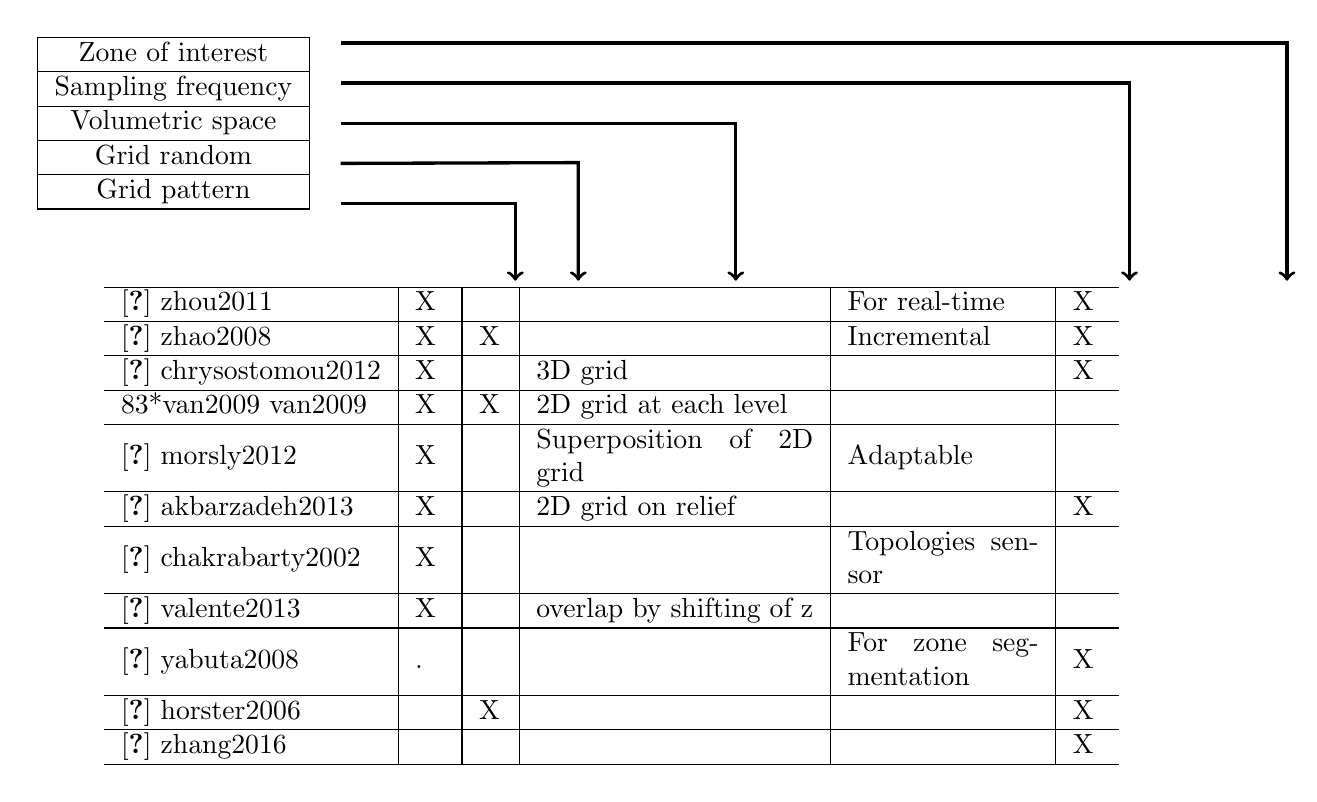
\begin{tikzpicture}[right]
\node (a) at (0,0)
{

\begin{tabular}{|c|}
\hline
   Zone of  interest \\ \hline
   Sampling frequency   \\\hline %\vdots
   Volumetric space  \\\hline
   Grid random \\ \hline
   Grid pattern  \\ \hline
\end{tabular}
};

\node[yshift=-3.89cm,xshift=-1cm] (b) at (a.south) 
{
\begin{tabular}{l | m{0.031\linewidth} | m{0.024\linewidth} | m{0.29\linewidth} | m{0.2\linewidth} | m{0.031\linewidth} }
\hline
%zhou2011 \citep{8*zhou2011} & $x_1$ & $x_2$ & $x_3$ & $x_4$ & $h(x)$ \\ \hline
%zhao2008 \citep{22*zhao2008} & 1 & 0 & 1 & 1 & 13.25 \\\hline

\cite{8*zhou2011} zhou2011  		&	 X	 &	     & 	   						  & For real-time    & X \tabularnewline   \hline 	
	 \cite{22*zhao2008} zhao2008 		&	 X	 &	 X   & 	   						  & Incremental	 	 & X \tabularnewline \hline     
	 \cite{82*chrysostomou2012} chrysostomou2012 &	 X	 &	     &	3D grid					  &  				 & X \tabularnewline \hline
       \citep{83*van2009} van2009 		&	 X	 &	 X   & 	2D grid at each level  	  &  				 &	\tabularnewline \hline
    \cite{87*morsly2012} morsly2012	 	&	 X	 &	     &  Superposition of 2D grid  &  	Adaptable	 &	\tabularnewline \hline
\cite{141*akbarzadeh2013} akbarzadeh2013       &	 X	 &	     & 	2D grid on relief 		  &  		 		 & X \tabularnewline \hline
   \cite{150*chakrabarty2002} chakrabarty2002   &	 X	 &	     & 	  	 					  & Topologies sensor&	\tabularnewline \hline
     \cite{164*valente2013} valente2013
     &	 X	 	&	     &overlap by shifting of z  &  				 &	\tabularnewline \hline
      \cite{170*yabuta2008} yabuta2008     &	 .	 & 	     &		  					  &For zone 
     															segmentation 	 & X \tabularnewline \hline
      \cite{171*horster2006}  horster2006  &	  	 &	 X   & 	  	 					  &  		 	 	 & X \tabularnewline \hline
      \cite{174*zhang2016}  zhang2016  &	  	 	&	     & 	 	 					  & 				 & X \tabularnewline \hline
%\vdots &  &  &  &  &  \\
%N &  &  &  &  &  \\ \hline
\end{tabular}
};
%\draw[->,ultra thick](a)--(b);
\draw [->,very thick] (3.98,1.02) -- (16,1.02) -- (16,-2);
\draw [->,very thick] (3.98,0.51) -- (14,0.51) -- (14,-2);
\draw [->,very thick] (3.98,0.0) -- (9,0.) -- (9,-2);
\draw [->,very thick] (3.98,-0.51) -- (7,-0.5) -- (7,-2);
\draw [->,very thick] (3.98,-1.02) -- (6.2,-1.02) -- (6.2,-2);

%\draw [->,very thick] (-1,0) -- (1,0) -- (1,-2);
%\draw [->,very thick] (-1,-0.5) -- (0,-0.5) -- (0,-2);
\end{tikzpicture}
 \caption{sum-up of the grid map.}
\end{table}	
 
 
\subsection{Our approach}
 Base on the different design the one finally adopted is a grid $G$ as in Eq \ref{eq:Grid} with an uniform repartition following the 2D grid pattern. The frequency adopted is fixed depending than the size of the area, the precision required and the cameras property. The frequency adopted for the following part as to be considered as dense (high sampling frequency).
  The grid is placed on the floor of the area to control. Floor is always considered as flat without relief. The zone of interest can vary depending on the need of the experimentation, but the design chosen is flexible to apply if necessary the formulation form the Eq:\ref{eq:PcFull} with mostly $k=1$ and $p=1$, also a set $U$ is used to represent the non-interesting zone as it was presented in eq \ref{eq:setU}.

%%%%%%%%%%%%%%%%%%%%%%%%%%%%%%%%%%%%%%%%%%%%%%%%%%%%%%%%%%%%%%%%%%%%%%%%%%%%%%%%%%%%%%%%%%%%%%%%%%%%%%%%
%%%%%%%%%%%%%%%%%%%%%%%%%%%%%%%%%%%%%%%%%%%%%%%%%%%%%%%%%%%%%%%%%%%%%%%%%%%%%%%%%%%%%%%%%%%%%%%%%%%%%%%%
%%%%%%%%%%%%%%%%%%%%%%%%%%%%%%%%%%%%%%%%%%%%%%%%%%%%%%%%%%%%%%%%%%%%%%%%%%%%%%%%%%%%%%%%%%%%%%%%%%%%%%%%
\section{ Cameras coverage}\label{sec:CamerasCoverage}


Once the area to cover is described by the grid, the next step is to verify for each point of the grid if one or more cameras cover it, based on Eq: \ref{eq:PciK} with $k=1$.\\
To verify if each points of the grid is covered by a camera. It is primordial to talk about what is a camera, what kind of camera are appropriate and their projection model. 

%%%%%%%%%%%%%%%%%%%%%%%%%%%%%%%%%%%%%%%%%%%%%%%%%%%%
\subsection{ Cameras definition}\label{sec:CamerasDefinition}

The closest projection model to the human view is the perspective projection. The perspective projection is also the more common and more especially in the field of area coverage as in example \cite{101*topcuoglu2009,33*reddy2012,8*zhou2011,82*chrysostomou2012,22*zhao2008}. Other model of cameras or vision sensor can be used as for example omnidirectional with a $360^{\circ}$ of field of view as \citep{43*erdem2006,150*chakrabarty2002,174*zhang2016}. 
Here we are only focussing  on the camera perspective due to its wide use.  \\

The pin hole or in Latin the "camera obscura" (see Figure\ref{fig:cameraObscura}) is at the origin of the geometry model for the perspective projection.\\
\begin{figure}[t!]
\begin{center}
 \minipage{0.65\textwidth}
   \includegraphics[width=\linewidth]{img/PinholeCam.png}
  \caption{ Pin hole camera model.}\label{fig:cameraObscura}
  \endminipage\hfill
\end{center}
\end{figure} 
 The pin hole model is commonly composed by box (or chamber) hermetically closed to light, excepted by a small pin hole on the middle of the front side. All the ray of light reflected by the object of the world and passing by the small hole are projected onto the back side of the box. Each ray of light passing by the hole is  projected on the plan (inside the box). This plan became the reversed image of the world and can be recorded by a film or a digital sensor. 
 Due to the simplicity of the pin hole model, the calibration and camera projection estimation is simplified.\\
%  Based on it, the camera projection is dependent then few parameters intrinsic (as focal length, sensor size,...) and extrinsic (as the position $x,y,z$ and orientation $\alpha,\beta,\gamma$). 
  
 
\begin{figure}[t!]
\begin{center}
\minipage{0.65\textwidth}
   \includegraphics[width=\linewidth]{img/PanTiltRoll.png}
  \caption{The rotation composed by 3 degrees of freedom on pan tilt roll$(\alpha,\beta,\gamma)$.}\label{fig:PanTiltRoll}
  \endminipage\hfill
  \end{center}
\end{figure}

%In fact the useful elements to define the projection of a camera perspective, can be stated as a set of parameters composed by:\\
\begin{itemize}
\item Three degrees of freedom of the sensor’s position: $(x, y, z)$;
\item Three degrees of freedom of the sensor’s orientation: with the  the rotation in pan, tilt, and swing angles: $(\alpha,\beta, \gamma)$ 
\item Optical parameters including: the focal length $f$ of the lens, the sensor size $Sw\times Sh$, $u_{0}$ and $v_0 $  which would be ideally in the centre of the image. $\sigma_{uv}$ represents the skew coefficient between the $x$ and the $y$ axis.
\end{itemize}
%$s$ is composed by two elements $Sw$ and $Sh$ for the size of width and height (also called  the scale factor).\\

Among the parameters of the camera, only  some of them are useful to estimate the projection. They can be formalized as a vector:
\begin{equation}\label{eq:v}
v=(x,y,z,\alpha ,\beta,\gamma,f,Sw\times Sh,u_0,v_0,\sigma_{uv})
\end{equation}

Each element of the vector $v$ are used to compute the camera projection on the discretized floor. 
\iffalse 
To model the set of the cameras using the precedent notation, a set $V$ composed by $N$ cameras defined by $v$ noted:
\begin{equation}\label{eq:V}
\begin{split}
V= \{v_i\} \mbox{  , } \forall i=[1;N] \mbox{ , } N\in \mathbb{N}^*
\\
\mbox{ and } v_i= (x_i,y_i,z_i,\alpha_i ,\beta_i,\gamma_i,f_i,s_i,{u_0}_i,{v_0}_i,{\sigma_{uv}}_i)
\end{split}
\end{equation}
\noindent Where $N$ is the given number of cameras in the solution. Which is also the number of cameras in the set $V$. \\
Therefore, $V$ represent a camera networks and also a initial set of parameter for a set of cameras. $V$ can contain all the possibility, included the non-acceptable answer. A non acceptable  answer will be an answer with  doe's not respect the constraint of the problem.   
 \\ !!!!!!\\

%%%%%%%%%%%%%%%%%%%%%%%%%%%%%%%%%%%%%%%%%%%%%%%%%%%%  
  
 
    
The hole in the box is called the projection center. It is the point were each ray of light are crossing together.  \\
Based on this model, a 3D point $^CP=(^Cx,^Cy,^Cz,1)^T$ defined in the pin hole reference noted $ ^C\Re$ can be convert in to a 2D point  $^rp=(^ru,^rv,1)^T$ in the sensor reference (back side of the box) by using  the perspective projection model $pr() $: 
\begin{equation}
^rp=(^ru,^rv)= pr(^CP) \mbox{ with } \begin{cases} u= f.\frac{^Cx}{^Cz} \\  v= f.\frac{^Cy}{^Cz} 
\end{cases} 
\end{equation}
Where $f$ is the focal length (distance between the projection center and the photosensitive sensor )
the point $^rp$ is the projected point $^CP$ on the sensor. The sensor is composed by $sw$ pixel of width and $sh$  pixel of  heigh. To convert the coordinate $^rp$ of p in the pixel  that mean in the image reference $^i\Re$ : 
\begin{equation}
^ip=K. ^rp
\end{equation}
where $^ip$  is the point $p$ in the image reference composed by $(u,v) \in ^i\Re$ with $u$ and $v$ are  pixel coordinate. 


%Where $u_0$ and $v_0$ are the coordinate  of  the principal point of the image ( projection of the optic centre on to the image plan).  
%$k_u$ and $k_v$  are the magnification factors of the image on width and heigh. 

% resource http://ksimek.github.io/2013/08/13/intrinsic/
%https://jeux.developpez.com/tutoriels/OpenGL-ogldev/tutoriel-12-projection-perspective/
The cameras is called calibrated when the intrinsic parameters ($K$)are defined.  
 The intrinsic matrix $K$ is parametrized by Hartley and Zisserman and it is composed permit to represent the properties of the camera. To design the intrinsic matrix $K$ some part of the pin hole camera have to be defined :\\
  \begin{itemize}
  
 	\item $f$ is  the focal length. The focal length is the distance between the pinhole and the sensor (a.k.a. image plane)
  	\item $k_u et k_v$ are the magnification factors of the image on width and heigh ; related to the image sensor format%  les facteurs  aggrandisement de l'image 
  	\item $u_0 v_0$  are the coordinate  of  the principal point of the image ( projection of the centre optic on to the image plan)  %the les coordonnées de la projection du centre optique de la caméra sur le plan image 
  	%\item $s_uv$ qui traduit la non-orthogonalité potentielle des lignes et des colonnes de cellules électroniques photosensibles qui composent le capteur de la caméra. La plupart du temps, ce paramètre est négligé et prend donc une valeur nulle.\\
  	  \end{itemize}
		Once these elements are known the matrix $K$ can be designed :
	\begin{equation}
		K=
		\begin{pmatrix}
			k_u 	& 0 	& u_0 \\
			0 		& k_v	& u_1\\
			0 		&	0	& 1
		\end{pmatrix} .
		\begin{pmatrix}
			f 		& 0 	& 0  \\
			0 		& f		& 0  \\
			0 		&	0	& 1  
		\end{pmatrix} 
	\label{eq:K}
	\end{equation}
Finally, in order to estimate the positions of a 3D point in the pin hole camera reference $^C\Re$ in to the image reference $^i\Re$ 
$$
^ip=K.pr(^CP)
$$ 	  
 Parameter extrinsic (definition global) \\
  \begin{itemize}
 	\item$R_3x3$ = la matrice de rotation permettant de passer du repère lié à l'espace de travail au repère lié à la caméra\\
 	\item$t_x t_y t_z$ = les composantes du vecteur de translation permettant de passer du repère lié à l'espace de travail au repère lié à la caméra.\\
  \end{itemize}
 %Parameter utile pour notre cas de figure \\     fig : \ref{eq:V}\\
 
!!!!! the previous section can be largely (keep the basic introduction remove to be replace by ... !!!!!
\fi
%%%%%%%%%%%%%%%%%%%%%%%%%%%%%%%%%%%%%%%%%%%%%%%%%%%%%%%%%%%%%%%%%%%%%%%%%%%%%
\subsubsection{Coverage estimation in the literature}

%To estimate the coverage of a set of camera $V$  the cameras projection of each $v_i$ has to be computed individually.
 In order to compute the camera projection onto a grid the pin hole model is used with the parameters of the vector $v$.\\
The detail to estimate the camera projection on to the floor, based on the pin hole model and the parameters ($v$), has been detailed numerous times as in \cite{193*fu2014,181*wang2017,165*jiang2010}. In \cite{193*fu2014,181*wang2017,165*jiang2010} the camera projection is used to estimate if a point is visible by a camera, for each point of the grid. These articles handles the classic camera projection (with the 6DoF in \citep{193*fu2014} and 5DoF in \citep{181*wang2017}), both are used to estimate the 2D projection of the camera onto the floor. \\
In  \citep{193*fu2014}, the camera projection has been computed for several rotations for all the DoF. In this case, the projection can have numerous shapes (mostly parallelogram shape).
In \citep{181*wang2017}, the model of camera projection begins to be simplified by assuming some fixed parameters. The fix parameters allow more efficient by economizing part of projection computation of the camera at each time.  \\
In \citep{165*jiang2010}, the model of camera projection is used to compute one time for a fix pan and roll in order to have a coverage estimation use in a 2D map. The camera projection is finally simplified by using a kind of triangle shape.\\
 Some of them as \citep{165*jiang2010,181*wang2017,141*akbarzadeh2013} include the object occlusion. To detected the part of the area occluded by an object, the solution commonly proposed (as is well explain in  \citep{181*wang2017}) is to check the line made between a point covered ($g_i \in Pc$) and his camera. If this line is intersected by at least one object in the scene, the point $g_i$ cannot be considered any-more as covered. 
%  Despite the simplicity of the computation numerous operation have to be done to compute the camera projection onto the floor. \\

To go further other model and formulation inspired by the pin hole model has been proposed as \cite{87*morsly2012,141*akbarzadeh2013,146*li2011,194*fu2010}. These models are inherited for the camera projection and adapted to fit their problems. \\
In \cite{87*morsly2012,194*fu2010} the camera is considered to be placed on the floor with a fix pan (with the looking direction almost parallel to the floor). Therefore the camera projection is simplified by an isosceles triangle where the shape depends on the focal length.\\
In \citep{141*akbarzadeh2013} the camera projection is also simplified in order to have a kind of isosceles triangle shape with considering the depth of view of the camera.\\
In \citep{146*li2011} thanks to a fix pan and focal length, the camera projection is simplified in order to have a rectangle projection onto the ground. The sweep is designed consequently to the size of the camera projection, in order to minimize the overlap and have full coverage of the area.  


One of the common point of the method present in \cite{87*morsly2012,141*akbarzadeh2013,146*li2011,194*fu2010,22*zhao2008,33*reddy2012,193*fu2014,181*wang2017,165*jiang2010}   is the computation of a camera projection on to a grid. The computations necessary to estimate, if a point of the area is cover are not considered as really greedy (in time). But have to be done to each point $g_j$ of the grid and for each camera $v_i$ of the network.
	\begin{equation} \label{eq:sum sum v g}
		\sum_{j=1}^{m}\sum_{i=1}^{n}f( v_i,g_j)
	\end{equation}
Where $n$ the number of cameras in the network; $m$ the number of point in the grid; \\
This equation (Equation \ref{eq:sum sum v g}) does not take in account the occlusion by few obstacle $Obj$. If we add the potential occlusion by $k$ object: 
	\begin{equation}
		 \sum_{k=1}^{k}\sum_{j=1}^{m}\sum_{i=1}^{n}f( v_i,g_j,Obj_k)
	\end{equation} 
 
The function $f(...)$ in charge to compute a camera projection will be called in the worst case for each camera, in order to evaluate the complete coverage of the area. This numerous call will greatly increase the time computation of the coverage. It is even worst when numerous cameras projection ($n$) has to be computed at each turn of a long optimisation process.\\
In this condition the efficiency of the function $f()$ in charge then, computes the coverage estimation is primordial, due to the numerous call.



\subsubsection{Coverage estimation optimization} \label{sec:coverageEstimation}
Design an efficient cost function is necessary to reduce the time computation and estimates the area covered. A good estimation of the area covered is primordial for the optimisation process. 
  The computation of a camera projection have to be minimized with some basic assumption depending on the problems.\\
Considering our case, where a camera is fixed on a UAV with a looking direction orthogonal to the ground, without any rotations in $\alpha$ (pan) and $\beta$ (tilt). It is possible to compute for a given altitude the area covered by one camera, based on the given parameters. Especially the focal length $f$, the altitude of the cameras and the sensor size $Sw\times Sh$. 
In this model the camera projection is always a rectangle as described in Figure \ref{fig:cam_proj}. To estimate the shape of the rectangle with is deduced from the ratio of $s$ and the size of this rectangle with is deduced from $(f ,s ,A)$. Where $A$ is the altitude. The altitude is the distance between the grid and the cameras, in the simple case $A$ is considered to be equal to $z$, when the grid is on the floor.  \\
The basic computation to estimate the size of a camera projection :

%\begin{equation}
%s= [Sw ; Sh]  %\mbox{   } Sw,Sh \in \mathbb{N} 
%\end{equation}
%
%\noindent Where $Sw$, sensor size width. \\
%Where $Sh$, sensor size height.
	\begin{equation} \label{eq:etaUpsilon}
 	 \begin{split}
		\eta = 2\times \tan^{-1} (\frac{Sw}{(2\times f)}  ) 
 	   \\
		\upsilon = (\frac{Sw}{Sh} )\times \eta
 	 \end{split}
	\end{equation}
Where $\eta$, $\upsilon$ are the horizontal and vertical camera fields of view.\\
Estimating the width and height of the rectangle projected on the ground depend on the altitude $A$ :
	\begin{equation}\label{eq:WrHr1}
		\begin{split}
    		Wr= 2\times A\times\tan \eta
    	    \\
    	    Hr= 2\times A\times\tan \upsilon
    	 \end{split}
	\end{equation} 
	\begin{figure*}[t!]
		\centering
		\minipage{0.85\textwidth}
  		\includegraphics[width=\linewidth]{img/CamProject1Bis.png}
  
 	 	\endminipage\hfill\caption{Camera projection onto a grid. The grid is placed on the floor to discretize 	the area covered.}\label{fig:cam_proj}
	\end{figure*}

Therefore, the size of the rectangle projected onto the floor is $(Wr,Hr)$ for the width and height. The values of $Wr$ and $Hr$ are directly linked to the altitude of the camera. In the simple case and in the initialization, $A$ is equal to $z$  and $z$ is selected in a range given by the UAV or the user. \\
Once the couple $(Wr,Hr)$ as been computed for a $A=z$ it is easier to change the altitude of the camera. The rectangle projection will be affected in proportion.
	\begin{equation}\label{eq:A.coef}
		\begin{split}
 		   	f(A)= (Wr,Hr) \text{ based on eq \ref{eq:WrHr1}}\\
    		f(A.Coef)=f(z)= (Wr.Coef,Hr.Coef)      
    	 \end{split} 
	\end{equation}
Therefore, to any altitude $z$ is existing $A.Coef$ where the size of the camera projection onto the floor is $(Wr.coef, Hr.coef)$. Thanks to this the eq: \ref{eq:etaUpsilon} and eq: \ref{eq:WrHr1} have to be compute once  for a given focal length $f$ and sensor $s$ with an simple $A=z$. Adding simple $Coef$ the size of camera projection can be easily simplified in order to limit the useless computation (only 2 multiplication instead then equation \ref{fig:cam_proj} and \ref{eq:etaUpsilon}.
The model of camera projection is greatly simplified by the UAV assumption (fix pan, tilt and focal length). That permits to consider the camera projection as a simple rectangle with a size directly related to the altitude (by using a simple coefficient $Coef$).\\
%The simplification by modelling all the cameras with a fix orientation and same ability (in order to have a rectangle projection onto the ground) 
All this simplification helps the cost function to be fast and efficient. \\

\subsection{Parameter to optimize }\label{sec:parameterToOptimize}
% en raison de 
By dint of the simplification presented previously the vector of parameters (\ref{eq:v}) can be simplified too.\\
To summarize,  the computation of one camera projection onto the floor, where the floor is represented by a grid for the area to cover, and the camera is in altitude with a looking direction orthogonal to the floor. Just few parameter are necessary  as showed in equation  \ref{eq:etaUpsilon} %{eq:WrHr1 , }
to \ref{eq:A.coef}. Thanks to that the equation (\ref{eq:v}) can be reduced with keeping only the position of the camera and the roll as:
	\begin{equation}\label{eq:v2}
		v=(x,y,z,\gamma )
	\end{equation}
	or also
	\begin{equation}\label{eq:v2}
		v=(x,y,A.coef,\gamma )
	\end{equation}

Reducing the number of  parameters, passing to the equation \ref{eq:v} to \ref{eq:v2} are really usefully to the optimisation of the problem. The reduction of the number of parameter will greatly affect the optimisation process.\\
 Indeed, in addition to reduce the time computation, this simplification reduce the number of parameters to optimize.   

Until now the camera projection estimation as was addressed with only one camera. But we want to compute the coverage for a set of cameras. \\
The solution is based on the previous estimation for the camera projection, but adapts to the location of each camera. By  positioning the rectangle projection to have the center of it at the $x$ and $y$ position and compute the occupation grid.\\

In order to win a bit of time, each point of the grid already cover by a camera are note tested for the next cameras. This small modification will impact positively the computation time for the coverage estimation of a network of camera. That mean in the equation \ref{eq:sum sum v g} the value of $m$ decrease as $i$ increase. More exactly  the size of $m$ decrease as  the area coverage increase.  
\\

\subparagraph{Representation of the parameters to optimize. \\}

Until now, the camera formulation is adapted to one camera, to represent the problem we need a set of cameras. The precedent notation can be extended to have a set of $V$ composed by $n$ cameras defined by the parameters of $v$:

	\begin{equation}\label{eq:V}
		\begin{split}
			V= \{v_i\} \mbox{  , } \forall i=[1;n] \mbox{ , } n\in \mathbb{N}^*
				\\
			\mbox{ and } v_i= (x_i,y_i,z_i,\gamma_i)
		\end{split}
	\end{equation}
\noindent Where $n$ is the given number of cameras in the network. The coordinate of a camera $v_i$ with are the $i$th camera of the network is defined  with $x_i, y_i, z_i,$ for a given room and $\gamma_i$ the roll rotation (portrait or landscape). The parameters not contained in $V$ and used to compute the cameras projection are  identical for all the set $V$, and are fixed at the beginning of the optimization.\\
Therefore, $V$ represents a solution. $V$ contain all individual positions and orientations of the set of cameras for a predefined focal length, sensor size and map depending on the problem.% wish also include the potential constraint as  some restriction on the map.\\
Obviously all the solution $V$ are not a "possible solution" for our problem. Some solution $V$ does not respect the set of constraint noted $E$.

So that the $V$ should respect the constraints of the set $E$ (see Eq.\ref{eq:Vs}). Among the constraint few of them was already disused, as the occlusion, the map restriction, the k-coverage, or some constraint more specific to the problems (as saw in chapter \ref{chap:stateOfTheArt}).\\
 The "possible solution" $Vs$ must take in consideration with the set $E$ as :

\begin{equation}\label{eq:Vs}
Vs=V \mbox{ , iff } E(V)=\begin{cases}1, & \mbox{  iff } E_i(V)=1 \mbox{ , with } i=1...Nc \\ 0, & \mbox{otherwise} 
\end{cases} 
\end{equation}
Where $E_i(V)$ is the function applied to verify  the $i$th constrains of the set $E$ on the solution $V$. $Nc$ is the number of constraints needs to be satisfied to have an acceptable solution.
That mean among all the possibles combination of parameters $V$ only the one intersect the set of the constraint $E$ are an possible solution.  If we are considering  all the $V$ and all the $E$ as two subset $Vs$ is defined as $Vs=V\subset E$. 

The problem of monitoring an area and more specifically the problem of area coverage may contain many constraints depending of the environment and the context. As example: the room shape, minimizing  the altitude,  have the best resolution, orientation of the camera, the possible occlusion,... All this constraints are included in the set $E$. 
The constraint have to be defined depending on the problems and the goal.
\section{Cost Function}
\subsection{Constraint}\label{sec:constraint}

Make the exhaustive list of all the constraints for the problem of cameras positioning is not really interesting and almost impossible. The constraint can be numerous and depend mainly of the problem formulation and the context. Like that few of them was briefly introduced in the previous section as in chapter \ref{chap:stateOfTheArt}, section \ref{sec:coverageEstimation},... This part is focus on the list of the constraint used in our case and detail their design.

The constraint considered in this work are : 
\begin{itemize}
	\item Fix number of the cameras.
	\item Fix parameters of the camera.
	\item No rotation  on  $\alpha$ and $\beta$ (pan and tilt).
	\item Possible fix altitude.
	\item Altitude boundary (not too hight, not too low).  	
	\item The map boundary (rigid rectangle).  
	\item Non rectangles map with possible holes.
	\item To have some fix cameras in the set. 
	\item The resolution.\\

\end{itemize} 
\subparagraph{Fixes number of the cameras}
One of the first constraint is the fix number of cameras. This constraint as some others (detailed latter) are  useful to simplify and restrict the possibility of the problem. This constraint permits us to focus on the fine optimisation (as in \citep{22*zhao2008} where both are tested). The number of cameras is fixed at the beginning of the optimisation and no more camera will be added during the optimization process.  

\subparagraph{Fixes parameters of camera and no rotations}
Fixes parameters of the cameras and no rotations ($\alpha$ and $\beta$) has been introduced previously (section \ref{sec:parameterToOptimize}). These constraints imposed by the use of an UAV are also an advantage for the optimization by simplifying the coverage estimation and limit the number of parameters to optimize. The parameters are fixed at each beginning of the optimization.

\subparagraph{Fixes altitude}
 The fix altitude is a constraint use in order to limit the number of parameters to optimize. The use of this constraint is used to reduce the complexity (see section \ref{sec:OptimizationComplexity}). It is also useful for other assumptions, as a camera on the celling or for a submarine  \cite{66*galceran2013}. This constraint is an optional constraint and is not commonly used in the experiment presented in the following section.   

\subparagraph{The altitude boundary}\label{sec:altitudeBoundary}
 When the altitude is not fixed some limit must be chosen to avoid the extremely high and low altitude. The highest altitude will be fixed depending on the UAV ability and other restrictions as the laws. The lowest altitude has to be fixed for the safety of the user under the UAV.  
In practice the boundary of the $z$ is defined with :
 \begin{equation}\label{eq:boundaryZ}
   \inf z\leq A.Coef\leq \sup z  
 \end{equation} 
 Where $\sup z$ is the maximal altitude of the camera and $\inf z$ the minimum altitude. $A$ is the fix altitude  of a camera where the camera projection has been computed with $A=z$ with only $coef$ vary as introduced in Equation \ref{eq:A.coef}. 
 
 \subparagraph{The map boundary}
The map boundary is a constraint similar then the altitude boundary. Despite the shape of an area to cover some maximum boundary can be made. In fact for any shape as complex as it, it is  possible to encapsulate in a rectangle. The rectangle map boundary is defined by a width $W$ and height $H$. The boundary on $x$ and $y$ are:
 \begin{equation}
  \begin{array}{lcl}
  	0\leq x\leq W \\
  	 0\leq y\leq H 
  \end{array} 
 \end{equation}  
 
By associating the altitude boundary (from Eq\ref{eq:boundaryZ}), a cube boundary limits the position of the cameras in the 3 dimensional spaces. 
\begin{equation}\label{eq:3dBoundary}
  \begin{array}{lclcl}
  	0\leq x\leq W \\ 0\leq y\leq H  \\ \inf z\leq A.Coef\leq \sup z  
  \end{array} 
 \end{equation} 
 
 \subparagraph{Non rectangle map with possible hole.} \label{subPara:MapConstraintAndObstacle}
Despite the rectangle boundary of the area, the map to cover can be much more complex than a simple rectangle and can take any kind of shape. Also the shape of the area can be composed by holes. The figure \ref{fig:boundaryMap} illustrate the map complexity. The black part of the map are the zone with are out. That mean these sub-parts have not interest to be covered.
 \begin{figure}[t!]
 \begin{center}
\minipage{0.85\textwidth}
   \includegraphics[width=\linewidth]{img/BoundaryMap2.png}
  \caption{Map to cover with the map boundary in red (W and H size) in black the sub-part have no interest to  be covered.   }\label{fig:boundaryMap}
  \endminipage\hfill
  \end{center}
\end{figure}
To take in account this constraint the gird has been designed with removing some of this points.
The grid $G$ is reduced in order to have only the points in the white sub-part. In this example each white pixel of the map is points of the grid. 
Concretely this implementation is easier for the complex map and has also some advantage. \\
Among the advantage, the flexibility of the grid customization. That allows the optimization to try some exotic solutions, as allowing the camera  position on the black sub-part or in a border of it during the optimization.  Obviously the exotic solution with a cameras position on the black side does not increase the coverage rate  but if the optimisation converge correctly no camera will be on the the black sub-part of the map (or small part of it).

\subparagraph{Some fix cameras in the set}
Having some fix cameras position in the set of cameras, is an optional constraint. This allows to have few manual cameras position from an user or other algorithms.
One case can be to have some specific area as the entrance where have to be surveyed by a cameras dedicated to.  
To implement this constraint the solution applied during the experiments (presented later) is to adapt the map by removing the point of the grid $G$ cover by the sub-set of fix cameras (as if these points of the grid was covered).

\subparagraph{The resolution}
The resolution of the images is related then the sensor size (in px) and the distance between the camera and the object filmed. In our case, the sensor size is fixed by the properties of the camera mounted on the UAV and the object filmed is the floor of the area to cover. In this case, the distance between the camera and floor is the altitude. \\
The resolution constraint has to maximize the resolution. In order to maximize the resolution during the optimization the altitude criteria is modified in order to be the lower possible.\\
Considering only the resolution constraint as minimizing the average altitude of the cameras is harmful for the coverage optimization.
Consequently, during the optimization a trade off between the altitude (and the related resolution) and the coverage rate have to be done $\min{\frac{\sum^n_{i=1}{A.coef_i}}{n}}$ and the coverage rate. In order to manage this trade off, the average altitude of the cameras is included in the cost function (see section  \ref{sec:costFun}).  
 
\subsubsection{Constraints types}
 
Among the constraints listed different priorities and restrictions exist. Indeed the constraint can be considered in 2 sub-class. 

\subparagraph{Hard Constraint}
 Some of the constraints presented are called "Hard constraint". \\
 The hard constraints limit the possible solution by do not allowing the solution with does not respect it. This hard constraint is directly used during in the optimisation process to prohibit any solution to be out of this boundary. This hard constraint has to be integrate in the optimization process in order to cannot generate a solution with does not respect it. Consequently the hard constraint can some times slow down the generation of the individuals.\\ 
 For example, the 3D boundary as defined in Equation \ref{eq:3dBoundary} is a hard constraint. Each cameras position must be inside the 3D boundary.\\
 
 \subparagraph{Soft Constraint}
 In the other case, some constraint can be considered as "Soft Constraint".\\ 
 The soft constraints has to minimize the set of error. If a soft constraint is not fully respected the solution can be considered as acceptable and this small amount of error does not affect so much the final answer. In this case the soft constraint is assimilate to small acceptable error. \\
 The soft constraint leaves the possibility during the optimization to do some mistake in order to learn about it.  
 If the soft constraint is noted $\epsilon$ and the hard constraint are noted $ \varepsilon '$ like that the constraint set is $E=\epsilon+\varepsilon'$.\\
 
% \begin{equation}
% 	\max f(Vs) -\epsilon  \mbox{  } \forall Vs \subset \varepsilon'
% \end{equation}
  \begin{equation}\label{eq:constraintEpsilon}
 	\max f(Vs) - \min \epsilon  \mbox{  } \forall Vs \subset \varepsilon'
 \end{equation}
 
The objective is to maximize the coverage of a set of cameras ($f(Vs)$) with respect the hard constraints $\varepsilon'$ and minimized the error form the soft constraints $\epsilon$.
Concretely the soft constraints are commonly integrated in the Cost Function as can be the resolution or the fix number of the cameras by the grid design. 


\subsection{The cost function implementation} \label{sec:costFun}

The cost function has the mission to estimate the quality of an answer. In our case, an answer is the position  of a set of cameras. The cost function is essential in the process of optimization as that was introduced in the section \ref{sec:CostFunctionGA}.

The cost function has to estimate the area cover by a set of cameras in order to do that the area is discretized by a grid as in section \ref{sec:Grid}. \\
The grid customization permit to introduce some of the soft constraint as the complex shape of the map by removing the point out of the area to cover. Also the fix cameras are added in the grid points as already cover area. \\
The grid modification will allow the cameras position to cover the area already covered and removed form the grid. The consequence of it will be to reduce the coverage rate possibility. The optimization will have to minimized this error.

To evaluate the coverage of a set of cameras is essential to can estimate the cameras projection of each, as detailed in the section \ref{sec:CamerasDefinition}. The area cover by the $j$-Th camera is noted as in equation \ref{eq:PciK} (where $Pc\in G$). By iteratively repeated this for each camera of the set the full area coverage is computed (as equation\ref{eq:sum sum v g}). 

Based on, the  simplest cost function is the coverage estimation.
\begin{equation}\label{eq:CostFBase}
C(Vs) =  \frac{\sum_{i=1}^N{Pc_i} }{m}   
\end{equation}
Where $N$ is the number of cameras; 
$m$ represent the number of points needed to describe the grid $G$ (as in Equation \ref{eq:Grid}); $Vs$ is the solution with respect the hard constraint.
The cost function $C(Vs)$ give the quality of the solution $Vs$.

This version of the cost function $C(Vs)$ does not take in account the resolution constraint. The resolution is  strongly linked with the camera altitude $z$ (as show in \ref{sec:altitudeBoundary}).
 A criteria must be added in the cost function formula of the Equation \ref{eq:CostFBase}. The average of the altitude $z$ is used and have to be included in the cost function.
 \begin{equation}\label{eq:CostFResolutionPart1}
\overline{z}= \frac{\sum_{i=1}^N z_i}{N}     
\end{equation}

 If the resolution is strongly related then the altitude the average of it ($\overline{z}$) can be considered as a part of the soft constraint ($\epsilon$)  in the equation \ref{eq:constraintEpsilon} and the equation \ref{eq:CostFBase} may be updated as : 
 
 \begin{equation}\label{eq:CostFResBase}
C =  \frac{\sum_{i=1}^N {Pc_i}}{m}  - \frac{\sum_{i=1}^N z}{N}     
\end{equation}
 
The equation \ref{eq:CostFResBase} is used in the cost function to add the resolution constraint. The consequence of it, is the optimization will try to minimize the average altitude and maximize the coverage with no priority. Concretely by just applying this equation  \ref{eq:CostFResBase} the optimization will first minimize the average altitude by positioning all the cameras at the minimum altitude (with respect the hard constraint of altitude boundary) and in second time try to maximize the position (on $x$ and $y$) of the cameras. 

In order to have a priority  between the coverage and the altitude a weigh has to be made on the equation \ref{eq:CostFResBase}. The weigh have to be chosen carefully.
The weight has to be auto-adaptable depending on area covered. In order to give more priority to the coverage when the coverage rate is low and add importance to the resolution when the area is already well covered. The coverage has to stay the priority the resolution must be optimized in a second time.
The best solution to do that, is to link the weight of the resolution criteria with the coverage rate.

\begin{equation}\label{eq:CostFResPondere}
  \sigma \times \sum_{i=1}^N {Pc_i} \times \frac{\sum_{i=1}^N z}{N}     
\end{equation}
Where $\sigma$ is a weighting coefficient at 0.06 to reduce the priority on the resolution criteria. 
Based on it the final cost function is: 

\begin{equation}\label{eq:CostF}
C(Vs) =  \frac{\sum_{i=1}^N{Pc_i}  - \delta  \times \sum_{i=1}^N {Pc_i} \times \frac{\sum_{i=1}^N z}{N}  }{m}   
\end{equation}

Thanks to this formula, a proposed answer $Vs$ can be evaluated and returns the quality of the solution for the problem of the coverage maximisation and the minimization of the altitude in the second time. The cost function integrate all the soft constraint either by the design of the grid or by the formula of the cost function $C()$.

The cost function presented is the final one, but the building of it was an incremental work and numerous version was test in term of weight, priority, and constraint. The one presented here is the more equilibrated.\\ 
Despite that some of the work  presented in the following section are made with the basic cost function from the equation \ref{eq:CostFBase}. In this case, the element composing $v$ can be reduced as only $v=(x,y,\gamma)$.\\

The final and complete cost function $C(Vs)$ have as input a vector $Vs$ with are composed by all the cameras position and orientation of the network. It is also composed by the map of the area to cover $G$ where $G$ include the soft constraints as the room shape, the fix camera. The constraint of resolution is added by using the average altitude in the equation \ref{eq:CostF}.
The value is returned by the cost function $C(Vs)$ is the quality of a solution to our problems of coverage using an UAV.






%%The use of an UAV to cover an area allow the simplification of coverage computation as well as the numbers of parameters to optimize.
%% !!!!
%%Thanks to the simplification of the problem due to the used of an uav the parameters to optimize can be reduced. (as in eq: \ref{eq:v}
%%Thanks to the simplification the element to optimize for an efficient coverage can be limited to pass from Eq. (\ref{eq:v}) to  Eq.(\ref{eq:v2}) as shown: 
%%\begin{equation}\label{eq:v2}
%%v=(x,y,A,\gamma )
%%\end{equation}
 %%%%%%%%%%%%%%%%%%%%%%%%%%%%%%%%%%%%%%%%%%%%%%%%%fin de la camera pin hole explication%%%%%%%%%%%%%%%%%%%%%%%%%%%%%%%%%%%%%%%%%%%%%%%%%%%%%%%%%  
%    
%In the following part a vision sensor is employ to acquire the image of area to control. The vision sensor may be a common camera with different parameter as:
% \begin{itemize}
% \item Every camera has a position  in  $(x, y, z)$;
% \item Every camera  has an orientation composing to 3 degrees of freedom  pan$(\alpha$),  tilt$(\beta)$, roll$(\gamma)$, see Figure \ref{fig:PanTiltRoll}.
% \item Every camera have different optical parameters and the helpful to take in consideration for coverage estimation is the focal length $f$ and the sensor size $s$(based on the formulation of Chrysostomou et al[82]). 
% \end{itemize}


 
%%%%%%%%%%%%%%%%%%%%%%%%%%%%%%%%%%%%%%%%%%%%%%%%%%%%
 \section{Optimization complexity} \label{sec:OptimizationComplexity}
 
%To cover an area with a certain amount of sensor many solutions can be possible.
In spite of the simplification presented before, the problem stays complex. There exist many positions for each camera to cover an area with a certain amount of sensors. This number of position can be estimated as follows.\\   
Each camera defined by the position on $x, y, z $ and $ \gamma$ can be set anywhere in the search space named $Sp$ : 
\begin{equation}\label{eq:SearchSpace}
 Sp=(W\times H \times ( \max(A)-\min(A)) \times 2 )  Sp \in E 
\end{equation}
Where $W$ and $H$ are the size as width and height of the area to cover, $\max(A)-\min(A)$  is the range  of possible altitude. 2 is to define the roll $\gamma$, as the rectangle projection is horizontal or vertical (landscape or portrait). The search space $Sp$ allows to take in consideration some strong constraint $E$ like the boundary of the area or the restriction in the degree of freedoms.

The problem of the search space is the propensity to increase rapidly as the area grows. This phenomena is accentuated by the size of the set of cameras $N$.
%It is possible to express the size of the search space as a succession of product for estimate the number of feasible position on $x, y, z $ and $ \gamma$ for each combination of the set cameras : 
%\overset{N}{\underset{Sp}{e}
 \begin{equation} \label{eq:Combinaison}
 \begin{pmatrix} N \\ Sp \end{pmatrix}  = \frac{Sp!}{N!(Sp-N)!} = |Vs|
 \end{equation} 
 Where $|Vs|$ is the number of possible solution for a set of $N$ cameras in the worst case. %$|Vs|$ is the 
 %  \begin{equation} \label{eq:SearchSpace}  \sum_{n=1}^N \sum_{x=1}^{W} \sum_{y=1}^{H} \sum_{z=1}^{)} \sum_{\gamma=1}^{2}Pc_i  - \sum_{k=1}^{E}Pc_i=Vs  \end{equation}
 In fact the size of the search space ( as Eq. \ref{eq:SearchSpace}) associate to the set of $N$ cameras (as Eq.\ref{eq:Combinaison}) make an exponential number of possible solution depending mainly then the size of the area and the number of the cameras in the network. \\
 Obviously in view of this behaviour the use of a deterministic solution based on a heuristic does not seem to be a good answer to have an efficient solution. In addition the number of possible solutions $|Vs|$ makes the computation of an optimal almost impossible due to the numerous local minima. This kind of problem can not be used with an algorithm dedicate to the research of global optimal solution but need to be used with an algorithm focusing of optimizing the solution and returning an acceptable solution.\\
 The formulation of the problem is primordial in order to reduce the size of the search space and give a chance to the optimization to converge.




%%%%%%%%%%%%%%%%%%%%%%%%%%%%% FIN coverage estimation%%%%%%%%%%%%%%%%%%%%%%%%%%%%%%%%%


 

\chapter{Waypoints positioning } 
\minitoc
To remind, the main objective is to propose an efficient path to can cover an area using a camera mounted on an UAV. The solution proposed here, is to focus on optimizing the position of a cameras set to fully cover an area in a first time. When set of optimized cameras pose is found the position can be used as waypoints for an UAVs path. Indeed find an optimized position for each camera of a given set is primordial. The following sections are dedicated to the optimization of it. 




%\section{An optimization problem.}

During the previous sections, the problem was discussed as an optimization problem. The formulation of the problem was presented  and  the complexity of the problem was disused in the section \ref{sec:OptimizationComplexity}. Thanks to this preliminary result the following section is only focused on the optimization process. 



\section{PSO }

The PSO (Particle Swarm Optimization) is an algorithm dedicated to the optimization problems. It is an stochastic algorithms from the family of evolutionary algorithms (see  chapter \ref{chap:EA}). 
The PSO is a relatively young compared then the other EA. It was developed by Russel Eberhart and James Kennedy in 1995 [148* bis]. The concept of PSO is to optimize iteratively a continuous non linear function. To do that the PSO is inspired by the behaviour of animals. As it appends here from the bird flocking, fish schooling and swarming theory. These are animals working in a group to find food. 
The direction to take is not decided by one leader, but by all individuals of the swarm by relaying just few informations as what quantities of food their found. 
The swarm composed by numerous individuals became smarter and more efficient to reach their objective. 
The algorithm proposed by Russel Eberhart and James Kennedy in [148* bis] \cite{148*eberhart1995} are directly inspired by these behaviours.

The methodologies used, is to examine each individual or also called particles as a solution of the problems. The problem is optimized at each iteration. To do that each solution must be comparable and quantifiable. At each iteration, each particle has to be tested by a cost function in order to discriminate the best particles of the swarm. The cost function and the design of it has been detailed in the chapter \ref{chap:formulation}.
When the best particle is found at the end of an iteration, the other particles of set, try to change their initial direction to converge more or less quickly to the actual best. 
Indeed the power of this algorithm is to obtain a very basic individuals behaviour to guide the particles. 
Each particle is guided by 3 behaviours.
 \begin{itemize}
 \item  This own velocity $V_k$. 
 \item  This own best solution $P_i$.
 \item  The best solution $P_g$.
\end{itemize}  
Here the velocity represents the useful speed of the particle to converge to the best solution. More the velocity is high more the step at each iteration will be long. 
The behaviour of the particles $X_k$ are modelled by the following equation to obtain the new position $X_{k+1}$ :
\begin{equation} \label{eq:PSO}
\begin{split}
 V_{k+1}= \omega V_k +b1(P_i -X_k)+b2(P_g-X_k)
\\
\mbox{ and } \\ X_{k+1}=X_k+V_{k+1}
\end{split}
\end{equation}

Where $\omega$ is the inertia. $b1$ is random value between 0 and $\phi_p$ and $b2$ is random value between 0 and $\phi_g$. $\phi_g$ and $\phi_p$  are the scaling factor to search away from the particles is best known position (Default: 0.5). 

Thanks to this basic behaviour of the particles the swarm can coverage to a global solution. 
To have an efficient optimization just few parameters must be set-up for the PSO.  
The more important are the inertia of the particles, the size of the swarm and the initial dispersion.
\begin{itemize}
\item The inertia will globally  help the particles to keep their initial velocity. The consequences of the high value of inertia is to explore more the search space and therefore the convergence will be longer. 
\item The size of the swarm  have an impact on the convergence time (in number of iteration) and the also time computation. Indeed a big amount of particles in the swarm  means more exploration of the search space at each iteration, but also more comparison to find the best particles (the comparison may have a non negligible computation time). 
The swarm size is commonly fixed but can be as the population in the GA (see section \ref{sec:Population} ) dynamically adjusted during the optimization process. 


\item The initial dispersion of the swarm can be a decisive element as the population for the GA (see in \ref{sec:initPOP}). For the PSO the use of an heuristic to initialize all the particles of the swarm is not recommended due to this important risk to converge prematurely in a local minimum. The random dispersion appear  as the more appropriate for a global optimization. On the other hand the fast convergence and the PSO ability to climb the hill to go out of the local minima can be used in order to refine an other optimized solution. The principal risk is to optimize around the initial dispersion and  do not explore correctly the search space.  
\item Other criteria as $\phi_g$ and $\phi_i$ are minor but can be useful to   have a realy fine adjusted PSO.
\end{itemize}

Finally to summarize the PSO is efficient in term of optimization despite a very basic behaviour of each particles. Each particles have this own velocity defined part way by the random and controlled by a global parameters; the inertia.
 The power of PSO is at same time this efficiency to solve the optimization problem and this simplicity of use. In fact the PSO need at minima  few element to work properly:
 a cost function, an inertia parameters and the size of the swarm. These efficiency and simplicity of use explain this popularity during the last decade.
 





%-the initial dispersion of the particles \\
%- size swarm \\
%- stopping criteria \\
%- inconvenient 


\section{Random selection }

The random selection (named RS) is a very basic algorithm. It is used as a reference points for the comparison of different algorithms. The RS does not use a complex meta-heuristic and is perfect to compare the efficiency of the other algorithm.

The random selection works by randomly generate numerous solutions. Among the solutions randomly generated the best solution is kept as the optimized global solution. The RS allows to look through the search space by randomly try different  possible solution. The search space exploration by the RS is only made by random sampling with any optimization method. 
Indeed the RS is used as a reference points for the other algorithms. If the RS get a similar result with the same amount of the cost function call, the algorithm compared can be considered as not more efficient then a simple random solution. 
The RS is used to the search for the optimization algorithms and this appropriate parameters as the reference point and evaluate the efficiency of the chosen algorithms.


  

PSO camera position 
8 33 87 84 143(transitor) 193 194 200(capter 360)201
148 origine de PSO. 
PSO[84 8 33 143] 87 193* 194* 200* 201* 

228*(hibrid) 161* 158* 78 GA VS PSO

\section{Algorithm comparison }\label{sec:GAvsPSO} 
%
To solve the problem of cameras position (or waypoints) the possible usable algorithms are varied as that was discussed in the chapter \ref{chap:stateOfTheArt} (see the sum-up tables \ref{tab:sum-up1} and \ref{tab:sum-up2}).
Among the algorithms studied in the literature the EA family appear as the more suitable to have an appropriate answer despite the numerous constraints of our problem. The EA is a vast family of algorithms and one of the more used for our problem is the PSO (see \ref{tab:sum-up2}). The PSO give good result in many case. In the EA family the GA is one of the founders and was one of the more popular due to this great flexibility and efficiency.
 After more investigation the GA is under estimate for the problem of camera positioning unlike the PSO (see \citep{33*reddy2012,8*zhou2011,84*xu2011,143*maji2015,193*fu2014,194*fu2010}).
 Base on the work of Boeringer et al in \citep{78*boeringer2004}78*, where the PSO and the GA have been conscientiously compared. The conclusion in \citep{78*boeringer2004} is relatively open and highlights the similarity of result between two algorithms. An experimentation have to be done to find the best algorithms for the problem of cameras position in a complex environment. 



%The PSO and GA have been compared 
%The GA 
%158* 161* = GA PSO mimetic  conclusion les GA est plus long  le mimetic et  une solution intermedaire entre GA et PSO.
%78*= Comparaison entre PSO et algo génétique GA  les avantage  et les cas d’utilisation pratique.
%Papyer détatille  avec des plusier experience comparative  conclusion ouverte sur le choix mais la conlution et que le PSO offre plus de posibilité d’amélioration de par sa simplicité de mise en place et sa « récente utilisation » 

\subsection{Designe of experiment }\label{sec:DoE}
\begin{mfigures}[!]{For the experiments: (a), (b), (c) the blue rectangle represents the field of view of one camera projected onto the ground  with z=1 ($30 \times 20 $px) and (d), (e) with z=2 ($60 \times 40 $px)}{fig:Rooms_shapes} \centering
\mfigure{width=.4\linewidth}{img/fig7-a.png}{Simple room}{subfig:r1}
\hspace{1cm}
\mfigure{width=.4\linewidth}{img/fig7-b.png}{Big room}{subfig:r2}
\mfigure{width=.4\linewidth}{img/fig7-c.png}{Room U}{subfig:r3}
\hspace{1cm}
\mfigure{width=.4\linewidth}{img/fig7-d.png}{Room L}{subfig:r4}
\mfigure{width=.4\linewidth}{img/fig7-e2.png}{Big room L}{subfig:r5}
\end{mfigures}
--------to finish-----\\ (+ integration du RS)\\

To find the best coverage, many experiments have been used to compare PSO and GA. PSO is easier to implement and runs faster, but GA is more flexible and generic thanks to the many tunable parameters. 
The following subsections will provide a comparison between PSO and GA with using RS as a reference.% and give an overview of our method, which is based on GA. The comparison demonstrates the overall advantage of the latter over the former.\\
%In the literature, the PSO was often used \cite{8*zhou2011,33*reddy2012}, mostly because of the simplicity of its implementation. However, it is interesting to compare the algorithm with the GA. The two algorithms are from the same family (both are stochastic and from evolutionary algorithms).\\
To compare and evaluate their performance, we tested them in different scenarios. The scenarios have been  design to have different shape and size. The shape of the room have been design to estimate the number of cameras but due to the use of a non heuristic algorithms the shape can be considered as complex. The rooms are depicted in Figure \figref{fig:Rooms_shapes}, with areas of different size and shapes, where: 




\begin{itemize}
\item[-]    z is the height of the camera between (within the range $[1/z;z]$).
\item[-]	Figure \figref{subfig:r1} is an area of size 120$\times$80 (named Room). 
\item[-]	Figure \figref{subfig:r2} is an area of size 240$\times$160 (named Big Room).
\item[-]	Figure \figref{subfig:r3} is an area of size 120$\times$80 (named Room U).
\item[-]	Figure \figref{subfig:r4} is an area of size 120$\times$80 (named Room L).
\item[-]	Figure \figref{subfig:r5} is an area of size 240$\times$80 (named Big Room L).
\end{itemize}


The design of the experiments in Table \ref{table:table1} has been set up to identify the most efficient algorithm for the positioning of a set of cameras with maximum coverage depending on the numerous cases. 
The Design of Experiments (DOE) have been made to take in account; the  shapes, sizes, some constraint as the fix altitude and  many size of the set of cameras. The DOE has been designed to highlight the impact of the constraints on the optimization process with the GA and PSO.


\begin{table} [!htb]
\begin{tabular}{|l|l|l|l|l|l|l|l|l|l|}
  \hline
  \multicolumn{2}{|l|}{z=1 } &\multicolumn{2}{|c|}{GA}  & \multicolumn{2}{|c|}{PSO} & \multicolumn{2}{|c|}{RS}  \\  \hline
  \multicolumn{2}{|c|}{ } & GT & NC & GT & NC & GT & NC\\ \hline
  Room &  120x80 & 16 &20 & 16 & 20 & 16 & 20\\ \cline{2-8}
     &  240x160 & 64 &70 & 64 & 70 & 64 & 70 \\ \hline
  Room U &  120x80 & 12 &20 & 12 & 20 & 12 & 20\\ \hline
  \multicolumn{2}{|l|}{z=2 } &\multicolumn{2}{|c|}{GA}  & \multicolumn{2}{|c|}{PSO}& \multicolumn{2}{|c|}{RS}  \\  \hline
 Room &  120x80 & 4 &10 & 4 & 10 & 4 & 10\\ \cline{2-8}
     &  240x160 & 16 &20 & 16 & 20 & 16 & 20 \\ \hline
 Room L&  120x80 & 3 &10 & 3 & 10 & 3 & 10\\ \cline{2-8}
     &  240x160 & 15 &20 & 15 & 20 & 15 & 20 \\ \hline
  
\end{tabular}
\caption{Design of the experiment for comparing the efficiency of PSO and GA in different conditions.  (GT is Ground Truth and NW is Number of Waypoints).}\label{table:table1}

\end{table}

The Ground Truth (GT) is the minimum number of cameras required to fully cover a given area. The size of the area has been selected so that the GT can be easily estimated. 
NW is the maximum Number of cameras (or Waypoint) used for the experiments.  
At each experiment a solution is computed for a number of cameras from 1 to NW. To compare the different algorithms fairly, only 10 000 calls of the cost function are allowed for each optimization.
The optimization have been executed 8 times for each optimization process. 8 times is the minimum number of test has to be done to can have a usable average despite the hight volatility due to the randomness of the algorithms.\\ % 420*8 =3 360 test.


\subsection{ Analysis of the result }

\begin{figure}[!]
\minipage{0.99\textwidth}
  \includegraphics[width=\linewidth]{img/fig8.png}
  \caption{ Comparison of eight solutions given by the GA, with eight solutions given by PSO algorithms with a fixed altitude ($z$ equal to 1) in the big room 240x160. The ground truth for this room equals to 64.}\label{fig:bigRz1}
   \endminipage\hfill
\end{figure}
%
%
\begin{figure}[!]
\minipage{0.99\textwidth}
  \includegraphics[width=\linewidth]{img/fig9.png}
  \caption{Comparison of eight solutions given by the GA, with eight solutions given by PSO algorithms with a Z between [1/2; 2] in the room with L shape 120x80 and ground truth equal to 15.}\label{fig:RLz2}
   \endminipage\hfill
\end{figure}
After performing the several experiments (see Table \ref{table:table1}), it appears that the GA and PSO algorithms are close in performance in numerous case. Among several experiment of the DoE some particularity appear despite the globally close result of GA and PSO. Also as expected the RS is always the worst solution.
 In the following subsection  just few experiment are taken to illustrate some interesting phenomena specific to the GA and PSO for our problems.

In the case where the search space is large and numerous dimension have to be optimized the GA appear globally more efficient as in Figure \ref{fig:bigRz1}. In contrary in this case (big room with z=1) the PSO give a very bad answer close then simple RS.
%What is appearing in some case as in Figure \ref{fig:bigRz1} is the  GA is much more efficient where the search space is large (big room and big number of cameras),  as the example in Figure \ref{fig:bigRz1}. 
 Instead, PSO is more effective for optimizing small areas as in Figure \ref{fig:RLz2}. In the small room in L shape with a $z$ between 1/2 and 2, the PSO reach quickly (quicker then the 10 000 calls) to the optimal solution. Where here the optimal solution is known and equal to GT. In the same case the GA propose an optimized solution (compared then the RS) but far from the PSO.
 
 This efficiency can be explained by the small variation of the solution introduced by the PSO. However, this small variation is not enough to find an optimized solution in a big search space that occurs when many cameras are required or when the local minimum is deeper. The PSO appear really efficient in a relatively small search space where the number of dimension to optimize is not to high.
 On the other hand the variety  introduced by the GA allows the escape from local minima. This variety is helpfully  in the big search space in order to explore quickly a wide part of it. The variety introduced by the GA became an handicap for a more fine optimization. That explain the bad result obtained during the experiment is a small room. Variety of the GA negatively affect the accuracy of the solution and may require a further optimization step to refine. 
 
%-------- ajouté un exemple entre 2 forme differente qui on un resulta proche 
------------ file Grafig roomShape.txt-----\\
The DoE have been design with different shape in order to see the impact of it on the algorithms. What is appearing during the experiment is the low impact of the shape on the result of the algorithms. The experiment made in the small room (120X80) and the small room in L shape with a z between [1/2; 2](see Figure !!! and Figure !!!). The graphics (see Figure !!! and Figure !!!)  present a similar result, proof of the small impact of the shape on the algorithms.
 This small impact can be explained by the use of meta-heuristic (as PSO and GA) and not by the use of an heuristic  much more dependent of the shape (and the constraint). 
 
Thanks to that we know the two algorithms can be used for a more complex shape as that will be presented in the following experiment.

 





% Following the comparison of the 2 algorithms, the GA seems more suited for finding UAV waypoints especially if it navigates in a large room or  outdoor scenes.
%Furthermore, our comparative study demonstrates that the GA is less dependent on the shape of the area to cover. \\
%------------------
%According to the previous results, the genetic algorithm will be used during future work with no restriction at the convergence point to optimize the positioning of the waypoints in the bigger areas seen in Section  \ref{coverageOutDoor} such as in Figure \ref{subfig:satimg+mask}.\\
%---------------

%fill with the jirs 
%	\subsection{DoF Design of Experiment}
%	\subsection{Result}
%	\subsection{Explication}

\section{Hybrid GA PSO }
% ref: 76* 77* 
 

% l'hybridration peut permetre de tiré avantage des 2 algo
% \begin{itemize}
%  \item interer de l'hybridation (avantage du PSO sur l'optimisation locale et du GA) 
% \item les forme d'ibridation possible 
% \item la plus aproprier dans notre cas et pourquoi 
% \item les experience ( the experimentation  was done in the Big room in L shape as the \ref{fig:Rooms_shapes}.e)
% \item les resultats
% \end{itemize}
Thanks to the experiment done and presented in the previous section (see \ref{sec:GAvsPSO}) the GA and PSO are two algorithms efficient and complementary to solve the problem of camera positioning in the complex and potentially vast area.
  To summarize the previous comparison, it is difficult to rank the two algorithms in all the environments. GA and PSO have both advantages depending on the area and the number of cameras. GA is better in the big search space and several dimension to optimize. When PSO is efficient to refined faster the solution.
 The hybridization can be the solution to optimize the camera positions in all the condition. The aims of the hybridization is to exploit the better of both algorithms, trying to further refine the solution. 

   77*\cite{c13}.
\subsubsection{The different hybridization }

In Premalatha al et 76*  propose tree different solution to hybrid the GA and PSO: 
\begin{itemize}
\item  GA and the PSO are used in parallel. The best solution between both algorithms is used into the other algorithm. 
For example: If the best solution at the end of the first generation is from PSO, this solution is used as a new individual for the crossover on the GA. Or if the best solution is from the GA, this good individual is used in PSO as best particle for the next draw. This operation continue until the convergence of both algorithm.   
%(LA MEILLEURE SOLUTION DES DEUX EST INJECTEE DANS L'AUTRE : CA VEUT DIRE QUOI ? ET TEL QUE DECRIT, CE N'EST PAS DU PARALLELE ! MIEUX EXPLIQUER)
 
\item The GA is used to introduce variety on the PSO, when the PSO is stagnating. The stagnated state are reach when no solution upgrades after a predefined number of iteration. In this case the GA introduces variety by proposing an other solution to PSO. This hybridization have to be manage carefully due to this high risk of non convergence. 

\item The GA is used until the convergence point. When the GA converge to a solution, the PSO is used to refine  with one more optimization. This solution is costly in time due to this double optimization and this double convergence. Finally this hybridization uses the GA optimization as an initialization for the PSO.\\
\end{itemize}

The last hybridization using GA as initialization for PSO is probably one of the most suitable for the problems of camera positioning in a large area. 
Based on the previous experiment the  GA operated efficiently  and required to develop a  %good and need to have help for refined 
solution.  %(PHRASE A REVOIR). 
In this case the GA can be a very good initial guess for the PSO. \\

In Shi et al 77*\cite{c13} the hybrid PSO GA was studied for 6 different problems listed F1 to F6. The 6 problem have a global optimal knew.  In this article [77*] the different problems are used to demonstrate the efficiency of hybrid PSO GA and search the appropriate set up for the parameters. One of the interesting aspect presented in [77*] is the importance to find optimized parameters to each algorithms. 
The parameters of the algorithms have to be adapted to the hybridization.
 In our case the GAPSO is used with in a first time a GA and a PSO next to refine the solution. In this case the GA have to introduce even more variety in order to be more efficient. Consequently the GA have to be modified to have a mutation ratio higher.   



\subsubsection{Experimentation }
To compare the efficiency of the hybridization GAPSO to the GA, one experimentation is proposed.
The experimentation followed the rule fixed during the comparison as in Table \ref{table:table1}. %\\
It appears the big room in L shape as the Figure \ref{fig:Rooms_shapes}.e is the most suitable to test the hybridization.  % (POURQUOI ???).
The L shape room proposes a big search space which can requires a big amount of cameras to cover it. This configuration is the most likely to be improved on different situation, also closer to a realistic configuration.\\
The proposed experiment use the GA for a maximum of 100 generations and the GA solution as a initialization for the PSO. Also the PSO is lock at 100 iterations. %(C'EST L'EXPERIMENTATION QUI PROPOSE ?). \\%Finally the GAPSO are used for an amount around 20000 call of the cost function or the GA use onnly 10000call but the result of GA wiht 20 000 call are similaire then the 10000 (show fig). like that the encreasing is due to the hibridization and not to the morte time computation allowed. 
The set-up of the GA have been slightly change by increasing the mutation ratio and the PSO is also adapted by reduce the inertia. Also a dynamic inertia can be efficient few test was quickly made to test with a mush slower inertia with a small increment  of it at each iteration. This method does not give a significant gain and was preferred to a PSO with a slightly lower inertia parameter (around 0.4).
\begin{figure}[t]
\minipage{0.85\textwidth}
  \includegraphics[width=\linewidth]{img/GAPSO_GA_PSO3.eps}
  \caption{comparison between GA PSO and the hybridization of GAPSO.
}\label{fig:GAPSO}
  \endminipage\hfill
\end{figure}

 \subsubsection{Result and comment }
  
%\begin{figure}[t]
%\minipage{0.95\textwidth}
%  \includegraphics[width=\linewidth]{HibridLroomGAPSO2.png}
%  \caption{GA vs GAPSO.
%}\label{fig:GAPSO}
%  \endminipage\hfill
%\end{figure}

The big room in L shape was used to perform a simple GA and a simple PSO as introduce previously and the GAPSO as explained just before. In the Figure \ref{fig:GAPSO} it is appearing the hybridization of GAPSO increases slightly the percentage of coverage.%(around 0.0002 and 0.107 point of percentage)
This graphic can be split in 2 part, the left side with a relatively low number of cameras to pose (until 15) and the right part with more cameras. To remember in this experiment for each cameras is defined in x, y and z that mean for 15 cameras 45 dimensions have to be optimized.
The too side of the graphic show efficiency  of the different algorithms and confirmed  the mechanism of GA and PSO.
The PSO is more efficient in the beginning when the numbers of dimension to optimize is reduced. Otherwise as we saw previously the GA is efficient in the big search space and with a big amount of dimension to optimize the GA is became better than the PSO in the right part of the graphic \ref{fig:GAPSO}. 
The GAPSO propose a solution in the left part of the graphic \ref{fig:GAPSO} equal or a bite better then the PSO. In the right part of the graphic \ref{fig:GAPSO} the GAPSO propose a solution more refine then the simple GA. This refinement is due to the PSO ability to optimize the solution from the first optimization (GA). 

Finally the biggest advantage of the GAPSO is to propose most of the time the best solution and some time slightly better by combining the advantage of both algorithms. 
The GAPSO can reduce the limitation of the GA and help to go deeper in the optimization process.The GAPSO  beside to upgrade the solution initially proposed by a simple GA or PSO offer more flexibility and allow only one solution to be efficient for the big or small search space despite the number of dimension to optimize.
Despite these great advantage (better solution and more flexibility).
The principal inconvenient of the GAPSO is due to this double convergence. In fact with an hybrid GAPSO as we decide to use a GA have to be executed until a convergence or almost and in the second time optimize with a PSO. Obviously this implementation increase the time of computation.
 
   
% This refinement is due to the PSO ability to optimize the local solution. As we saw previously the GA is efficient in the big search space and with a big amount of dimension to optimize, but the solution gives the GA need some local adjustment to be better. The GA has few limitation to go deeper in the optimization process but this weakness is partially corrected by the hybridization. The principal advantage hybridization is the ability to keep the benefit of both algorithms. The Figure \ref{fig:GAPSO} show that the GAPSO proposes most of the time the best solution or equal to the best solution by combining the advantage of both algorithms. 
%	\subsection{memetic ???}
%		\subsubsection{DoF}
%		\subsubsection{Result}
%		\subsubsection{Conclusion}
		
\section{Going further, more experiment }

The previous section with the different experiments shown the efficiency of the GA for the vast areas and the flexibility offer by the hybridised GAPSO (with a  small refinement of the solution). The experiments made until know was focused on different area relatively simple the next step is to increase the difficulty of the scene. The increased complexity is made by adding: 
\begin{itemize}
\item More obstacle.
\item Hole.
\item Increase size of the area.
\item Increase the search space by adding more parameters(as the roll). 
\item add new constraint (as  some fix cameras).
\end{itemize} 
The following section present the results obtained by increase step by step the difficulty. 

	\subsection{Rectangle obstacle }
	\begin{mfigures}[!]{Indoor area coverage using V-rep to simulate a realistic environment.}{fig:RoomsVrep} \centering
\mfigure{width=.4\linewidth}{img/room_full.png}{Room in V-rep.}{subfig:VrepRoom}
\hspace{1cm}
\mfigure{width=.4\linewidth}{img/room_python.PNG}{Poses of every image captured in the room.}{subfig:WaypointPoseVrep}
\mfigure{width=.4\linewidth}{img/mosaic2.png}{Reconstructed room based on the waypoints positions.}{subfig:mosaicSceneVrep}
\hspace{1cm}

\tabsimuposeVrep
\end{mfigures}
	Thanks to the result obtained an experiment is made using a slightly bigger size then the big room (Figure \ref{fig:Rooms_shapes}). The environment of this experiment try to be more realistic and the room is design with more obstacle. 
	The obstacle are added in the map as non interesting area to cover as explained in  section \ref{subPara:MapConstraintAndObstacle}. Also this room design is the first not designed in order to have perfect ground trough unlike the previous room design (Figure \ref{fig:Rooms_shapes}).
	To have a more realistic experiment a simulation tool dedicate to robotics is used to illustrate the result. 
	     
	The simulated room is 15 $\times$ 14 m$^2$ which corresponds more or less to a large lecture hall. The areas in red (see Figure \figref{subfig:VrepRoom})represents the zones which do not require coverage. Every camera can cover a 4 $\times$ 3 m$^2$,  when $z$ is equal to one. The $z$ factor can be equal at $[0.5, 1, 1.5]$, and the cameras can turn  at 90$^{\circ}$ to have the image in portrait or landscape. All of these parameters are taken into account in order to compute the waypoints and only the GA was used. The GA is applied until this convergence. 
	
	The waypoints positioning after running the GA give a solution well optimized (see Figure \figref{subfig:WaypointPoseVrep}). Not perfect but good enough with a limited number of cameras to offer a  mosaic image of the scene with no to much black hole (see Figure \figref{subfig:mosaicSceneVrep}). The solution obtained is comparable to the experiment made previously (see \ref{sec:DoE}) as aspect, despite the increasing number of obstacle and size of the search space. This confirm again the ability of adaptation of the EA optimization and more exactly the GA. These result encourage us to go a bit further. 

%%%%%%%%%%%%%%%%%%% for the  path plan%%%%%%%%%%%%%%%%%%%%%%%%%%%%%%%%%
% refer to : https://en.wikipedia.org/wiki/Screw_theory#Twist

%These messages contain the linear and angular velocity values needed to control the robot's position and orientation. This process is to make the transition from simulation to real world UAV straightforward. The number of waypoints is set depending on the area covered by the cameras projection figure \ref{fig:cam_proj}. The trajectory built from these waypoints is done by sub-sampling the space between these 3D points coordinates.\\
%In our experiments, V-REP \cite{Vrep} is used to simulate the hardware of the UAV and all its mounted sensors like camera which is the core sensor. 
%% It was also used to build the room as explained in more details in the next subsection (\ref{experiment}). 
%In order to ease the deployment of the algorithms on a real platform, we chose ROS \cite{ROS} as the implementation framework to command the simulated UAV.
% This experiment follow the pipeline showed in the figure \ref{fig:pipeline} with the two different optimization parts.\\
 




	\subsection{Rectangle obstacles with hole}
%	C:\Users\stru\Documents\python\hold on\satelit Imag
%	C:\Users\stru\Documents\python\Complex room\sat LEII

%	C:\Users\stru\Documents\python\hold on\map 120 to compute\cam40X40 minNmbCamCover100=98cam exec 1h
%	C:\Users\stru\Documents\python\satelite img\barrientosMap
%	C:\Users\stru\Documents\python\camfix 	
\begin{mfigures}[!]
{Coverage area from satellite images with 75 cameras for a coverage of $76.39\%$ using the the GA.}{fig:Le2iCubeMap} \centering
\mfigure{width=.4\linewidth}{img/LE2Imap.png}{The area to cover taken form satellite images.}{subfig:Le2iCube}
\hspace{1cm}
\mfigure{width=.4\linewidth}{img/EmptyCubRoom.png}{The mask of the area to cover.}{subfig:satimgMask}
\mfigure{width=.4\linewidth}{img/LE2I_GAevolvTurnComplex76_47481899.png}{Area cover by the network of cameras using the GA.}{subfig:IUTCoverage}
\hspace{1cm}
\tabsimuposeIUTcube
\end{mfigures}	

The previous experiment shown the efficiency of the GA despite numerous obstacle and bigger room. The following experiment try to push a bite more the optimization process using only the GA. The increased complexity of map was made by adding much more polygon and also hole in the map. In fact until know all the obstacle was added around the bounding of the area. Add Obstacle in the middle to create a hole in the area increase significantly the complexity of the coverage estimation.
To simulate a realistic environment the map is designed manually based on a satellite images (see Figure \figref{subfig:Le2iCube}). Each rectangle obstacle has been placed to reproduce the satellite images. 

The result obtained by the GA optimization (see Figure \figref{subfig:IUTCoverage}) show one more time the adaptation power of the GA to the complex scene. The total coverage of the area is around $76.5\%$ for 75 waypoints. The answer proposed is not perfect and can be improved in order to reduce some overlap and black hole. The important number of dimension to optimize ($75\time 4$) and the increased size of the area (twice bigger then previously) mark the limit of the simple GA optimization.\\
	The more interesting aspect of this experiment is to show the efficiency of the GA in a real complex environment. The solution proposed can be considered as good for the purpose of the challenge (obstacle, hole, numerous waypoints to pose estimate, vast area,...). 
  
%only GA 
%z size  0.5 1 1.5 1.75
%waypoint snap
%camera size 31x24 px

	
	\subsection{Using mask to describe the area }

\begin{mfigures}[!]
{Coverage area from satellite images with 25 cameras for $90.76\%$ of coverage using the GA and $92.81\%$ of coverage using the GAPSO.}{fig:TorcyMap} \centering
\mfigure{width=.4\linewidth}{img/torcy3.png}{The area to cover taken form satellite images.}{subfig:satimgTorcy}
\hspace{1cm}
\mfigure{width=.4\linewidth}{img/torcy4.png}{The mask of the area to cover.}{subfig:satimgMaskTorcy}
\mfigure{width=.4\linewidth}{img/Torcyz90GANcam25.png}{Area cover by the network of cameras using the GA $90.76\%$.}{subfig:coverageGATorcy}
\hspace{1cm}
\mfigure{width=.4\linewidth}{img/TorcyGAPSO_hybridCout_92Ncam_25.png}{Area cover by the network of
cameras using the GAPSO $92.81\%$.}{subfig:coverageGAPSOTorcy}
\tabsimuposeTorcy
\end{mfigures}


Based on the limitation of the map design and the necessity to go one step further the paradigm have to evolve.
The solution proposed to represent the area until know, was to add rectangle obstacle by remove the corresponding point in the grid (as explained in \ref{subsec:obstacleZone}). The prime advantage to use rectangle obstacle was in the coding implementation. This facility becomes a lock for the more complex area and is not user friendly. The solution chosen for the flowing experimentation is to use a simple mask of the are to cover. The mask represent in the white side the area to cover and in black the non interesting zone (also called obstacles, see \figref{subfig:satimgMaskTorcy}). This solution is finally more "user friendly"  and do not change the fundamental of the occupation grid (each white pixel of the mask is a point of the grid to cover). 
 
%from VISAP EVOLUTIONRY ALGORITHM FOR POSITIONING CAMERAS NETWORKS MOUNTED ON UAV torcy map

For this first experiments with the mask, a smaller area is chosen with a small amount of camera necessary. In the Figure \figref{subfig:satimgTorcy} the area to control is extracted form satellite images to have a mask (see\figref{subfig:satimgMaskTorcy}).
First, the GA is performed to optimize the position of the waypoints the result are in visible in Figure \figref{subfig:coverageGATorcy}. 

The optimized waypoints positioning, cover $90.76\%$ of the area with 25 cameras and the GA converge after just 67 generation. The solution given by the simple GA is already good despise the complexity of the map. Although can be refined by apply the a PSO. The PSO is used with a initialisation from the first optimisation. 
Finally the result presented in the Figure \figref{subfig:coverageGAPSOTorcy} shown a much more refined  coverage with significant reduction in the amount of black hole and overlap (coverage is over $92.8\%$). 

The main result of this experiment was to evaluate if the modification of the paradigm by the grid customization may had a signification impact on the waypoint positioning. The conclusion of this experiment is,  in fact not, the GAPSO hybridization is robust and flexible despite the strong constraint due to the non geometric example.  
Thanks to that the size and the number of waypoints can be increased. 


	\subsection{For big area}
	
		\subsubsection{map3 calvisson}
\begin{mfigures}[!]{ Optimization of the waypoint pose with a big outside area: (a) is the area to cover take form a satellite images,(b) is a mask of the area to cover, (c) is a result of the coverage with the waypoint position, (d) is the representation of the black hole.}{fig:CalvissonExp} \centering
\mfigure{width=.4\linewidth}{img/calvisson2+mask.png}{The area to cover taken form satellite images.}{subfig:satimgCalvisson}
\hspace{1cm}
\mfigure{width=.4\linewidth}{img/calvisson2mask.png}{The mask of the area to cover.}{subfig:satimgMaskCalvisson}
\mfigure{width=.4\linewidth}{img/zcalvisson2result1cout_98_260375_gen_170501_Ncam_110.png}{The result of the coverage with the waypoints position.}{subfig:satimgcoverageCalvisson}
\hspace{1cm}
\mfigure{width=.4\linewidth}{img/calvisson3cover.png}{The final mosaic images}{subfig:satimgNoncoverCalvisson}
\tabsimupose
\end{mfigures}		
		A much bigger area involves the increasing of the search space and the increasing of the complexity. 
In the following example figure \figref{subfig:satimgMaskCalvisson} the satellite images are used to define the area to control (in white). \\

In order to cover the big area the solution can be to use a bigger focal or higher altitude to have a wide area covered at each waypoint, thus keep few waypoints to control the area. But the GA associate to the adapted cost function allows on the example figure \figref{subfig:satimgcoverageCalvisson} much more waypoints to be placed and optimized, compared to the literature for example, in \citep{8*zhou2011,33*reddy2012}. In the figure \figref{subfig:satimgcoverageCalvisson} and \figref{subfig:satimgNoncoverCalvisson} the area is covered by 110 waypoints for 98.26$\%$ of coverage and the convergence are achieved after 170501 generations.\\

		\subsubsection{outdoor fey}\label{sec:fey_map}


		

%%%%%%%%%%%%%%%%%%%%%%%%%%%%%%%%%%%%%%%%%%%%%%%%%%%%%%%%%%%%%%%%%%%%%%%%%%%

\subsubsection{2bis}\label{fig:Rooms_shapes}
\begin{mfigures}[!]{ Optimization of the waypoints poses with a vast outside area and just a few  black holes.}{fig:Rooms_shapes} \centering
\mfigure{width=.4\linewidth}{img/fig12-a2.png}{The area to cover taken form satellite images.}{subfig:satimg+mask}
\hspace{1cm}
\mfigure{width=.4\linewidth}{img/fig12-b2.png}{The mask of the area to cover.}{subfig:satimgMask}
\mfigure{width=.4\linewidth}{img/fig12-c2.png}{The result of the coverage with the waypoints position.}{subfig:satimgcoverage}
\hspace{1cm}
\mfigure{width=.4\linewidth}{img/fig12-d4.png}{The final mosaic images}{subfig:satimgNoncover}
\tabsimupose
\end{mfigures}


  
% \hspace*{\fill}\subfloat[][]{\tabsimupose} 
 

The solution proposed is robust for a big outdoor area with a non-convex shape. 
 A much bigger area involves increasing the search space and increasing the complexity. 
In the following example, shown in Figure \ref{subfig:satimgMask}, the satellite images are used to denote the area to control (in white). \\

To cover the big area, the solution is to use a bigger focal length or higher altitude to have a wide area covered at each waypoint, thus keeping few waypoints to control the area with smaller resolution. However the GA associated with the adapted cost function allows  (as in  Figure \ref{subfig:satimgcoverage}) many more waypoints to be placed and optimized in order to keep an acceptable image resolution of the area compared to the literature, for example, in \cite{8*,33*}. In Figure \ref{subfig:satimgcoverage} and \ref{subfig:satimgNoncover}, the area is covered by 80 waypoints for a 98.48$\%$ coverage rate, with an average $z$ at 0.95 and convergence is achieved after 4856 generations. \\
		


%%%%%%%%%%%%%%%%%%%%%%%%%%%%%%%%%%%%%%%%%%%%%%%%%%%%

 



\chapter{Coverage path planning problem} \label{chap:Coverage path planning problem}

\minitoc

This chapter is devoted to the Coverage Path Planning (CPP) problem. %Until now, the work presented was focus on optimizing the position and orientation of a fix number of cameras to cover a vast and complex areas. 
The introduced method uses GA and followed by a more flexible GAPSO. These algorithms give an efficient result to estimate the pose of a set of fix cameras. To find a solution the CPP problem we propose for the first time to use the algorithms developed for the cameras positioning to find the set of useful waypoints, instead the conventional method based on sweeping trajectory. The optimized poses of the cameras are considered as waypoints of a complete path. 
The detail of the proposed solution to optimize the CPP problem and few experiments made are presented in these sections. The sequential method is proposed in the first time followed by experimentations in different environments and in later a global CPP  method time.
 

\section{Sequential method} \label{sec:CPPsequantielMethod}
To optimize the CPP problems we perform a simple and innovative method called sequential method. The method can be decomposed into 3 principal interconnected parts. 
\begin{itemize}
	\item Number of waypoints : 
	A crucial step is to estimate the number of waypoints. A wrong estimation of a too high or low  number of waypoints will cause a bad area coverage or a too long computation time.
	\item Waypoints positioning : 
	%The waypoints positioning optimization is the more crucial step. 
	As already discuses numerous solutions has been studied to optimize the pose of the cameras depending on several constraints. Based on it and the experiments made until now, an efficient algorithm (as GAPSO) has been chosen and adapted to pose estimate each waypoint (see Section  \ref{sec:hybridGAPSO}). 
	\item  Path plan computation : 
	 When the number and the positions of the waypoints has been computed the last step is to find the shorter route  passing by all the waypoints. The route must start and finish at the same position (as the TSP see Paragraph \ref{par:TSPPathPlan}).
	
	% the number of waypoints will cause a  more complex and longer estimation of the pose for each of them and increase the complexity to compute a path. Otherwise with a too low number of waypoint the area will not be well cover and leave some black hole. 
\end{itemize}

The proposed method has the advantage to optimize independently all the waypoints and the path plan. This method is also not systematically based on sweep and allows to have a shorter path adapted to a complex map. 
Contrary to the conventional solution (based on sweep) our proposed  algorithm offer the ability to  return to the starting points. %Moreover the proposed CPP having with the same starting point and ending point. In practice the return to the starting point is meaningful. 


\subsection{Number of waypoints estimation}\label{sec:NmbWaypoint}

It is difficult to estimate properly the minimum of waypoints which are necessary to cover a complex area.
To do so, a two-steps procedure has been implemented. The procedure is based on the pose optimization for a fixed number of waypoints introduced in the previous Chapter\ref{chap:waypointPoseExp}. 
The first step is to find the minimum number of waypoints depending on the area to cover like formulated in Equation \ref{Eq:waypointN}. \\
\begin{equation}\label{Eq:waypointN}
\frac{ A_{room} - \sum_{i=1}^n A_{wall i} }{A_{cam}} \times \mbox{Threshold Rate} = \mbox{NWayPoint}
\end{equation}

\begin{itemize}
\item[-] $ A_{room}: $  area of the Room %(length $\times$ width)
\item[-] $ A_{Wall}: $  area of the obstacle like walls %(length $\times$ width)
\item[-] $ A_{Cam}: $   area covered by the camera in the maximum size of $z$
\item[-] $ \mbox{NWayPoint}: $  number of waypoints
\item[-] $ \mbox{Threshold Rate}: $ objective threshold rate 
\item[-] $S:$ one solution of waypoints set 
\item[-] $evalCost:$ cost function  
\end{itemize}

The second step is to compute GA optimization until the threshold is reached. At the convergence of each GA, if the threshold rate is not reached one more waypoint is added and a new GA optimization start with one more waypoint. The algorithm used to estimate the number of waypoints is explained in the "Algorithm 1 Estimation of the number of waypoints".  \\
               %  while increasing the number of waypoints like explained in the Algorithm 1 Estimation of the number of waypoints.  
\begin{algorithm}{}
\caption{Estimation of the number of waypoints}\label{alg:euclid}
\begin{algorithmic}[6]
\Procedure{NmbWaypoint}{$A_{room},A_{Wall},\mbox{Threshold Rate},A_{Cam}$}
 \State $S\gets 0$
  \State $NWayPoint\gets \frac{ A_{room} - \sum_{i=1}^n A_{wall i} }{A_{cam}} \times \mbox{Threshold Rate} 
 $  (Equation \ref{Eq:waypointN})
  \While{$eval Cost(S)\leq ThresholdRate$}
	 \State $S \gets GA(NWayPoint)$
	  \State $NWayPoint\gets NWayPoint+1$
  \EndWhile\label{endwhile}
\State \textbf{return} $NWayPoint$
\EndProcedure
\end{algorithmic}
\end{algorithm}
\begin{itemize}
\item[-] $S:$ one solution of waypoints set 
\item[-] $evalCost:$ cost function  
\end{itemize}
At the end of these steps, we have the number and a good set of waypoints poses from the last GA convergence. The waypoints poses can be directly used, or can also be refined with the GAPSO (as in the GAPSO see \ref{sec:hybridGAPSO}). Once the number and the efficient poses of the waypoints founded the next step is to compute the path planning. The path planning has to pass by all the waypoints found before to return to the starting point.  
%%%%%%%%%%%%%%%%%%%%%%%%%%%%%%%%%%%%%%%%%%%%%%%%%%%%%%%%%%%%%%%
%%%%%%%%%%%%%%%%%%%%%%%%%%%%%%%%%%%%%%%%%%%%%%%%%%%%%%%%%%%%%%%%%%%%%%%%%%%%%%%%%%%%%%%%%%%%%%%%%%%%%%%%%%%%	
	
% \begin{mfigures}[!]{optimisation of the path plannig}{fig:Path_planning} \centering
%\mfigure{width=.4\linewidth}{img/22pts_WaypointsDijktra2.jpg}{Poses of every image captured in the room.}{subfig:Dijktra}
%\hspace{1cm}
%\mfigure{width=.4\linewidth}{img/22pts_WaypointsGA2.jpg}{Path compute with Dijktra multi goal.}{subfig:GATSP}
%\end{mfigures} 
 
  \subsection{Sorted waypoints and path planning.} \label{sec:sorted}
In the previous sections, the method to obtain the list of waypoints positions to have a desired coverage has been detailed. Now, the list of waypoints has to be sorted, in order to compute an efficient path with the shorter travelling distance passing by all the waypoints. In order to create an efficient path passing by all optimised waypoints the problem is formalized as a TSP. %The TSP was quickly introduced in the Paragraph \ref{par:TSPPathPlan} and more detail about is provided in the following sections.

% \subsubsection*{a)}{Shortest Path Problem}
% \\Normally, finding a shortest path between two points in configuration space is mature enough. In our case we assume the waypoints as multi goals. So the planning in this method will simply find at every waypoint the shortest Euclidean distance from the other available non-traversed waypoints. Based on that a ranked waypoints list will be generated. This will not guarantee a globally shortest distance, but will only choose the shortest distance every time a waypoint is visited.
 
\subsubsection*{Traveling Salesman Problem. }\label{sec:TSP2}

%%%%%%%%%%%%%%%%%%%%
% \begin{figure}[htp]
%   \centering
%   \subfloat[Image d'origine]{\label{fig:edge-a}\includegraphics[scale=0.75]{22pts_WaypointsDijktra2.jpg}}
%   \hspace{5pt}
%   \subfloat[Après une détection des contours de Laplace]{\label{fig:contour-b}\includegraphics[scale=0.75]{22pts_WaypointsGA2.jpg}}
%   \label{fig:contour}
% \end{figure}
%%%%%%%%%%%%%%%%%%%%

\begin{mfigures}[!]{Optimization of the path planning.}{fig:Path_planning} \centering
\mfigure{width=.4\linewidth}{img/fig5-a.png}{Every pose after the optimization of the waypoint positioning. }{subfig:Path_planning1}
\hspace{1cm}
\mfigure{width=.4\linewidth}{img/fig5-b.jpg}{Path compute with GA multi objective for TSP.}{subfig:Path_planning2}
\end{mfigures}	

The sorted path can be formulated as Travelling Salesman Problem (TSP). The TSP is inspired by a question asked by a salesman "\textbf{What is the shortest path passing by each city only one time and return to the starting city? When i know a list of cities and the distances between each pair of cities.}". The TSP problem is a well known NP-Hard and NP-complete problem (see in \citep{236*karp1972}) and different solutions exist to optimize it depending of the context. 
Ponnambalam et al  \cite{172*ponnambalam2004} propose using a multi-objective GA to optimize the TSP. 
%Moreover then,
The GA proposed in \cite{172*ponnambalam2004} is given with an appropriate set-up that promote high mutation rate and advocated the population size,crossover and selection mode. Davies et al \cite{56*davies2006} propose also to use the GA to solve the TSP applied on robotic with obstacles constraint. The idea is to propose the shorter path passing by all the given waypoints and avoiding the collision with obstacles.  \\
Based on the literature, GA since efficient to optimize the TSP problems, but it has to be set-up properly depending then the specific TSP problem (see Section \ref{sec:Setting and set-up}). 
%The GA set-up was discussed in the Section \ref{sec:Setting and set-up}. 
The know the more appropriate set-up to optimize the TSP, several studies has been made as \citep{68*muhlenbein1989,80*serpell2010,139*razali2011}. The conclusion of these studies is to use a simple GA for combinatory problem. That mean the operator has to be adapted (using swap for example) with a high mutation rate and a very elitist selection.
To illustrate the GA ability one example using an adapted GA (high mutation rate,  elitist selection and combinatory formulation) solution is provided in the Figure \figref{fig:Path_planning}.



%\texttt{\begin{figure}[t!]
%  \centering
%   \subfloat[ Every pose after the optimization of the waypoint positioning.  ]{\includegraphics[width=0.45\textwidth]{fig5-a.png}}
%   \hfill
%   \subfloat[Path compute with GA multi objective for TSP. ]{\includegraphics[width=0.45\textwidth]{fig5-b.jpg}}
%  \caption{Optimization of the path planning.}\label{fig:Path_planning} 
%\end{figure}}
% Every node which is a point in space is represented as a city and the Euclidean distances between the cities are calculated and used as a cost function. The path is organized based on the minimum distance traversing over all the cities (or waypoints). To find an optimized solution GA is here again used.

% The privilege of TSP problem formulation and solving it using GA over the other shortest path algorithms like Dijkstra, is that it provides global  complete solution traversing all the waypoints not finding a path from a starting node  to a goal node. The GA approach is more clarified and discussed by Trevor \textit{et al}     \cite{GA_Path}. 
%  The distance covered by a path that is planned by GA is 513 meters, which is shorter by the factor of 1.8 compared to the distance covered by Dijsktra multi goal approach which is 963 meters. Using the GA  to optimize  the scheduling problem of waypoint makes a more efficient result and especially the GA unlike the Dijsktra multi goal, it is more efficient to sort a high number of waypoints.\\ 
 
\subsubsection*{Complexity of trajectory. }\label{tarjectory}

Once the waypoints position estimated and the shorter path passing by all the waypoints computed it is important to evaluate the trajectory complexity. %The trajectory complexity can be a great clue of the path reliability.  It also be useful 
The trajectory complexity is compared between our solution and the more classical sweep trajectory.
 
To estimate the trajectory, two indicators are used to evaluate properly the path complexity. The first indicator is the distance of the trajectory. The distance allows to evaluate basically the optimization of the path planning. This indicator is directly included in the optimisation process as discussed before (see Section \ref{sec:TSP2}). 
%Evaluate the trajectory only by using the distance indicator is not enough and another indicator must be associate to can evaluate quickly the trajectory complexity.
To estimate the complexity in terms of curve for the UAV evolving in the 3D space the angles at each node is studied. 
The complexity of trajectory indicator is computed as follow: 
\begin{equation}\label{Eq:trajectory}
\mbox{Trajectory complexity}=\frac{ \sum_{i=1}^{size(\alpha)} 180- \alpha_{i}  }{size(\alpha)}   
\end{equation}
Where $\alpha_i$ is an angle of curve in the trajectory as in Figure \figref{fig:trajectoirAlpha}. \\
$Size(\alpha)$ is the number of curves in all the trajectory.\\ 
This method provides an idea of the global trajectory complexity despite this simplicity. 
The two indicator presented (the distance and the trajectory complexity) are used during the following sections to evaluate the advantages of the proposed method.
	
 \begin{mfigures}[!]{Extraction of the curve angle in the trajectory.}{fig:trajectoirAlpha} \centering
\mfigure{width=.4\linewidth}{img/TrajectoirAlpha3.png}{}{subfig:trajectoirAlpha}
\end{mfigures} 
%%%%%%%%%%%%%%%%%%%%%%%%%%%%%%%%%%%%%%%%%%%%%%%%%%%%%%%%%%%%%%%%%%%%%%%%%%%%%%%%%%%%%%%%%%%%%%%%%%%%%%%%%%%%%
	
	
				



%%%%%%%%%%%%%%%%%%%
			\section{Experiments} \label{sec:experiment}
			
The proposed method for the problem of CPP was tested during different experimentations. The experimentations brings out the advantages and the limits of the developed method. The experiments are structured in sections with show the method and algorithms in more and more complex experimentations.

\subsection{Rectangle obstacle} \label{experiment}

 \begin{mfigures}[!]{optimisation of the path planing}{fig:final_room2} \centering
%\mfigure{width=.4\linewidth}{img/room_python.PNG}{Poses of every image captured in the room}{subfig:RoomPy}
\mfigure{width=.4\linewidth}{img/room_full.png}{Room Coverage}{subfig:fullRoomPath}
\hspace{1cm}
\mfigure{width=.4\linewidth}{img/VrepMyOptimization.png}{Pose of every images with the path planning}{subfig:PathPlanning}
\mfigure{width=.4\linewidth}{img/VrepCellDecopo1.png}{Room in V-rep}{subfig:VrepCellsDecomp}

\tabsVrepPath
\end{mfigures} 

In order to experiment the proposed method for CPP a simple indoor experiment is proposed to begin.
%The experiments proposed are based on the one discussed previously on Section \ref{sec:expRectObstacle}.
The experiments are made in a simulated room ($15 \times 14 m^2$). The area to cover is shown in the Figure \figref{subfig:fullRoomPath}. The camera parameters are the same, $4 \times 3 m^2$ when $z$ is equal to one and the $z$ factor can have various range as $[0.5;1;1.5]$. On the other hand, the sweep is computed with the camera at the maximum altitude to have the biggest area coverage possible.

Thanks to this first experiment the path planning proposed appear much more appropriate (see Figure \figref{fig:final_room2}). Indeed the path planning proposed, return a shorter path, of 881 pixel length when  the path by sweeping is at 1137 pixel length. The path proposed by the sweep is longer notably due to the return to the starting point, but not only. The junction between the start and finish of the swept path is 245 pixel long (the path without the retrun to the start is 892  pixel long).%with mean the path useful to fully cover the area is around 892 pixel long.
 Moreover the proposed path planning in addition then the shorter path proposes also a better trajectory complexity  with 65.22$^\circ$ instead of 97.81$^\circ$ for the path with sweep.
Finally the proposed solution allows a better path planning thanks to its optimized waypoints. Despite a better path plan efficiency few points ($g_i$) in the area are not covered in contrary than the traditional swept method.



\subsection{Using Mask to describe area.}\label{coverageOutDoor}

The gain for the indoor area is important. The gain is mostly due to the well optimised position of the waypoints. The experiment must be extended for a bigger and complex area with a higher coverage rate requirement.


\subsubsection{Vast and complex area.} \label{fey_map_CPPP}
 
 \begin{mfigures}[!]{Experimentation of coverage path planning in the outside area.}{fig:FleyPathPlan} \centering
%\mfigure{width=.4\linewidth}{img/room_python.PNG}{Poses of every image captured in the room}{subfig:RoomPy}
\mfigure{width=.4\linewidth}{img/fig10-a2.png}{Path planing using the pattern method.}{subfig:FleytfullRoomPath}
\hspace{1cm}
\mfigure{width=.4\linewidth}{img/fig10-b2.png}{80 waypoints for 98.28\% of coverage.}{subfig:FleyPathPlanning}
\mfigure{width=.4\linewidth}{img/fig10-c2.png}{Path with 80 waypoints for a distance of 4015.6 px.}{subfig:FleyPathPlan}

\tabsimuposeFleyPath
\end{mfigures} 
 
 
% \begin{figure}[t!]
%  \centering
%   \subfloat[Path planing using the pattern method.]{\includegraphics[width=0.475\textwidth]{fig10-a2.png}}\qquad
%   \subfloat[80 waypoints for 98.28\% of coverage.]{\includegraphics[width=0.475\textwidth]{fig10-b2.png}}\hfill %zcalvisson2result1cout_94_862284_gen_3634_Ncam_110
% %\subfloat[Path with 110 waypoints for 94.86\%  ]{\includegraphics[width=0.55\textwidth]{fig10-c.jpg}}%zGAevolvTurnComplexCross_919Mut_001pop100cout_94_862284_gen_3634_Ncam_110Sorted  width=0.45
% \hfill %zcalvisson2result1cout_94_862284_gen_3634_Ncam_110
% \subfloat[Path with 80 waypoints for a distance of 4015.6 px. ]{\includegraphics[width=0.45\textwidth]{fig10-c2.png}} \hfill
% \subfloat[][]{\tabsimupp}
%  %zcalvisson2result1cout_94_862284_gen_3634_Ncam_110
% %\subfloat[Path with 110 waypoints for 94.86\%  ]{\includegraphics[width=0.45\textwidth]{fig10-d_bis.jpg}}
%  \caption{Experimentation of coverage path planning in the outside area.}\label{fig:trajectoryPath} 
%\end{figure}

%\begin{table}[]
%\centering
%\caption{Outdoor simulation with path planing (Figure \ref{fig:trajectoryPath})}
%\label{pathPlan}
%\begin{tabular}{l|ll}
%\textbf {Parameters }             &\textbf{Value }                              &  \\ \cline{1-2}
%\cellcolor[HTML]{FFFFFF}{$z$}        & \cellcolor[HTML]{FFFFFF}{[}1;1,5;2{]}        &  \\
%\cellcolor[HTML]{F2F2F2}$\gamma$        & \cellcolor[HTML]{F2F2F2}portrait or landscape &  \\
%\cellcolor[HTML]{FFFFFF}Coverage & \cellcolor[HTML]{FFFFFF}waypoint snap        &  \\
%\cellcolor[HTML]{F2F2F2}Maximum size of camera projection & \cellcolor[HTML]{F2F2F2}70x105px             & 
%\end{tabular}
%\end{table}
%\begin{table}[]
%\centering
%\caption{Outdoor simulation with path planing(Figure \ref{fig:trajectoryPath})}
%\label{tab:pathPlan}
%\begin{tabular}{l|ll}
%\textbf {Parametres }             &\textbf{Value }                              &  \\ \cline{1-2}
%\cellcolor[HTML]{FFFFFF}{$z$}        & \cellcolor[HTML]{FFFFFF}{[}1;1,5;2{]}        &  \\
%\cellcolor[HTML]{F2F2F2}$\gamma$        & \cellcolor[HTML]{F2F2F2} portrait or landscape &  \\
%\cellcolor[HTML]{FFFFFF}Coverage & \cellcolor[HTML]{FFFFFF} stream record        &  \\
%\cellcolor[HTML]{F2F2F2}Maximum size of camera projection & \cellcolor[HTML]{F2F2F2}70x105px             & 
%\end{tabular}
%\end{table}
The CPP and more precisely the path planning part is compared to a standard method (the sweeping). We compare the CPP  in term of coverage, path plan distance and trajectory complexity.
 The standard method applied for CPP uses an adapted pattern to cover an area. The patterned method application is based on several articles as \citep{144*torres2016,191*di2016,63*chao2008,66*galceran2013,119*choset1998}. In these article different kind of sweeps and spirals was been applied to cover the basic area shape. To can split the complex area in basic area shape the method commonly used is the cellular decomposition (see in Section \ref{sec:CPPcellDecompSol}).  %(see more about the cellular decomposition and the sweeping methods in Section \ref{sec:CPPcellDecompSol}). %pattern155*

To focus on a bigger area the experiment for outdoor waypoints positioning in vast and complex area using a mask  is reused as in Section \ref{sec:fey_map}. %The advantage of the experiment presentation is  to be vast and complex enough for the comparison between the sweeping method and the proposed method.\\

To compute the sweep, the area is firstly decomposed into cells to apply an appropriate sweep. In the second time, the appropriate sweep are placed in each cell. The size of the sweep has been designed for the fixed altitude depending then the size of the camera projection on to the floor.% at the highest altitude spite the resolution. 
The path plan using a sweeping method is visible in the Figure \figref{subfig:FleytfullRoomPath}. In order to cover completely the area several overlap and non-interesting region (the black region in Figure \figref{subfig:FleytfullRoomPath}) has to be covered too. 

The solution proposed by optimizing in a first time the waypoints position and in second time the path passing by the waypoints is applied. The optimization is made for a set of 80 waypoints which must cover over the 98\% of the area. This threshold is reached after a 3101 generations (see in \figref{subfig:FleyPathPlanning}). Once the waypoints are optimized (in $x;y;z$ and roll) the path plan is computed using the method based on the TSP (presented in the Section \ref{sec:TSP2}). The final CPP is visible in the Figure \figref{subfig:FleyPathPlan} with the different altitudes represented in colors.

One more time and despite the increased size and complexity of the map (with increase greatly the complexity and the number of the waypoints optimization) the proposed solution give a better result. The path plan is shorter 4362px for the pattern method versus 4015px for our method. The path is also easier to compute in term of trajectory 82.14$^\circ$ versus 65.78$^\circ$.
In fact, the optimization of the waypoints despite a not completely covered area offer good waypoints for the path planning. %In fact the coverage rate over the 98\% of coverage can be considered more then enough depending then the application.

% The path proposed is established in the area to cover and the camera FoV. The pattern is adapted depending on the shape of the area and the size of the camera projection in order to have full coverage with the minimum of overlapping. The final path using the pattern method showed in Figure \figref{subfig:FleytfullRoomPath}.
 %\\ The solution proposed  establishes a path apparently more complex (see Figure \ref{fig:trajectoryPath}c) using the third dimension with a coverage rate somewhat lower, 98.28\% of coverage for the full area after 3101 generation.
% Although the distance of the path and the complexity trajectory based on Eq.(\ref{Eq:trajectory}) prove the efficiency of this method by a shorter distance and a better complexity indicator as depicted in Table \ref{table:trajectory}.\\
  
% \begin{table}[t]
%\begin{tabular}{|p{1.5cm}|p{1.8cm}|p{1.8cm}|p{1.8cm}|}
%  \hline
%   &Coverage rate & Path length (in px) & Trajectory complexity (Eq.\ref{Eq:trajectory})  \\  \hline
%  Pattern Method &  100\% & 4362.66 &82.14 \\ \hline
%  Ours Method &  98.28\% & 4015.6 &65.78 \\ \hline
%\end{tabular}
%\caption{Comparative table  of path distance and complexity.}\label{table:trajectory}
%\end{table}
%
%

%\begin{figure}[t]
%  \centering
%  \hspace*{\fill}
%  \subfigure[]{\label{subfig:satimg+mask}\includegraphics[width=0.48\linewidth]{calvisson2+mask.png}} \hfill
%  \subfigure[]{\label{subfig:satimgMask}\includegraphics[width=0.49\linewidth]{calvisson2mask.png}}
%  \hspace*{\fill}
%  \\
%   \hspace*{\fill}
%  \subfigure[]{\label{subfig:satimgcoverage}\includegraphics[width=0.80\linewidth]{zcalvisson2result1cout_98_260375_gen_170501_Ncam_110.png}}
%  \hspace*{\fill}
%  \hspace*{\fill}
%  \subfigure[]{\label{subfig:satimgNoncover}\includegraphics[width=.8\linewidth]{calvisson3cover.png}} \hfill
%  \hspace*{\fill}
%  \caption{ Optimization of the waypoint pose with a big outside area: (a) is the area to cover take form a satellite images,(b) is a mask of the area to cover, (c) is a result of the coverage with the waypoint position, (d) is the representation of the black hole.}
%  \label{fig:Rooms_shapes}
%\end{figure}



\subsubsection{Biggest map with numerous waypoints}
 
 \begin{mfigures}[!]{Experimentation of coverage path planning in the outside area.}{fig:CalvissonPathPlan} \centering
%\mfigure{width=.4\linewidth}{img/room_python.PNG}{Poses of every image captured in the room}{subfig:RoomPy}
\mfigure{width=.4\linewidth}{img/calvisson2maskPath2.png}{Path planing using the pattern method.}{subfig:CalvissonfullRoomPath}
\hspace{1cm}
\mfigure{width=.4\linewidth}{img/zcalvisson2result1cout_94_862284_gen_3634_Ncam_110.png}{110 waypoints for 94.862\% of coverage.}{subfig:CalvissonPathPlanning}
\mfigure{width=.4\linewidth}{img/CalvissonsizeWaypointPath.png}{Path with 80 waypoints for a distance of 4015.6 px.}{subfig:CalvissonPathPlan}
\tabsimuposeCalvissonPath
\end{mfigures} 

To continue the experiment a biggest area can be selected with require much more waypoints. The big area selected for test the coverage path planning is the same area than in Section \ref{sec:biggestMapcalWaypoint}. 
%The experiment is made on a bigger area to show the optimization efficiency despite the increaser number of dimension to optimize. 
The simple sweep path is computed based on the camera projection at the highest altitude (see in Figure \figref{subfig:CalvissonfullRoomPath}). Our method is computed  with 110 waypoints to estimate the poses. After 3634 generation for a coverage area at almost 95\% (see Figure \figref{subfig:CalvissonPathPlanning}) the path  can be computed (as explained in the section \ref{sec:sorted}).  The final CPP is shown in the Figure \figref{subfig:CalvissonPathPlan}. 

The solution proposed give a shorter path compared than the swept method (8173px versus 8582px) for a high level of waypoints coverage. The difference between the 2 paths are not so important  %even more considering the  return to the starting point to the swept method (around 770px)
in term of distance. Nerveless the difference of trajectories complexity gives an important advantage of the method proposed.\\
Thanks to these experiments the limit of our method begins to appears. The main limitation is due to the difficulty to optimize numerous waypoints. %(as that was discussed in the Section \ref{sec:biggestMapcalWaypoint}).
 The increased number of waypoints associate to a high level of coverage rate required and push the GAPSO optimization to this limits. Numerous generations are necessary before converging. On the other hand, the path plan computation appear efficient despite the increased number of waypoints and globally the solutions proposed give a better CPP in term of distance and trajectories complexity for a high coverage rate than the classical sweep.

%During this experiment the limit of the proposed solution begin to appear. The principal reason of this limitation is due of the waypoints positioning  optimization (see in Section \ref{sec:biggestMapcalWaypoint}) and the path plan

%pattern sans overlap  le plus cour possible malgrai de nombreux survol. 
%blabla figure  fort taux de couverage path plus cour et surtout trajectoire plus complexité meilleieur 
 
 
 \subsubsection{Camera contraint by the trajectory} \label{sec:holonomie path}
  \begin{mfigures}[!]{Outdoor simulation of the coverage path planning. The camera projection FoV is $40 \times 60 px$  and fix altitude(with  a square projection of 40px wild for the positioning optimisation).}{fig:FleyPathPlan} \centering
%\mfigure{width=.4\linewidth}{img/room_python.PNG}{Poses of every image captured in the room}{subfig:RoomPy}
\mfigure{width=.4\linewidth}{img/fig13a.png}{115 waypoints poses after optimisation for a coverage of $94.3\%$.}{subfig:FleytfullRoomPathHolonom}
\hspace{1cm}
\mfigure{width=.4\linewidth}{img/fig13b.png}{Coverage path planning for 99.71\% of coverage with a distance of 4785px.}{subfig:FleynPathPlanningHolonom}
\tabsimuposeFleyPathHolonom
\end{mfigures} 

The previous indoor or outdoor simulations, assumed to have an UAV with a camera stabilization for the roll, in order to stabilise the roll (portrait or landscape) independently than the UAV trajectory.
During this simulation we assume the UAV is not able to control the roll independently of the direction and the UAV is sufficiently agile to follow the path.
The solution proposed in this section is adapted to the UAV trajectory to constrain the camera directions. 
In the following experimentation the roll and the altitude are fixed for the waypoints positioning. The camera size is reduced as a square shape projection onto the ground 40x40px, corresponding to the smaller side of the camera projections. The camera is represented as a reduced square is used only for the optimization process.
 The reduction of the camera estimation, the fixed roll and also a fixed altitude allow us to make a coverage at minima of the area.
The optimisation of the waypoints are computed (as in Chapter \ref{chap:waypointPoseExp}) with these new constraints. Once the waypoints positioned  
%The coverage estimation for the waypoint positionning is under-estimated due to the projection shape.
the path planning can be computed as presented in Section \ref{sec:sorted} to have the sorted waypoints.

To estimate the final coverage of the area with a fixed camera on the UAV, the UAV direction have to be estimated before. 
Based on the path computed with the TSP formulation the UAV orientations are deduced by estimating the trajectory to go one waypoint to another.
%The path the roll orientation of the camera can be deduced by the direction taked by the UAV to go one waypoint to an other. 
The next step is to estimate the coverage of the area with the camera stream  record and the cameras FoV oriented depending of the trajectories (see Figure \figref{subfig:FleynPathPlanningHolonom}). The final stream coverage estimation is done with the camera size 60x40 pixel. \\
Obviously the final coverage path planning is better than the estimation did it during the waypoints positioning, see  in the following example Figure \figref{subfig:FleytfullRoomPathHolonom}. The camera projection for the optimisation  is 40 pixel by 40 pixel with 115 waypoints for coverage pose estimation of $94.3\%$ and $99.71\%$ for stream coverage of the full room with the simulation of path planning and a camera projection to 40x60 pixel (see Figure \figref{subfig:FleynPathPlanningHolonom}). This gain is not taken into account during the phase of waypoints positioning optimization and in consequence not for estimate the number of waypoints.% (see Section \ref{sec:NmbWaypoint}).\\
To confirm the gain of stream coverage an other experiment has been made with a similar condition but in a different map. The experiment is made with the map introduced in Section \ref{sec:biggestMapcalWaypoint} with the camera projection of 70 pixel by 70 pixel with 110 waypoints for a coverage estimation at 88.38\%  (see Figure \figref{subfig:CalvitfullRoomPathHolonom}) and 98.64\% (see Figure \figref{subfig:CalviPathPlanningHolonom}) for the full room after the simulation.

This experiment demonstrates the ability of our proposed method to do coverage path planning in a large area with a non convex shape with different constraints. The solution proposed being adaptable and flexible to the different conditions. This experiment also shows the non negligible gain of coverage between the waypoints positioning optimization and the final CPP with the stream coverage of the area.

%\begin{figure}[t!]
%  \centering
%   \subfloat[115 waypoints poses after optimisation for a coverage of $94.3\%$]{\includegraphics[width=0.475\textwidth]{img/fig13a.png}}\qquad
%   \subfloat[Coverage path planning for 99.71\% of coverage with a distance of 4785px.]{\includegraphics[width=0.475\textwidth]{img/fig13b.png}}\hfill
%   \subfloat[][]{}  
%  \caption{Outdoor simulation of the coverage path planning. The camera projection FOV is $40 \times 60 px$  and fix altitude(with  a scare projection of 40px wild for the positioning optimisation).}\label{fig:trajectoryPathHolo} 
%\end{figure}



  \begin{mfigures}[!]{Outdoor simulation of the coverage path planning. The camera projection FOV is $40 \times 60 px$  and fix altitude(with  a square projection of 40px wild for the positioning optimisation).}{fig:CalvissonPathPlan} \centering
%\mfigure{width=.4\linewidth}{img/room_python.PNG}{Poses of every image captured in the room}{subfig:RoomPy}
\mfigure{width=.4\linewidth}{img/fig14-a.png}{110 waypoints for $88.38\%$ of coverage
fix altitude .}{subfig:CalvitfullRoomPathHolonom}
\hspace{1cm}
\mfigure{width=.4\linewidth}{img/fig14-b.jpg}{Path planing using the pattern
method Coverage path planning for 98.6\% of coverage with a distance of 8114px.}{subfig:CalviPathPlanningHolonom}
\tabsimuposeCalviPathHolonom
\end{mfigures}  
% \subsubsection{Non holonomic robot2.}
% 
% The next step to estimate the final coverage of the area with the camera stream and the
%UAV trajectory is to orient the cameras depending then the trajectories (see Figure
%14(b)). Obviously the final coverage path planning is better than the estimation
%did it during the waypoint positioning in the following example Figure 14(a).
%The camera projection is 70 pixel by 70 pixel with 110 waypoints for waypoints 
%coverage estimation of 88.38% and 98.64% for the full room after the simulation
%of path planning ((see Figure \figref{subfig:CalvitfullRoomPathHolonom} 14(b)). This gain in not taken into account during
%the phase of estimation numbers of the waypoints (section 3.4). This experiment
%demonstrates by one example the ability of our proposition to do coverage path
%planning in a large area with a non convex shape with different constraint.
% 
%  \begin{mfigures}[!]{Outdoor simulation of the coverage path planning. The camera projection FOV is $40 \times 60 px$  and fix altitude(with  a scare projection of 40px wild for the positioning optimisation).}{fig:CalvissonPathPlan} \centering
%%\mfigure{width=.4\linewidth}{img/room_python.PNG}{Poses of every image captured in the room}{subfig:RoomPy}
%\mfigure{width=.4\linewidth}{img/fig14-a.png}{110 waypoints for $88.38\%$ of coverage
%fix altitude .}{subfig:CalvitfullRoomPathHolonom}
%\hspace{1cm}
%\mfigure{width=.4\linewidth}{img/fig14-b.jpg}{Path planing using the pattern
%method Coverage path planning for 98.6\% of coverage with a distance of ???px.}{subfig:CalviPathPlanningHolonom}
%\tabsimuposeFleyPathHolonom
%\end{mfigures}  

\section{CPP global optimization attempt}

The experiments made previously were successful despite the different optimization steps. Indeed to compute an efficient CPP several optimization have been used (see in Section \ref{sec:experiment}). %with an increasing number of waypoints until reaching an acceptable threshold of coverage rate (see Section \ref{sec:NonEAmethod}).
First number of waypoints has to be estimated and the waypoints poses has to be optimised. When the coverage rate is reached the optimized waypoints can be refined with a PSO to have an appropriate coverage. The final optimization is to use the TSP paradigm to compute a path passing by all the waypoints.% (as explained in Section \ref{sec:CPPsequantielMethod}). % The estimation of the number of waypoints appear as the most consumer of computation but the case shown during the experimentation the number of waypoints was fixed manual.% (due to the knowledge about each map). 
\\Despite the success of this greedy method a logical improvement clue maybe to reduce the number of successive optimizations. In the experiments proposed previously the waypoints positioning optimization shown some beginning of limits due to the too hight number of dimensions to optimize (see Section \ref{sec:waypointPoseLimite}). 
In the experiment made for a camera constrain by the UAV trajectory, the streamed coverage area increase significantly compared to the waypoints coverage. This increased area covered is not taking in account until now. The idea is to try to limit the number of waypoints by using a global method to optimize the CPP problems.\\
The method explored in the following sections is to merge the optimisation of the waypoints positioning and the sorted waypoints process to have only one global optimization for the CPP problem. 
 
		\subsection{Adapted formulation }
%In order to find a solution for the problem of CPP, by one optimization of the waypoints positioning and the path planning, the problem has to be re-adapted.
Until now, the waypoints positioning and the path planning computation were made by using two different GA during two different optimizations process. The idea here is to combine the cost function from the waypoints positioning and the path planning computation to have an appropriate and global cost function.
%To create this cost function few things are necessary.
The cost function requires:
\begin{itemize}
	\item[1)] Estimation of the covered area. The area has to take in account not only the area covered by each waypoints but also the covered area during the path (stream coverage).% In contrary then the coverage estimation used in the previous sections with are discretized (only at each waypoint). %In this case the area covered as to be take in account in continue during all the path.
	\item[2)] Path distance estimation. The path distance was already used to estimate the path passing  by all the given waypoints during the path computation (as in Section \ref{sec:TSP2}). In this case that imply to have beforehand the sorted waypoints for the path.
\end{itemize}

\paragraph*{Coverage path plan estimation}\label{par:CPPestimation}

  \begin{mfigures}[!]{Covered area between waypoints following the path plan. Where $Wr$ and $Hr$ are the size of the camera projection  as defined in the Section \ref{sec:coverageEstimation}.}{fig:coverageCPP} \centering
%\mfigure{width=.4\linewidth}{img/room_python.PNG}{Poses of every image captured in the room
\mfigure{width=.8\linewidth}{img/CoverageCPP1.png}{}{subfig:AAA}

\end{mfigures}  



To formulate properly the CPP problem it is essential to estimate the area covered by the UAV during the path passing by all the optimized waypoints. For that the waypoints and the path must be known. 
%The area covered by the path planning need to be computed for that path passing by all the waypoints is required.
 Once the path known the coverage estimation can start. \\
 The idea is to consider all the points of the grid $G$ (see Section \ref{sec:Grid} for the grid definition) between two waypoints as covered. To compute the points cover are during the fly over two waypoints the camera fixed on the UAV has to be known in term of projection size onto the floor and the direction. %In fact, the size of the camera projection and the direction will change the coverage.
  The direction is directly deducted from the waypoints positions and the size of the camera projection from the camera parameters as its altitude %(see Section \ref{sec:CamerasDefinition}). 
  Based on the projection size onto the floor the area covered between the waypoints are deduced as illustrate in Figure \figref{fig:coverageCPP}.

 
%The camera rolls follow the direction of the line between the two points.
% Concretely the implementation is to first estimate the direction and the trajectory to follow  between the two waypoints, estimate the area covered by the camera projection at regular interval on the trajectory. This  coverage path estimation is made between two point until the path is accomplished (to extend $Pc_i$ as in \ref{eq:Pci}).
 That mean in this case the roll of the camera is not optimized but taken into account depending then the trajectory to follows. Moreover in this case the altitude of the UAV is fixed in order to simplify the optimization computations and simplify the cost function.

The proposed methodology to estimate the area covered by the path requires to have a ordered set of waypoints.  In the previous algorithms the TSP paradigms with a GA optimisation was used to order the waypoints, to have the shorter path passing by the set of optimized waypoints. In this new method, the path has to be computes in the same optimization step than the waypoints positioning. 
%To do that the solution is to priories the chromosomes order (or particles). 
The idea is to use the position of each genome inside the chromosome as important in the estimation. Where in this case a genome is the set of parameters of a waypoint. That mean the same genome at different position in the chromosome has not the same impact in the cost function. Consequently the optimization is not only focusing on finding the best coverage for a set of waypoints but also find the sequence of waypoints positions. This formulation add some combinator constraints inside each chromosome and particle.
To illustrate, an example is provided in the Figure \figref{fig:orderedK} : \\
The solution ABCD (see Figure \figref{subfig:orderKABCD}) where A; B; C and D are the optimized positions of the waypoints and another solution  ABDC (see Figure \figref{subfig:orderKABDC}) which has found the same waypoints but not in the same order. In the precedent proposed method only the coverage at each waypoint was used to estimate the coverage. Therefore the cost function estimates the two solutions as identical. 
In this new estimation of the coverage by taking into account not only the coverage of a set of waypoint, but the entire path plan coverage the order of the position give the path to follow. Consequently the solutions are completely different, ABCD (see Figure \figref{subfig:orderKABCD}) is much better due to this shorter path for the equivalent coverage.
  \begin{mfigures}[!]{Influence of the waypoints order in the new cost function}{fig:orderedK} \centering
%\mfigure{width=.4\linewidth}{img/room_python.PNG}{Poses of every image captured in the room
\mfigure{width=.4\linewidth}{img/pathPlanOrdred1.png}{ABCD}{subfig:orderKABCD}
\mfigure{width=.4\linewidth}{img/pathPlanOrdred2.png}{ABDC}{subfig:orderKABDC}
\end{mfigures}   

 Finally the new cost function will integrate the covered area by the path passing  by all the waypoints and the distance of this path. The goal is to have a cost function that to maximize the area covered with the shorter path at same time.
 %The cost function dedicated to quantify the CPP for the optimization of waypoints positioning and path planning is :
 The proposed cost function can be written:
 
  \begin{equation} \label{eq:CostF2}
f=\sum_{i=1}^{n}Pc_i + \frac{\sum_{i=1}^{n}Pc_i}{(\frac{Distance}{N})\times 5}  
\end{equation}  % \times 10
Where $\sum_{i=1}^{n}Pc_i$ is the number of points cover by the path plan (as  in  Equation \ref{eq:PcFull}) and the $Distance$  is  the size of the path. The $0.5$ is an empirical coefficient to minimize a the distance importance in favour to the coverage.



\paragraph*{Optimization}
 Once the cost function is redefined to be able to take in account the coverage and the path distance.
 %the answer quality evaluate thanks to this redefined cost function, it is time to discuses about the optimization process.
One more time the GA is used associated to the PSO for the optimization step. %If the EA (especially the GA) are used here is for few main reasons. 
The GA was the best algorithms to solve the TSP problem and also well adapted to the waypoints positioning (even more with an GAPSO). The last reasons are that the knowledge grab about the GA PSO until now make the implementation fast and easy.
 The solution adopted is to use the GAPSO as introduced in \ref{sec:hybridGAPSO} associate to the newly adapted cost function (see Paragraph \ref{par:CPPestimation}).


		\subsection{Results  and consequences }
\begin{mfigures}[!]{Path plan for maximizing the covered area with a camera projection  equal to 40x60. The area is covered  with 5 and 8 waypoints}{fig:TorCPP} \centering
\mfigure{width=.4\linewidth}{img/Tor2bisMapCPPGAcouv0_590046Dist818_306718cam5bis.png}{Distance 818.31px for 5 Waypoints with 74.83\% of coverage. Optimized with only GA.}{subfig:CPPTorcymapGA}
\hspace{1cm}
\mfigure{width=.4\linewidth}{img/Tor2bisMapCPPGAPSOcouv0_547956dist936_605123cam5bis.png}{Distance 936.61px for 5 waypoints with 93.76\% of coverage. Optimized with GAPSO.}{subfig:CPPTorcymapGAPSO}

\mfigure{width=.4\linewidth}{img/Tor2bisGAcouv0_65Dist972_89cam8.png}{Distance 972.89px for 8 Waypoints with 90.29\% of coverage. Optimized with only GA.}{subfig:CPPTorcymapGACam8}
\hspace{1cm}
\mfigure{width=.4\linewidth}{img/Tor2bisGAPSOcouv0_65Dist972_89cam8.png}{Distance 1101.64px for 8 waypoints with 96.94\% of coverage. Optimized with GAPSO.}{subfig:CPPTorcymapGAPSOCam8}
\end{mfigures}
		
		
	Based on the new problems formulation and the use of an appropriate GAPSO directly inherited than the waypoints positioning few experiment has been made. The experiments proposed here is based on the map presented in the Section \ref{sec:maskGAPSO}.
% The experiment flow: 
  Once the map selected the optimization begin with three waypoints and the number of waypoints is slightly increased until reach 8 waypoints. For each number of waypoints  three optimizations have been made. In the Figure \figref{fig:TorCPP} some results example as been showed with the GA followed  by GAPSO. The result obtained offer a relatively high coverage for a minimum of waypoints. Despite this good coverage the path is worst than the solution obtained by the method proposed earlier.  

	\paragraph*{Experiments and discussions}	
The experiments made allow to see the advantage and limit of this optimisation. 
The main advantage of this formulation is the beside to optimize the CPP problem in one unique optimisation is the reducing amount of waypoint compared to the waypoints positioning optimization. In fact for the map proposed only  5 waypoints are required to cover  the area (see Figure \figref{subfig:CPPTorcymapGAPSO}) compared to the waypoints positioning optimisation that requires 25 waypoints (see Figure \figref{subfig:coverageGAPSOTorcy}). Reducing the number of waypoints needed to cover an area is essential to have an better and faster optimization process. The reducing amount of the number of waypoints is even more important when the problem is complicated by the position order of the waypoints in a solution. 
	On the other side, despite a good coverage of the area the path plan appear too long with many overflight (overlaps). Consequently, and despite the good  coverage the path appear not so well optimized. 
	About the optimization we can observe that the average number of generations of the GA required is around 47 generations for a set of experiment between 3 to 9. The average number of generations  are  comparable to the number of generations needed to optimize the waypoints positioning ( see in Section \ref{sec:maskGAPSO}), where for 25 waypoints to pose estimate 67 generations was needed. 
	It, show also some limits of using the unique optimization for the problem of CPP. In the other hand, the formulation despite the inconclusive, but promising result appear interesting and the cause of the inconclusive results are explored.
	
	\paragraph*{Why inconclusive results?} \label{sec:inconclusiveResults}
			  
		
		Despite inconclusive results during the first experiments made, it is an interesting track to follow  which must  be more explored.  
		The inconclusive results of the experiment can be from : %the algorithms used, the cost function or the increased complexity and search space size.
		\begin{itemize}
		\item The algorithms: As that was introduced the GAPSO  with a similar set-up than the previous experiment for the waypoints positioning %(see Chapitre \ref{chap:waypointPoseExp})
		 are used. Few inconclusive tests have been done to slightly modify the set-up of the GAPSO by adding more mutation for example. The inconclusive preliminary result push to consider the GAPSO proposed previously good enough.
		\item The cost function: The cost function presented in the Equation \ref{eq:CostF2} is the more appropriated due to our experiments (some summarized results are presented in the following Table \ref{tab:CPPcostF}) . Despite that the cost function has some coefficients which they were found empirically. The coefficients could be an interesting track which must be thorough in order to reduce their uncertainty. 
%		\begin{table}\caption{Some experiments made with different cost functions for 3 to 9 waypoints.}
		\begin{tabular}{l|p{1.3cm}p{1.3cm}p{1.3cm}p{1.3cm}p{1.3cm}p{1.3cm}}\label{tab:CPPcostF}
\textbf {Cost function} &\textbf {3}  &\textbf{4  }       & \textbf{5  } &\textbf{6  }&\textbf{7  }&\textbf{9  }\\ \hline
\cellcolor[HTML]{F2F2FF}{$\sum_{i=1}^{n}Pc_i + \frac{400\times\sum_{i=1}^{n}Pc_i}{(\frac{Distance}{N})\times 2.} /400$}  &  \cellcolor[HTML]{F2F2FF}{56.23\%  458px}       & \cellcolor[HTML]{F2F2FF}{ 60.54\%  652px} & \cellcolor[HTML]{F2F2FF}{65.15\%   817px}& \cellcolor[HTML]{F2F2FF}{ 65.85\%  1114px}& \cellcolor[HTML]{F2F2FF}{ 69.41\%  1077px}& \cellcolor[HTML]{F2F2FF}{ 90.67\%  1396px}\\ \hline
\cellcolor[HTML]{FFFFFF}{$\sum_{i=1}^{n}Pc_i + \frac{\sum_{i=1}^{n}Pc_i}{(\frac{Distance}{N})\times 5.}$}  &  \cellcolor[HTML]{FFFFFF}{56.15\%  444px}       & \cellcolor[HTML]{FFFFFF}{ 59.34\%  645px} & \cellcolor[HTML]{FFFFFF}{64.93\%  859px}& \cellcolor[HTML]{FFFFFF}{ 70.14\%  1051px}& \cellcolor[HTML]{FFFFFF}{ 76.59\%  1001px}& \cellcolor[HTML]{FFFFFF}{ 86.77\%  1381px}\\ \hline
\cellcolor[HTML]{F2F2FF}{$\sum_{i=1}^{n}Pc_i + \frac{\sum_{i=1}^{n}Pc_i}{(\frac{Distance}{N})\times 0.1}$}  &  \cellcolor[HTML]{F2F2FF}{57.78\%  426px}       & \cellcolor[HTML]{F2F2FF}{ 58.33\%  638px} & \cellcolor[HTML]{F2F2FF}{61.84\%   845px}& \cellcolor[HTML]{F2F2FF}{ 70.96\%  962px}& \cellcolor[HTML]{F2F2FF}{ 69.64\%  1099px}& \cellcolor[HTML]{F2F2FF}{ 82.50\%  1318px}\\ \hline
\end{tabular}
%\end{table}
%%%% coverage before corection
%		\begin{tabular}{l|p{1.3cm}p{1.3cm}p{1.3cm}p{1.3cm}p{1.3cm}p{1.3cm}}\label{tab:CPPcostF}
%\textbf {Cost function} &\textbf {3}  &\textbf{4  }       & \textbf{5  } &\textbf{6  }&\textbf{7  }&\textbf{9  }\\ \hline
%\cellcolor[HTML]{F2F2FF}{$\sum_{i=1}^{n}Pc_i + \frac{400\times\sum_{i=1}^{n}Pc_i}{(\frac{Distance}{N})\times 2.} /400$}  &  \cellcolor[HTML]{F2F2FF}{52.50\%  458px}       & \cellcolor[HTML]{F2F2FF}{ 54.23\%  652px} & \cellcolor[HTML]{F2F2FF}{56.08\%   817px}& \cellcolor[HTML]{F2F2FF}{ 55.96\%  1114px}& \cellcolor[HTML]{F2F2FF}{ 57.79\%  1077px}& \cellcolor[HTML]{F2F2FF}{ 66.32\%  1396px}\\ \hline
%\cellcolor[HTML]{FFFFFF}{$\sum_{i=1}^{n}Pc_i + \frac{\sum_{i=1}^{n}Pc_i}{(\frac{Distance}{N})\times 5.}$}  &  \cellcolor[HTML]{FFFFFF}{52.47\%  444px}       & \cellcolor[HTML]{FFFFFF}{ 53.75\%  645px} & \cellcolor[HTML]{FFFFFF}{55.99\%  859px}& \cellcolor[HTML]{FFFFFF}{ 58.08\%  1051px}& \cellcolor[HTML]{FFFFFF}{ 60.67\%  1001px}& \cellcolor[HTML]{FFFFFF}{ 64.75\%  1381px}\\ \hline
%\cellcolor[HTML]{F2F2FF}{$\sum_{i=1}^{n}Pc_i + \frac{\sum_{i=1}^{n}Pc_i}{(\frac{Distance}{N})\times 0.1}$}  &  \cellcolor[HTML]{F2F2FF}{53.12\%  426px}       & \cellcolor[HTML]{F2F2FF}{ 53.34\%  638px} & \cellcolor[HTML]{F2F2FF}{54.75\%   845px}& \cellcolor[HTML]{F2F2FF}{ 58.41\%  962px}& \cellcolor[HTML]{F2F2FF}{ 57.99\%  1099px}& \cellcolor[HTML]{F2F2FF}{ 63.04\%  1318px}\\ \hline
%\end{tabular}
		\item Complexity and search space: 
		The last potential reason of the inconclusive results obtained can be the increased size of the search space and complexity. %The size of the search space was discussed in the Section \ref{sec:OptimizationComplexity}. 
		The search space estimation was made for the problem of optimizing the waypoints positions and can be reused by part for the problem of CPP for a unique optimization. In this case the  search space is simplified(Sp \ref{eq:SearchSpace}), only  the waypoints position in 2 axis are taken in consideration. %First the Equation \ref{eq:SearchSpace} can be simplified.  
	%	\begin{equation} \label{eq:SearchSpaceCPP}
	%	 Sp=(W\times H)  
	%	\end{equation}
	%	Where $W$ and $H$ are the size as width and height of the area to cover. $Sp$  is simplified due to the reduced number of dimensions optimized.
	 In fact, the altitude is fixed and identical for all the waypoints as the pan and tilt. The roll of the camera projection is depending than the trajectory thus this removal from the criteria to optimize reducing the search space.
	% Regarding the paththe roll depend then the path plane.
		Despite the important decreasing size of the search space for each waypoint, the global search space for the CPP increase dramatically  due to the number of waypoints and the ordered constraint. In fact due to the ordered constraints and the global search space is defined as $A^{Sp}_{N}=\frac{Sp!}{(Sp-N)!} = |Vs|$
 Where $|Vs|$ is the number of possible solution for a set of $n$ cameras. Due to the importance of the waypoints order in the optimization process the number of possible solution increase greatly. Obviously due to the complexity of the problem and the increased size of the global search space for CPP problem  can be one of the important reason of the inconclusive result.
 \end{itemize}
		
For all this reason the  optimization of Coverage path planning  in one optimization by ordering the waypoints does not appear efficient enough and the solution proposed before appear more much more efficient and flexible.


%%%%%%%%%%%%%%%%%%%%%%%%%%%%%%%%%%%%%%%%%%%%%%%%%%%%




% Automatic Lettrine and Minitoc at the begining of the chapter.
%
% The following macros are formatting the text at the begining of a chapter according to the
% standard format.
%
% \chapterintro               See \chapterintrotosection.
%
% \chapterintro*              Similar to \chapterintro, except that the minitoc will be ignored.
%
% \chapterintrotosection      transform to lettrine the first letter that is following this macro
%                             until the next following \section macro.
%                             YOU MUST type the \section macro
%                             in the same file as the \chapterintrotosection macro.
%                             AND
%                             put a minitoc (if the minitoc package is included) just before
%                             the next following \section macro.
%
% \chapterintrotoinput        transform to lettrine the first letter that is following this macro
%                             until the next following \input macro.
%                             YOU MUST type the \input macro
%                             in the same file as the \chapterintrotoinput macro.
%                             AND
%                             put a minitoc (if the minitoc package is included) just before
%                             the next following \input macro.
%
% \chapterintrotoinclude      transform to lettrine the first letter that is following this macro
%                             until the next following \include macro.
%                             YOU MUST type the \include macro
%                             in the same file as the \chapterintrotoinclude macro.
%                             AND
%                             put a minitoc (if the minitoc package is included) just before
%                             the next following \include macro.

%\chapterintro*
%\chapterintro
%\chapterintrotosection
%\chapterintrotoinput
%\chapterintrotoinclude


\section{Proposer une définition}

La définition~\ref{def:unethese} illustre la proposition d'une définition.

\begin{definition}[Une thèse] \label{def:unethese}
Ouvrage présenté devant un jury universitaire pour l'obtention d'un doctorat.
\end{definition}


\section{Inclure un tableau}

Le référencement de la table peut être réalisé à l'aide des macros:
\begin{verbatim}
\tabref{labelid}
\tabpageref{labelid}
\end{verbatim}

\subsection{Exemple 2}

La table \tabref{exampletable2} est un exemple de table avec 5 colonnes, et dans laquelle le titre de la table a été également ajouté en sommet.
\begin{mtable}[ht]{.9\linewidth}{5}{|l|X|l|X|X|}{Titre de la table}{exampletable2}
	\captionastitle % Affiche le titre de la figure en sommet de table
	\tabularheader{Col1}{Col2}{Col3}{Col4}{Col5}
	a & b & c & d & x \\
	\hline
	e & f & g & h & z \\
\end{mtable}



Vous pouvez placer un texte \textup{en exposant}. Vous pouvez placer un texte \textdown{en indice}.

Vous pouvez mettre en avant \emph{un texte}, ou le mettre \Emph{encore plus en avant}.

Vous pouvez formatter les noms de personnes de manière uniforme, comme par exemple \makename{Stéphane}{Galland} 




 
%% Citation from the general bibliography
%\cite{key}
 
%% Citation from the PERSO bibliography
%\citePERSO{key}
 


\section{Détails de la contribution}

\section{Conclusion}
 
\section{Bilan}

\section{Perpectives}
 
%%--------------------
%% Start the end of the thesis
\backmatter
 
%%--------------------
%% Bibliography
 
%% PERSONAL BIBLIOGRAPHY (use 'multibib')
 
%% Change the style of the PERSONAL bibliography
%\bibliographystylePERSO{phdthesisapa}
 
%% Add the chapter with the PERSONAL bibliogaphy.
%% The name of the BibTeX file may be the same as
%% the one for the general bibliography.
%\bibliographyPERSO{biblio.bib}
 
%% Below, include a chapter for the GENERAL bibliography.
%% It is assumed that the standard BibTeX tool/approach
%% is used.
 
%% GENERAL BIBLIOGRAPHY
 
%% To cite one of your PERSONAL papers with the style
%% of the PERSONAL bibliography: \cite{key}
 
%% To force to show one of your PERSONAL papers into
%% the PERSONAL bibliography, even if not cited in the
%% text: \nocite{key}
 
%% The following line set the style of
%% the GENERAL bibliogaphy.
%% The "phdthesisapa" is a "apalike" style with the following
%% differences:
%% a) The titles are output with the color of the institution.
%% b) The name of the PhD thesis' author is underlined.
\bibliographystyle{phdthesisapa}
%% The following line may be used in place of the previous
%% line if you prefer "numeric" citations.
%\bibliographystyle{phdthesisnum}
 
%% Link the GENERAL bibliogaphy to a BibTeX file.

\bibliography{content/biblio/refManuel1}
\bibliographystyle{unsrt}
 
%%--------------------
%% List of figures and tables
 
%% Include a chapter with a list of all the figures.
%% In French typograhic standard, this list must be at
%% the end of the document.
\listoffigures
 
%% Include a chapter with a list of all the tables.
%% In French typograhic standard, this list must be at
%% the end of the document.
\listoftables
 
%%--------------------
%% Include a list of definitions
\listofdefinitions

%%--------------------
%% Appendixes
\appendix
\part{Annexes}
 
\chapter{Premier chapitre des annexes}


 
\end{document}
